%\RequirePackage{expl3}    % \usepackage cannot be used before \documentclass
%\ExplSyntaxOn             % Switch on expl3 syntax
%\pdf_version_gset:n{1.7}  % Use provided expl3 function
%\ExplSyntaxOff            % Switch off expl3 syntax
%

%% %PDF/A-2a for final submission:
\pdfminorversion=7

\documentclass[
11pt,
a4paper,
%parskip=half*, % do not fill last line of paragraph
parskip=half-, % also fill last line of pargaraph until the end
bibliography=totoc,
cleardoublepage=empty,
final,
numbers=noenddot]
%enabledeprecatedfontcommands]
{scrbook}

%\documentclass[10pt, a4paper, parskip=half*, bibliography=totoc, cleardoublepage=empty, final, numbers=noenddot]{scrreprt}	% ongoing pages, no page break after chapter

\renewcommand{\sc}{\scshape}
\renewcommand{\sf}{\sffamily}

%%%%%%%%%%%%%%%%%%%%%%%%%%%%%%%%%%%%%%
%% general
%\usepackage{cmbright} % serifenlose computer modern fonts
\usepackage[T1]{fontenc} % T1 fonts f\"ur gute pdf-Ausgabe
\setkomafont{disposition}{\normalcolor\bfseries} % font for headers same as normal text
\usekomafont{chapter}{\normalcolor\bfseries} % font for chapter headers same as normal text

%\usepackage[ansinew]{inputenc} % wegen deutschen Umlauten
\usepackage[utf8]{inputenc}
% bei mir funktioniert das mit ansinew nicht.  Vermutl. setzt der Editor die Dateien auf utf8, sobald er Umlaute einfügt.  Ich könnte das umstellen, aber eigentlich ist utf8 besser. kai
% hmm, bei mir hat er dann irgendwelche Probleme mit irgendwelchen bibliography Eintr\"agen...

%\usepackage[automark]{scrpage2} % Koma Headers - deprecated....
\usepackage[automark]{scrlayer-scrpage} % Koma Headers - new version
\usepackage[ngerman, english]{babel} % prepare for german AND english, last language loaded is default
\usepackage[autostyle=true, babel, english=american]{csquotes} % babel needs csquotes
%\usepackage{nag} % warn user on outdated packages
\usepackage[linktocpage,pagebackref=true]{hyperref}	% links in pdf, thumbnails
\usepackage{xspace}
\usepackage{diagbox}
\usepackage{soul} % emphasizing text, underlining
\usepackage{breakurl} % for broken urls in Bibliography when hyperref is in use
\usepackage[onehalfspacing]{setspace} % 1.5, change line spaces by \singlespacing \doublespacing
\RequirePackage{fix-cm} 	% error correction for standard fonts
\usepackage[Sonny]{fncychap}	% fancy chapters
\usepackage[titletoc]{appendix}

%%%%%%%%%%%%%%%%%%%%%%%%%%%%%%%%%%%%%%
%% tables
\usepackage{multicol} % multiple columns in tables
\usepackage{multirow} % multiple rows in tables
\usepackage[margin=10pt,labelfont=bf]{caption} % table headers
\usepackage{hhline}	% horizontal lines
\usepackage{longtable} % pagebreak tables
\usepackage{booktabs} % bold table lines, e.g. \toprule
\usepackage{tabularx} % neue Tabular-Umgebung
\usepackage{etoolbox} % adjust font size for tables
\BeforeBeginEnvironment{tabular}{\begin{center}\footnotesize} % adjust font size for tables
\AfterEndEnvironment{tabular}{\end{center}} % adjust font size for tables
%--------------------------------------------------------------------
% table settings
%
\newcommand{\colortableformat}{
	\renewcommand{\arraystretch}{1.3}
	\small
	\sffamily
	\rowcolors{1}{gray!15}{gray!25}% {startrow}{oddrowcolor}{evenrowcolor}
}

%%%%%%%%%%%%%%%%%%%%%%%%%%%%%%%%%%%%%%
%% math, symbols
\usepackage{amsmath} % AMS Math like brackets, integrals...
\usepackage{amssymb} % AMS-Symbols v2.0
\usepackage{fixmath} % big greek letters italic in math mode
\usepackage{array} % matrices
\usepackage{units} % includes nicefrac, nicer fracs for one line, SI-Units
\usepackage{trfsigns} % symbole fÌr transformationen
\usepackage{textcomp} % einfache Sonderzeichen, z.B. \texteuro
\usepackage{gensymb} % correct greek letters in units,\micro instead of \mu
\usepackage[integrals]{wasysym} % for integrals like \oiint
\usepackage[version=3]{mhchem} % easy typesetting of chemical formulae
\usepackage{eurosym} %Eurosymbol

%%%%%%%%%%%%%%%%%%%%%%%%%%%%%%%%%%%%%%
%% graphics
%\usepackage[activate]{pdfcprot} % use margin kerning (character protruding) (Opt. Randausgleich)
\usepackage{microtype} % character protruding, font expansion - instead of pdfcprot
\usepackage{graphicx} % include graphics
\usepackage{wrapfig} % graphics in text
%\usepackage{floatflt} % graphics/tables in text
%\usepackage{rotating} % rotating elements
\usepackage{listings} % for programming source code
\usepackage[svgnames]{xcolor} % colors for listings
\usepackage{psfrag}	% Text in .eps Grafiken ersetzen
\usepackage{subfig}
%\usepackage{subcaption} % can't be used together with subfig
\usepackage{paralist} % in line bullets/points
\usepackage[shortlabels]{enumitem} % different labels for enumerator
\usepackage{bookmark}
\usepackage{tikz}

% clever references, has to be loaded last
\usepackage[capitalise]{cleveref}
\crefname{part}{Part}{Parts}
\Crefname{part}{part}{parts} % only used for ``In this part, ...'' (\nameCref{})
\crefname{chapter}{Ch.}{Chs.}
\Crefname{chapter}{chapter}{chapters} % only used for ``In this chapter, ...'' (\nameCref{})
\crefname{section}{Sec.}{Secs.}
\Crefname{section}{section}{sections} % only used for ``In this section, ...'' (\nameCref{})
\crefname{table}{Tab.}{Tabs.}
\crefname{figure}{Fig.}{Figs.}
\crefname{appendix}{App.}{App.}
\crefname{equation}{Eq.}{Eqs.}

\bookmarksetup{startatroot}
\addtocontents{toc}{\bigskip}% adds a little space in the printed table of contents to visually separate the final chapter from the preceding "part"

% AbstÀnde fÌr Seitenzahlen im Inhaltsverzeichnis erhöhen
\makeatletter
\renewcommand*{\@pnumwidth}{2em} % Breite der Box fÌr Seitenzahlen im Inhaltsverzeichnis erhöhen
\makeatother
%**********************************************

%%%%%%%%%%%%%%%%%%%%%%%%%%%%%%%%%%%%%%
%% bibliography
\usepackage{natbib}
%\usepackage[backend=bibtex,
%			natbib=true,
%			style=authoryear-comp,
%			maxcitenames=2,
%			maxbibnames=99,
%			mincitenames=1,
%			uniquelist=minyear,
%			hyperref=true,
%			arxiv=abs,
%			firstinits=true,
%			mincrossrefs=99,
%			sortcites=false,
%			backref=true]{biblatex}

%%%%%%%%%%%%%%%%%%%%%%%%%%%%%%%%%%%%%%
%% layout
\usepackage[top=4cm,left=3.5cm,right=2.5cm,bottom=4cm]{geometry}

%%%%%%%%%%%%%%%%%%%%%%%%%%%%%%%%%%%%%%
%%%%%%%%%%%%%%%%%%%%%%%%%%%%%%%%%%%%%%
%%%%%%%%%%%%%%%%%%%%%%%%%%%%%%%%%%%%%%

\definecolor{matsimblue}{RGB/cmyk}{50,100,175/0.714,0.429,0.000,0,314}

%% to-do notes
\usepackage[]{todonotes}
%\usepackage[disable]{todonotes}


\def\kmt#1{\textcolor{blue}{[[#1 -- kmt]]}}
\def\kai#1{\textcolor{darkgreen}{[[#1 -- kai]]}}

\def\rewrite#1{\textcolor{teal}{[[#1 -- Umschreiben - ist 1:1 aus Paper]]}}

\newcommand{\kmtTodo}[2][]
{\todo[inline,caption={#2}, size=\scriptsize, color=blue!30, #1]{\renewcommand{\baselinestretch}{0.5}\selectfont#2 KMT\par}}

\newcommand{\kaiTodo}[2][]
{\todo[inline,caption={#2}, size=\scriptsize, color=darkgreen!30, #1]{\renewcommand{\baselinestretch}{0.5}\selectfont#2 KN\par}}

%% mnotes
%\def\mnote#1{\medskip\centerline{\hfill\textcolor{red}{\small #1}}}
\def\mnote#1{\relax}

%%%%%%%%%%%%%%%%%%%%%%%%%%%%%%%%%%%%%%
%%%%%%%%%%%%%%%%%%%%%%%%%%%%%%%%%%%%%%
%%%%%%%%%%%%%%%%%%%%%%%%%%%%%%%%%%%%%%

\graphicspath{{./title/graphics/}{./introduction/graphics/}{./congestion/ptDelayPricing/}{./congestion/congestionPricing/}{./congestion/vtts/}{./noisePricing/noise/}{./noisePricing/ACP/graphics/}{./noisePricing/MCP/}{./severalExternalEffects/simultaneous/}{./congestion/decongestion/}{./severalExternalEffects/cna/}{./avOpt/}}

%%%%%%%%%%%%%%%%%%%%%%%%%%%%%%%%%%%%%%
%%%%%%%%%%%%%%%%%%%%%%%%%%%%%%%%%%%%%%
%%%%%%%%%%%%%%%%%%%%%%%%%%%%%%%%%%%%%%

\makeatother
%--------------------------------------------------------------------
% glossary
\usepackage[toc, acronym]{glossaries}
% !TEX root = ../phd.tex

%%%%%%%%%%%%%%%%%%%%%%%%%%%%%%%%%%%%%%%%%%%%%%%%%%%%%%
%%%%%%%%%%%%%%%%%%%%%%%%%%%%%%%%%%%%%%%%%%%%%%%%%%%%%%
% acronyms
%%%%%%%%%%%%%%%%%%%%%%%%%%%%%%%%%%%%%%%%%%%%%%%%%%%%%%
%%%%%%%%%%%%%%%%%%%%%%%%%%%%%%%%%%%%%%%%%%%%%%%%%%%%%%

%\newacronym[description={Extensible Markup Language, see
	%	\url{www.w3.org/XML}}]{xml}{XML}{Extensible Markup Language}

%Hinweis: die Description  ist nur notwendig, wenn diese von der Langfassung (letztes {}-Paar) abweicht.
%Hinweis:  Pluraldefinitonen sind nur notwendig, wenn diese nicht durch dranhängen eines "s" gebildet werden..

\newacronym{API}{API}{Application Programming Interface}

\newacronym{BEV}{BEV}{Battery Electric Vehicle}

\newacronym{DSL}{DSL}{Domain-specific language}

\newacronym{DRT}{DRT}{Demand responsive transport}

\newacronym{eu}{EU}{European Union}

% \newacronym{FCEV}{FCEV}{\acrlong{FC}  Engine Vehicle}

\newacronym[description={GeoServer is an open source server for sharing geospatial data, see \url{https://geoserver.org}}]
{GeoServer}{GeoServer}{GeoServer geospatial data server}

\newacronym{hbefa}{HBEFA}{Handbook on Emission Factors for Road Transport}

\newacronym{HTML 5}{HTML 5}{Hypertext Markup Language, version 5}

\newacronym[description={Hypertext Transfer Protocol. HTTP and its encrypted version HTTPS are the primary data transfer protocols used by websites}]
{HTTP}{HTTP}{Hypertext Transfer Protocol}

\newacronym{ICEV}{ICEV}{Internal Combustion Engine Vehicle}

\newacronym[description={Java programming language, see \url{www.java.com}}]
{java}{Java}{Java programming language}

\newacronym{KPI}{KPI}{Key Performance Indicator}

\newacronym{lez}{LEZ}{Low Emissions Zone}

\newacronym[description={JavaScript programming language, see \url{www.javascript.info}}]
{JavaScript}{JavaScript}{JavaScript programming language}

\newacronym[description={Multi-Agent Transport Simulation, see \url{www.matsim.org}}, sort=matsim]
{MATSim}{\mbox{MATSim}}{Multi-Agent Transport Simulation}

% \newacronym[description={jsprit, an open-source \acrlong{vrp} - solver, see \url{http://jsprit.github.io/}}]
% {jsprit}{jsprit}{jsprit}

\newacronym{PAVE}{PAVE}{PAVE Project: Potential of Automated Transport Systems}

\newacronym{SPA}{SPA}{Single Page Application}

\newacronym{UI}{UI}{User Interface}

\newacronym{UX}{UX}{User Experience}

\newacronym[description={VSP is Verkehrssystemplanung und Verkehrstelematik, the transport planning and transport telematics chair at Technische Universität Berlin}]
{VSP}{VSP}{Verkehrssystemplanung und Verkehrstelematik, Technische Universität Berlin}

\newacronym[description={Extensible Markup Language, see \url{www.w3.org/XML}}]
{xml}{XML}{Extensible Markup Language}

\newacronym[description={Yet Another Markup Language, see \url{yaml.org/}}]
{YAML}{YAML}{Yet Another Markup Language}

%%%%%%%%%%%%%%%%%%%%%%%%%%%%%%%%%%%%%%%%%%%%%%%%%%%%%%
%%%%%%%%%%%%%%%%%%%%%%%%%%%%%%%%%%%%%%%%%%%%%%%%%%%%%%
% symbols/units
%%%%%%%%%%%%%%%%%%%%%%%%%%%%%%%%%%%%%%%%%%%%%%%%%%%%%%
%%%%%%%%%%%%%%%%%%%%%%%%%%%%%%%%%%%%%%%%%%%%%%%%%%%%%%

\newacronym[description={particulate matter}, %sort={pm},
nonumberlist]{pm}{\ensuremath{\mathit{PM}}}{particular matter}

\newacronym[description={nitrogen oxides}, %sort={nox},
nonumberlist]{nox}{\ensuremath{\mathit{NO_x}}}{nitrogen oxides}

\newacronym[description={sulfur dioxide},
nonumberlist]{so2}{\ensuremath{\mathit{SO_2}}}{sulfur dioxide}

\newacronym[description={non-methane hydrocarbons},
nonumberlist]{nmhc}{\ensuremath{\mathit{NMHC}}}{non-methane hydrocarbons}

\newacronym[description={noise day-evening-night index}, %sort={Lden},
nonumberlist]{Lden}{\ensuremath{\mathit{L_{den}}}}{day-evening-night noise index, see Environmental Noise Directive of the European Union \cite{EU2002END}}

\newacronym[description={carbon dioxide}, %sort={co2},
nonumberlist]{co2}{\ensuremath{\mathit{CO_2}}}{carbon dioxide}

\newacronym[description={kilometer, 1000~\acrshort{m}},
nonumberlist]{km}{\ensuremath{km}}{kilometer}

\newacronym[description={square kilometer, $\acrshort{km}^{2}$},
nonumberlist]{sqkm}{\ensuremath{sqkm}}{square kilometer}

\newacronym[description={meter, the SI base unit of length},
nonumberlist]{m}{\ensuremath{m}}{meter}

\newacronym[description={million, $1 \times 10^6$ },
nonumberlist]{mil}{\ensuremath{M}}{million}

\newacronym[description={thousand, $1 \times 10^3$ },
nonumberlist]{k}{\ensuremath{k}}{thousand}

\newacronym[description={Vehicle Kilometer},
nonumberlist]{vkm}{\ensuremath{vkm}}{Vehicle Kilometer}

%\newacronym[description={Vehicle Hour},
%nonumberlist]{vh}{\ensuremath{vh}}{Vehicle Hour}

\newacronym[description={Ton, 1000~\acrshort{kg}},
nonumberlist]{ton}{\ensuremath{t}}{Ton}

\newacronym[description={kilogram, the SI base unit of mass},
nonumberlist]{kg}{\ensuremath{kg}}{kilogram}
%
\newacronym[description={gram, 1/1000~\acrshort{kg}},
nonumberlist]{g}{\ensuremath{g}}{gram}

\newacronym[description={hour, 60~\acrshort{min}},
nonumberlist]{h}{\ensuremath{h}}{hour}

\newacronym[description={minute, 60~\acrshort{sec}},
nonumberlist]{min}{\ensuremath{min}}{minute}

\newacronym[description={second, the SI base unit for time},
nonumberlist]{sec}{\ensuremath{sec}}{second}

\newacronym[description={utility unit},
nonumberlist]{util}{\ensuremath{util}}{util}

\newacronym[description={Euro},
nonumberlist]{EUR}{\ensuremath{\mathit{EUR}}}{Euro}

\newacronym[description={passenger car unit},
nonumberlist]{pcu}{\ensuremath{\mathit{pcu}}}{passenger car unit}
\makeglossaries
%--------------------------------------------------------------------
%listings (code snippets)
%\usepackage{listings}
%\renewcommand{\lstlistlistingname}{List of Listings}
%\lstset{numbers=left, numberstyle=\footnotesize, numbersep=5pt, basicstyle=\footnotesize\sffamily}
%\lstset{language=Java}
%--------------------------------------------------------------------

%%%%%%%%%%%%%%%%%%%%%%%%%%%%%%%%%%%%%%
%%%%%%%%%%%%%%%%%%%%%%%%%%%%%%%%%%%%%%
%%%%%%%%%%%%%%%%%%%%%%%%%%%%%%%%%%%%%%

% author, title, date of thesis
\newcommand*{\Title}{YY HELLO}

\newcommand*{\Autor}{William A. Charlton}
\newcommand*{\Datum}{Berlin 2022}
\title{\Title}
\author{\Autor}
\date{\Datum}

\newcommand{\tfk}[1]{\textsl{\texttt{#1}}}
\newcommand{\fett}[1]{\textbf{#1}}
\newcommand{\kursiv}[1]{\textit{#1}}
\newcommand{\pbb}{\parbox}
\newcommand{\sst}{\scriptstyle}

% \def\tightlist{}

\providecommand{\tightlist}{%
  \setlength{\itemsep}{0pt}\setlength{\parskip}{0pt}}

\def\umbruch{\clearpage}
\definecolor{darkgreen}{RGB}{0 153 0}

% fÃŒr Standardumgebungen
%\renewcommand{\labelitemi}{*} % AufzÀhlungszeichen definieren

%%%%%%%%%%%%%%%%%%%%%%%%%%%%%%%%%%%%%%%
%%%%%%%%%%%%%%%%%%%%%%%%%%%%%%%%%%%%%%%
%%%%%%%%%%%%%%%%%%%%%%%%%%%%%%%%%%%%%%%
%%%%%%%%%%%%%%%%%%%%%%%%%%%%%%%%%%%%%%%

% Allgemeine Schalter - Änderung von Standardeinstellungen
\frenchspacing								% keine lÀngeren Leerzeichen nach Satzende/AbkÌrzungen mit Punkt
%\setlength{\parindent}{0pt}						% kein Einzug bei neuem Absatz
\setlength{\parindent}{1.5ex}						% kein Einzug bei neuem Absatz
%\setlength{\parskip}{1.5ex plus0.5ex minus 0.5ex}	% Abstand zwischen 2 AbsÀtzen
\setlength{\parskip}{0.25ex plus0.25ex minus 0.25ex}	% Abstand zwischen 2 AbsÀtzen


% verwende das paket setspace statt baselinestretch, Vorteil: AbstÀnde in Fußzeilen und
% listenumgebungen etc. bleiben erhalten
%\renewcommand{\baselinestretch}{1.2}			% Zeilenabstand

% WortabstÀnde optimal einstellen (use instead of \sloppy) - Verhindern von rausragenden Zeilen
\tolerance 1414
\hbadness 1414
\emergencystretch 1.5em %1.5em
\hfuzz 0.3pt
\widowpenalty=10000
\vfuzz \hfuzz
\raggedbottom
\brokenpenalty=10000						% Trennung bei Seitenumbruch

\setlength{\headheight}{1cm} 					% Höhe der Kopfzeile
\addtolength{\footnotesep}{2pt}					% Abstand der Fußnote zur Trennlinie

% Setze Überschriftentiefe
\setcounter{secnumdepth}{3}					% Nummerierung der Kapitel
\setcounter{figure}{4}							% Bilder
\setcounter{tocdepth}{2}						% Gliederungsebene fÃŒr Inhaltsverzeichnis

% Einstellungen fÃŒr Kopf- und Fußzeilen
\pagestyle{scrheadings}       					% nutze scrheader
\clearscrheadings             						% lösche alle vorhandenen header
%\addtokomafont{pagehead}{\normalsize\upshape}  % nichtkursive Kopf-/Fußzeilen
\setheadsepline{.1pt}							% trennlinie oben
\setfootsepline{.1pt}							% trennlinie unten

\automark[section]{chapter}   					% links chapter, rechts section

% variere nach ein-/zweiseitig
\makeatletter
\if@twoside												% bei zweiseitig
	\lehead{\leftmark}             % setze Kapitel linke Seite oben
	\rohead{\rightmark}           % setze Abschnitt rechte Seite oben
	\lefoot{\pagemark}            % Seitennummer unten links
	\rofoot{\pagemark}            % Seitennummer unten rechts
	%\lofoot{\Autor}       		% Name des Verfassers nur linke Seite
\else														% einseitig
	\ihead{\leftmark}            	% setze linke kopfzeile
	\ohead{\rightmark}           	% setze rechte kopfzeile
	\ofoot{\pagemark}             % seitennummer unten rechts
	%\ifoot{\Autor}       		% Name des Verfassers unten links
\fi

% Bei Kapiteln ohne Subsection wird Kapitelname eingeblendet, nutze
% \markright{}, um den \rohead freizulassen

\hypersetup{
			pdftitle={\Title},
			pdfsubject={Dissertation, TU Berlin},
			pdfauthor={Kai Martins-Turner},
			pdfkeywords={agent-based transport simulation; freight transport; emissions; logistics; decarobinazation; elektrification; internalization; agentenbasierte Verkehrssimulation; G�terverkehr; Emissionen, Logistik, Dekarbonisierung; Elektrifizierung},
			pdfdisplaydoctitle = {true},
			pdffitwindow = {true},
			pdfpagelayout = {TwoPageRight},
			pdflang={en},
			colorlinks=true,
			citecolor=matsimblue,
			linkcolor=matsimblue,
			urlcolor=matsimblue,
			bookmarksnumbered=true,
bookmarksdepth=4}

\makeatother

\newcommand{\perf}{\it perf}



% =======================================================
%%%%%%%%%%%%%%%%%%%%%%%%%%%%%%%%%%%%%%
%%%%%%%%%%%%%%%  THESIS START  %%%%%%%%%%%%%%
%%%%%%%%%%%%%%%%%%%%%%%%%%%%%%%%%%%%%%
% =======================================================

\ifdefined\user
\usepackage{geometry}
\geometry{a5paper,left=1mm,right=1mm,top=1mm,bottom=2mm}
%\renewcommand{\familydefault}{\sfdefault}
\renewcommand{\familydefault}{\sffamily}
\else
\fi

\begin{document}

% =======================================================
%%%%%%%%%%%%%% TO-DOs / Questions %%%%%%%%%%%%%
% =======================================================

% \pagenumbering{alph}
% \listoftodos
% \clearpage

% \phantomsection
% \addcontentsline{}{chapter}{Allgemeine Notizen / Fragen}
% \textbf{{\Large Allgemeine Notizen / Fragen}}

% \kmtTodo{A4 oder A5 Format? IK hatte A5...}


% \clearpage

\pagenumbering{roman}

% =======================================================
%%%%%%%%%%%%%%%%% Title Page %%%%%%%%%%%%%%%
% =======================================================
\phantomsection
\addcontentsline{toc}{chapter}{Title page}
% !TEX root = ../phd.tex

\thispagestyle{empty}

\begin{flushright}

	\begin{figure}[!h]
  	\begin{minipage}{1.8\linewidth}
	\begin{center}
	
\includegraphics[scale=0.075]{chapters/title/TU-logo-kurz-1c-schwarz.png}
  	\end{center}
  	\end{minipage}
	\end{figure}

	% vertikaler Zwischenraum
	\vspace{20mm}

	% Titel der Arbeit
	\LARGE

	\textbf{\hspace{60mm}\Title} \\[2cm]

	\hrulefill

	\large
	vorgelegt von\\

	% Name des Verfassers
	Dipl.-Ing. \Autor\\
	geboren in Takoma Park, Maryland, USA\\
	\vspace{10mm}

	an der Fakultät V -- Verkehrs- und Maschinensysteme\\
	der Technischen Universität Berlin

	zur Erlangung des akademischen Grades\\
	Doktor der Ingenieurwissenschaften\\
	Dr.-Ing.\\
	\vspace{5mm}

	YY Entwurfsversion \\
	%Diskussionsversion \\
  % genehmigte Dissertation\\
	%D83\\

	\hrulefill

 	Tag der wissenschaftlichen Aussprache: YY \todo{Datum einsetzen} \\

	\vspace{5mm}
	Promotionsausschuss:\\
	Prof. Dr. \todo{Vorsitzende:r}(Vorsitzender)\\
    	Prof. Dr. Kai Nagel (Gutachter)\\
    	Prof. Dr.-Ing. \todo{Gutachter 2} (Gutachterin)\\
     	Prof. Dr.-Ing. \todo{Gutachter 3}(Gutachter)\\
	\vspace{6mm}

	Berlin 2022\\

\end{flushright}
\cleardoublepage

% =======================================================
%%%%%%%%%%%%%%%%% Preface %%%%%%%%%%%%%%%
% =======================================================

% Abstract
\phantomsection
\addcontentsline{toc}{chapter}{Abstract}
\glsresetall
\chapter*{Abstract}

For decades, transport modeling and transport simulation platforms have been coupled with data visualization tools to enable analysts and decisionmakers interpret the voluminous outputs that these simulations produce.

This dissertation documents the development and evaluation of web browser based data visualization techniques that integrate with open-source transport microsimulation tools such as MATSim and ActivitySim. Then it describes a new, complete, and novel open-source web platform that enables transport researchers to produce visualizations and data dashboards to support informed decisionmaking. It is organized into three parts:

\begin{itemize}
  \item Initial experiments using servers for processing and storage, and desktop web browsers for displaying simulation outputs
  \item A rethinking of the approach which eliminates the server-side software and moves almost all functionality into the web browser code, for a set of three project websites
  \item The synthesis of the above techniques into a cohesive and generically useful web-based platform
\end{itemize}

The first part describes several small tools exploring transport microsimulation datasets. Limits on dataset size and processing power inherent in desktop web browser-based solutions are considered. Strengths and weaknesses of the approach are considered in detail.

The second part describes a rethinking of this traditional client/server platform design toward an entirely browser-based system. Three project portals are described and address a wide range of topics from COVID-19 virus propagation to demand-responsive automated vehicle transport systems.

The technologies developed in the earlier parts are synthesized into a cohesive, general web-based platform that is described in the final part. The resulting tool, named ``SimWrapper'', can be used by analysts to assess and compare simulation runs, and also produces data dashboard portals that are suitable for a wide audience.

The dissertation closes with a discussion of the benefits and shortcomings of the web-based data visualization techniques developed as part of this research.

\cleardoublepage

% Zusammenfassung
\phantomsection
\chapter*{Zusammenfassung}

Seit Jahrzehnten werden Verkehrsmodellierungs- und Verkehrssimulationsplattformen mit Programmen zur Datenvisualisierung gekoppelt, um analysiernden Personen und Personen mit Entscheidungsbefugnis in die Lage zu versetzen, die umfangreichen Ergebnisse zu interpretieren, die diese Simulationen produzieren.

In dieser Dissertation wirt die Evaluierung von Webbrowser-basierten Datenvisualisierungstechniken dokumentiert, die mit Open-Source-Verkehrs-Mikrosimulationswerkzeugen wie MATSim und ActivitySim integriert werden können. Anschließend wird eine neue und vollständige Open-Source-Webplattform beschrieben, die es Verkehrsforschenden ermöglicht, Visualisierungen und Daten-Dashboards zur Unterstützung einer fundierten Entscheidungsfindung zu erstellen. Sie ist in drei Teile gegliedert:

\begin{itemize}
	\item Erste Experimente mit Servern für die Verarbeitung und Speicherung von Daten und mit Desktop-Webbrowsern für die Anzeige von Simulationsergebnissen
	\item Eine Überarbeitung des Ansatzes, bei der die serverseitige Software eliminiert und zum größten Teil die gesamte Funktionalität in den Code des Webbrowsers verlagert wird, für eine Reihe von drei Projekt-Websites
	\item Die Synthese der oben genannten Techniken zu einer kohärenten und allgemein nützlichen webbasierten Plattform
\end{itemize}

Der erste Teil beschreibt mehrere kleine Tools zur Untersuchung von Verkehrssimulationsdatensätzen. Dabei werden die Grenzen der Datensatzgröße und der Rechenleistung, die Desktop-Webbrowser-basierten Lösungen innewohnen, berücksichtigt. Die Vorteile und Nachteile des Ansatzes werden im Detail betrachtet.

In dem zweiten Teil Teil beschreibt ein Umdenken von dieser traditionellen Client/Server-Plattform hin zu einem vollständig browserbasierten System. Es werden drei Projektportale beschrieben, die ein breites Spektrum von Themen abdecken, von der Ausbreitung des COVID-19-Virus bis hin zu nachfrageabhängigen automatisierten Verkehrssysteme.

Die in den vorangegangenen Teilen entwickelten Technologien werden zu einer zusammenhängenden, allgemeinen webbasierten Plattform zusammengefasst, die im letzten Teil beschrieben wird. Die Dissertation schließt mit einer Diskussion der Stärken und Schwächen der im Rahmen dieser Forschung entwickelten webbasierten Datenvisualisierungstechniken.

\addcontentsline{toc}{chapter}{Zusammenfassung}
\cleardoublepage

% Acknowledgements
\phantomsection
\addcontentsline{toc}{chapter}{Acknowledgements}
% !TEX root = ../phd.tex

% ohne Kopf und Fußzeilen
\thispagestyle{empty}

\chapter*{Acknowledgements}

\textbf{THIS IS STILL JUST PASTED FROM KMT'S -- NEED THE GRANTS FOR COVID, AVOEV/PAVE, others?}

This dissertation was funded in part by the German Research Foundation (DFG) within the projects
\emph{Analyse von Strategien zur vollständigen Dekarbonisierung des urbanen Verkehrs (Project number 398051144)},
\emph{Frachtführer und ihre Interaktionen mit dem Verkehrsfluss (Project number 323900421)} and
\emph{Versender und ihre Interaktionen mit den Transportmärkten (Project number 323864563)},
and in part by the German Federal Ministry of Transport and Digital Infrastructure (BMVI) within the project
\emph{Verbundprojekt: Potenziale Automatisierter Verkehrssysteme (PAVE, FKZ 16AVF2147D)}.

I would like to express my sincere gratitude to Kai Nagel for offering me the opportunity to work in this exciting field of research, their valuable advice and guidance throughout each stage of this dissertation.

I am also very thankful to the following people for their helpful input, insightful comments and fruitful discussions:
Chengqi Lu,
Christian Rakow,
Dominik Ziemke,
Gregor Leich,
Gregor Rybczak,
Ihab Kaddoura,
Janek Laudan,
Jakob Rehmann,
Joschka Bischoff,
Michal Maciejewski,
Ricardo Ewert,
Ruan Gräbe,
Sebastian Müller,
Sydney Paltra,
Theresa Ziemke,
and Tilmann Schlenther.

My thanks also go to Andrea Stillarius, Nadja Dautel and Jakub Wilk for their constant administrative and technical assistance. I would also like to thank the staff members at the Institute of Mathematics who maintained the compute servers.

I thank Santi Rodriguez, Aaron Tatar, and Nicolas Borg for their encouragement, deep patience, and sound advice throughout this research.

Last but not least, I am greatly indebted to my family, in particular to my sisters Suzan and Sonya for emotional support, and my parents Bob and Tez, for buying a very expensive Atari 800 computer "for the family" when I was eleven years old, which set me on a lifelong path of technological discovery.

\newpage

\cleardoublepage

% TOC
\phantomsection
\addcontentsline{toc}{chapter}{Table of Contents}
\renewcommand{\contentsname}{Table of Contents}
\tableofcontents
\cleardoublepage

% Figures
\phantomsection
\addcontentsline{toc}{chapter}{List of Figures}
\listoffigures
\cleardoublepage
% \renewcommand{\includegraphics}[2][]{}

% % Tables
% \phantomsection
% \addcontentsline{toc}{chapter}{List of Tables}
% \listoftables
% \cleardoublepage

% =======================================================
%%%%%%%%%%%%%%%%% MAIN SECTION %%%%%%%%%%%%%%%
% =======================================================
\pagenumbering{arabic}
\glsresetall

% Introduction
\chapter{Introduction}
\label{Introduction:ch}
\hypertarget{introduction-main}{%
\section{Introduction: Web-Based Data Visualization for Large-Scale Transport Simulations}
\label{introduction-main}}

I was not a very good student when I started at University. My public high school had prepared me much better than I realized, and my first year of undergraduate engineering study, filled with basic science classes, was mostly review. I mistook this ease for exceptional personal talent; talent which turned out to be fairly average at my well-heeled Ivy League university. I had terrible study habits, was doing poorly and getting bad grades, and by the end of my second year the university suggested I ``take some time off'' to re-evaluate whether I was really interested in an engineering degree.

It was through this lens that I found a summer internship in my hometown outside of Washington, D.C.. It was a small firm specializing in spending U.S. government grants from the Departments of Transportation and Commerce, building transportation models for various cities across the country. This was a revelation: I could combine my already-existent love of computers and technology with poring over city maps of bus and rail lines, and then converting those maps into networks of nodes and links (edges) that were the transportation supply inputs to travel demand models. Back then, the models were ``aggregate four step models,'' a term that sounded extremely advanced but in hindsight left a lot out of the equations. Nonetheless, I found my calling and I have been building, running, and interpreting transportation model simulations ever since. I also got that engineering degree with ease, once I knew what I wanted to do with it.

Early in that progression, it was clear that decisionmakers had little interest in looking at tables of numbers and often didn't even have the time to interpret a multi-variate plot with anything other than ridership on the Y-axis and year on the X. They wanted maps. There was a pivotal late night in a hotel room in Pittsburgh, Pennsylvania, where my boss and I spent hours coloring in paper maps with colored pencils, to show the model's predictions for which neighborhoods would benefit (or not) from a proposed busway investment. ``Never again,'' my boss exclaimed, and the very first day after that meeting, we bought some inexpensive (but proprietary) thematic mapping software that ran on ancient Windows 3.0. Those were the heady days before Geographic Information Systems (GIS) were widely available, but even then the old adage \emph{A picture is worth a thousand words} was wise indeed.

The travel forecasting profession is now well established worldwide, and transport simulation software is almost always married to some sort of visualization package to support "informed decisionmaking" -- meaning, the simulation outputs are too vast, detailed and complex to be interpreted directly, and must instead be distilled into summaries, maps, and "stories" that explain what the model is trying to tell you. This informed decisionmaking is the ultimate goal of most transport studies: we do not build these simulations just for the fun of it (although it is fun building them) -- we always have some sort of policy question in mind, and we hope that the computer simulations can help us choose wisely.

This leads to a quandary. Most often, transport investments and policies are government-initiated, and involve spending massive amounts of taxpayer dollars. How does an informed citizenry interface with these complex tools? If the simulation software or the visualization packages are based on proprietary software, then it creates a second-order "ivory tower" problem where only the experts can code, review, and summarize simulation outputs. This causes obvious conflicts with regard to transparency and government accountability. Many government agencies therefore demand or at least encourage that their tools be open source, meaning the inputs, the code, and the outputs be accessible to outsiders.

And now we come to the topic of this thesis. It has been my lifelong career goal to make transport simulation software open, accessible, and understandable to the greater public as well as to its usual government consumers. I have been continually developing various user interfaces to transport modeling software since the early 2000s. With the recent visibility of the \gls{MATSim} framework, there is an excellent simulation platform on which to build. But MATSim has only very limited open source visualization tools.

What can be done to provide a modern visualization platform to complement MATSim and other large-scale simulations?

The journey toward finding the answer to that question is the story documented in this dissertation. In recent years, the graphical and processing capabilities of standard desktop web browser software have become so advanced and ubiquitous, it seems prudent to explore whether a web browser could be that platform. How far can one go with the modern web platform as the basis for opening up the world of transportation microsimulation to the larger world: to anyone on the Internet with a web browser?

\textbf{The contribution of this dissertation to the scientific body of knowledge is straightforward: first, it documents the evaluation of web-browser based data visualization techniques that integrate with open-source transport microsimulation tools such as MATSim and ActivitySim, and then it describes a new, complete, and unique open-source web platform that allows transport researchers to produce data visualizations and dashboards to support informed decisionmaking.}

The dissertation is organized into three parts. Part I describes the current state of research and initial experiments using standard desktop web browsers to display MATSim transport simulation inputs and outputs. Several small tools explore the datasets associated with MATSim simulations such as transit networks and accessibility data. Then, the knowledge gained from these experiments is synthesized into larger client/server web applications, with "front-end" code running in the local web browser and "back-end" server code that handles file storage, post-processing of data, and configuration details. For reasons described in \ref{ch:mathub}, this approach has some disadvantages which hindered adoption, particularly with respect to our ability to rapidly iterate the platform features.

Part II describes a rethinking of the platform design which essentially eliminates the server-side capabilities and moves almost everything into a client-side web application. The grim realities of 2020 required our research team to apply the microsimulation models to a new field (urban virus propagation), and a visualization tool was needed immediately and desperately to compare thousands of scenarios. The best parts of what is described in Part I were reformulated into a much more nimble tool which did not require any back end server capabilities beyond simple file storage. This approach was so successful that, once there was bandwidth on our team to turn back to transport studies, it was applied to more typical transport studies invoving demand-responsive transport scenarious. All of these individual project applications are documented in Part II.

Finally, Part III describes the synthesis of the above project-based portals into a cohesive and general web-based platform for building interactive dashboards for any sort of transportation microsimulation needs. \ref{ch:simwrapper} describes this platform, which is called "SimWrapper". The design and capabilities of SimWrapper are fully explored, along with considerations based on direct user feedback from users of the platform. Then \ref{ch:simwrapper-sites} exposits further with some real-world applications of the SimWrapper platform. The dissertation concludes with user feedback based on interviews with users of SimWrapper, and some follow-on discussion of next steps, possible research avenues for continuation of this line of research in the future, and discussion of some larger questions about whether there is much "market space" for an open source tool such as SimWrapper, given the wide array of commercial tools already available.

My personal desire is to activate and motivate a community of transport planners and agency staff who wish to advance the state of the practice with open source tools. The civic process withers in darkness, and open tools can work hand in hand with open data to dispel cynicism about government. Not to mention that a new generation of transport planners want to get their hands on data and tools that they can crack open, dissect, and modify in ways that we can only imagine. Only open source tools can satisfy that curiosity.

Let's begin.



\addtocontents{toc}{\bigskip}

% ===========================================================================
% PART I: MATSim DATA VIZ USING WEB-BASED TECHNOLOGIES:
%         Experiments and initial tools for analysts
% ===========================================================================

\part{Part 1: MATSim Data Visualization Using Web-Based Technologies}
\label{part:1servers}

% \chapter{State of data visualization research for agent-based microsimulation}
% \label{ch:state-of-research}
% %% THIS CHAPTER IS NO LONGER INCLUDED

\hypertarget{state-of-research-main}{%
\section{State of Research}
\label{research-main}}

- Data visualization to support decisionmaking

- Data visualizition of agent-based microsimulation

- Web-based data visualization




\chapter{Experiments with web-based data visualization of MATSim outputs}
\label{ch:server-experiments}
%% ----- INTRODUCTION -----
\hypertarget{server-experiments-introduction}{%
\section{Introduction}\label{server-experiments-intro}}

% Before arriving at th, I amassed two decades of software development experience at the intersection of

The intersection of transport modeling, travel forecasting, and user interface design is not occupied by very many researchers. The author's interest in these disparate fields has led to some interesting and novel research, such as the CycleTracks bicycle route choice model and mobile-phone based data collection approach described in \cite{HoodSallCharlton2011BicycleRouteChoiceSanFrancisco}, the QuickMuni transit-arrival app\footnote{QuickMuni, available at \url{https://billyc.github.io/quicky/}}, and the San Francisco County Transportation Authority ``TNCs Today'' data exploration web portal described in \cite{erhardt2019transportation}.

At the Technische Universität Berlin ``Transport Systems Planning and Transport Telematics'' team, known by its German acronym \gls{VSP}, these projects triggered interest in developing web-based visualizations for \gls{MATSim} outputs. Initially, the interest in adapting some of the technologies used in the efforts listed above had no specific end goal in mind: it was pure research to ascertain how far one could go with web-based technologies. Given the recent improvements present in \gls{HTML 5} and \gls{JavaScript}, two key foundations of the web, there was hope but also uncertainty regarding where the technological limits of the ``new'' web were.

This chapter describes several of these initial experiments and the findings thereof.

Modern web development is always comprised of two parts: first, the ``client-side'' or ``front-end'', which is the HTML and JavaScript source code that runs in the user's web browser, and second the ``server-side'' or ``back-end'' which is the server on the other side of the connection that serves content to the user. All websites are a combination of these two pieces; some websites have complex server back-ends while others simply deliver code that runs entirely in the user's web browser -- and every shade in between these extremes exist as well. This distinction will come up often in this research, and the initial experiments explore different arrangements of front-end and back-end technologies.

The first experiment is a web-based MATSim transit network viewer that reads and displays MATSim network and transit schedule files, producing an interactive map allowing the user to explore different public transit routes and lines, including display of summary statistics for selected routes. The tool is entirely client-side JavaScript code.

The second is a web portal for accessibility data, using a pre-existing \gls{GeoServer} back-end that holds the accessibility datasets and geographic boundary files, coupled with a JavaScript-based front-end website allowing the user to explore the datasets for a given area interactively.

Third, a tool to display and explore MATSim emissions outputs is described. This tool pushes the limits of the size of datasets that could be ingested by a desktop web browser, and uses various techniques to optimize the display of large datasets without a server back end.

The chapter closes with summary findings about these experiments and where they lead: to a more centralized client/server tool, which is fully described in \autoref{ch:mathub}.

%% ----- TRANSIT VIEWER -----
\hypertarget{server-experiments-transit}{%
\section{MATSim Transit Network Viewer}\label{server-experiments-transit}}

The first step in building web-based tools for MATSim is reading and parsing MATSim input files using JavaScript. MATSim inputs representing the transportation network and public transit supply are both well-defined \gls{XML} formats\footnote{XML is ``Extensible Markup Language''. MATSim XML file format DTDs are available at \url{https://www.matsim.org/files/dtd/}} and are typically of a size that does not present problems: they can easily be loaded into browser memory. Based on feedback from team members, a transit service explorer was identified as a good first experiment.

Per potential user discussions, a minimally-useful tool requires the following capabilities:

\begin{itemize}
  \tightlist
  \item
    Load and parse a MATSim network XML file and transit schedule XML file, and possibly compressed versions of these files, as file compression is typically used to compress MATSim files
  \item
    Display the network links on a zoomable background map
  \item
    Display the transit lines and routes that are on network links, using width and color to depict multiple routes or transit modes on a facility
  \item
    Allow the user to select a facility and see the details of the transit routes and the lines which use it
\end{itemize}

The JavaScript ecosystem offers an enormous set of useful libraries in the Node Package Manager, or NPM\footnote{NPM, the Node Package Manager, available at \url{https://npmjs.org}}. It did not take long to find an appropriate XML parser\footnote[1]{fast-xml-parser, available at \url{https://www.npmjs.com/package/fast-xml-parser}} and a geospatial mapping library\footnote[2]{MapBox GL, available at \url{https://mapbox.com}} which are used as the starting point for this effort.

\hypertarget{server-experiments-files}{%
\subsection{File storage and local file access via web browser}
\label{server-experiments-files}}

Even this small project presents some initial challenges. First and foremost, by design and to protect the security of a user's files, by default web browsers do not allow any access to the files on a user's local computer. This makes sense when protecting users from malicious websites, but for a local experiment we need to find a way around this. Several solutions emerge:

\textbf{Moving files to an HTTP-accessible file server.} At VSP there is already a departmental file server that is accessible via \gls{HTTP}. This HTTP server provides both world-readable and password-protected areas for file storage. Files on this server can be accessed if the user has the correct file locator and the area password (if necessary). For the initial test case, this was the easiest solution.

\textbf{Running a local HTTP server.} It is simple to run a ``local'' HTTP server, meaning one which runs directly on the user's computer or laptop. A simple HTTP file server is included in the standard libraries of the Python programming language, for example, and can be run from the command line with one command\footnote{For Python 3 the command is \texttt{python -m http.server}}. The folder in which the command is run is then accessible at the url \url{http://localhost:8000}, allowing local-only access to those files. This approach is discussed in much more detail in \autoref{ch:simwrapper}.

\textbf{Building a desktop app instead of a website.} Beyond the scope of this initial experiment, but possible, is the development of a full desktop application instead of a website. Desktop apps do not have the same restrictions as websites, and can be granted full access to the files on a user's computer. There are several frameworks for converting JavaScript-based websites to desktop apps, which were briefly considered but discarded for this test, as we specifically wanted to focus on web-accessible approaches.

For this transit network viewer, both approaches of having the files locally-accessible via the python server, or copying the files to the departmental file server, were sufficient for our needs. Similar challenges with file storage will come up again and again in the research presented here.

\hypertarget{server-experiments-coords}{%
\subsection{Coordinate systems and coordinate conversion}
\label{server-experiments-coords}}

The next challenge proves to be the conversion of network coordinates. MATSim is entirely agnostic about the X/Y coordinates used for its networks. Typically a Cartesian system with meters or feet is used, but there is no hard requirement.

Drawing MATSim networks on a background map requires conversion of the coordinates to longitude/latitude, since every major web-based mapping library expects coordinates to be in Earth-based spherical coordinates, often referred to as ``WGS84'' or ``EPSG 4326''. Again, there are NPM-based libraries to perform this conversion, but they require the end user to \emph{know} what coordinate system their networks are using.

Recent versions of MATSim (since 2019) embed the coordinate reference system in the MATSim configuration files, so this is often trivial now, but there are scores of older network files that do not have this information stored. Also some networks have the artifical ``Atlantis'' coordinate system specified when the user does not know or does not care what coordinate system is used. These require trial-and-error or analyst memory to discover the proper transformation.

Once the correct coordinate system is known, the coordinate conversion itself is handled by the \texttt{proj4} JavaScript library. All node coordinates are converted to longitude/latitude, allowing the network to be displayed on a virtual map.

\hypertarget{server-experiments-transit-result}{%
\subsection{The transit viewer tool}
\label{server-experiments-tool-transit}}

\autoref{fig:transit-viewer} shows an example usage of the transit network viewer tool. The public transport network of Cottbus, a small city in eastern Germany, is depicted. All streets with local transit are drawn in red, while all transit services using a user-selected link are shown in yellow and green. The specific transit routes on the selected link are also listed in a detailed view in the upper left, describing the first and last departures for the route and the number of runs per day for that route.

Testing confirms that transit networks as large as the entire Berlin region, including all bus and rail passenger transport, are also viewable and performant using the tool.

\begin{figure}[!ht]
  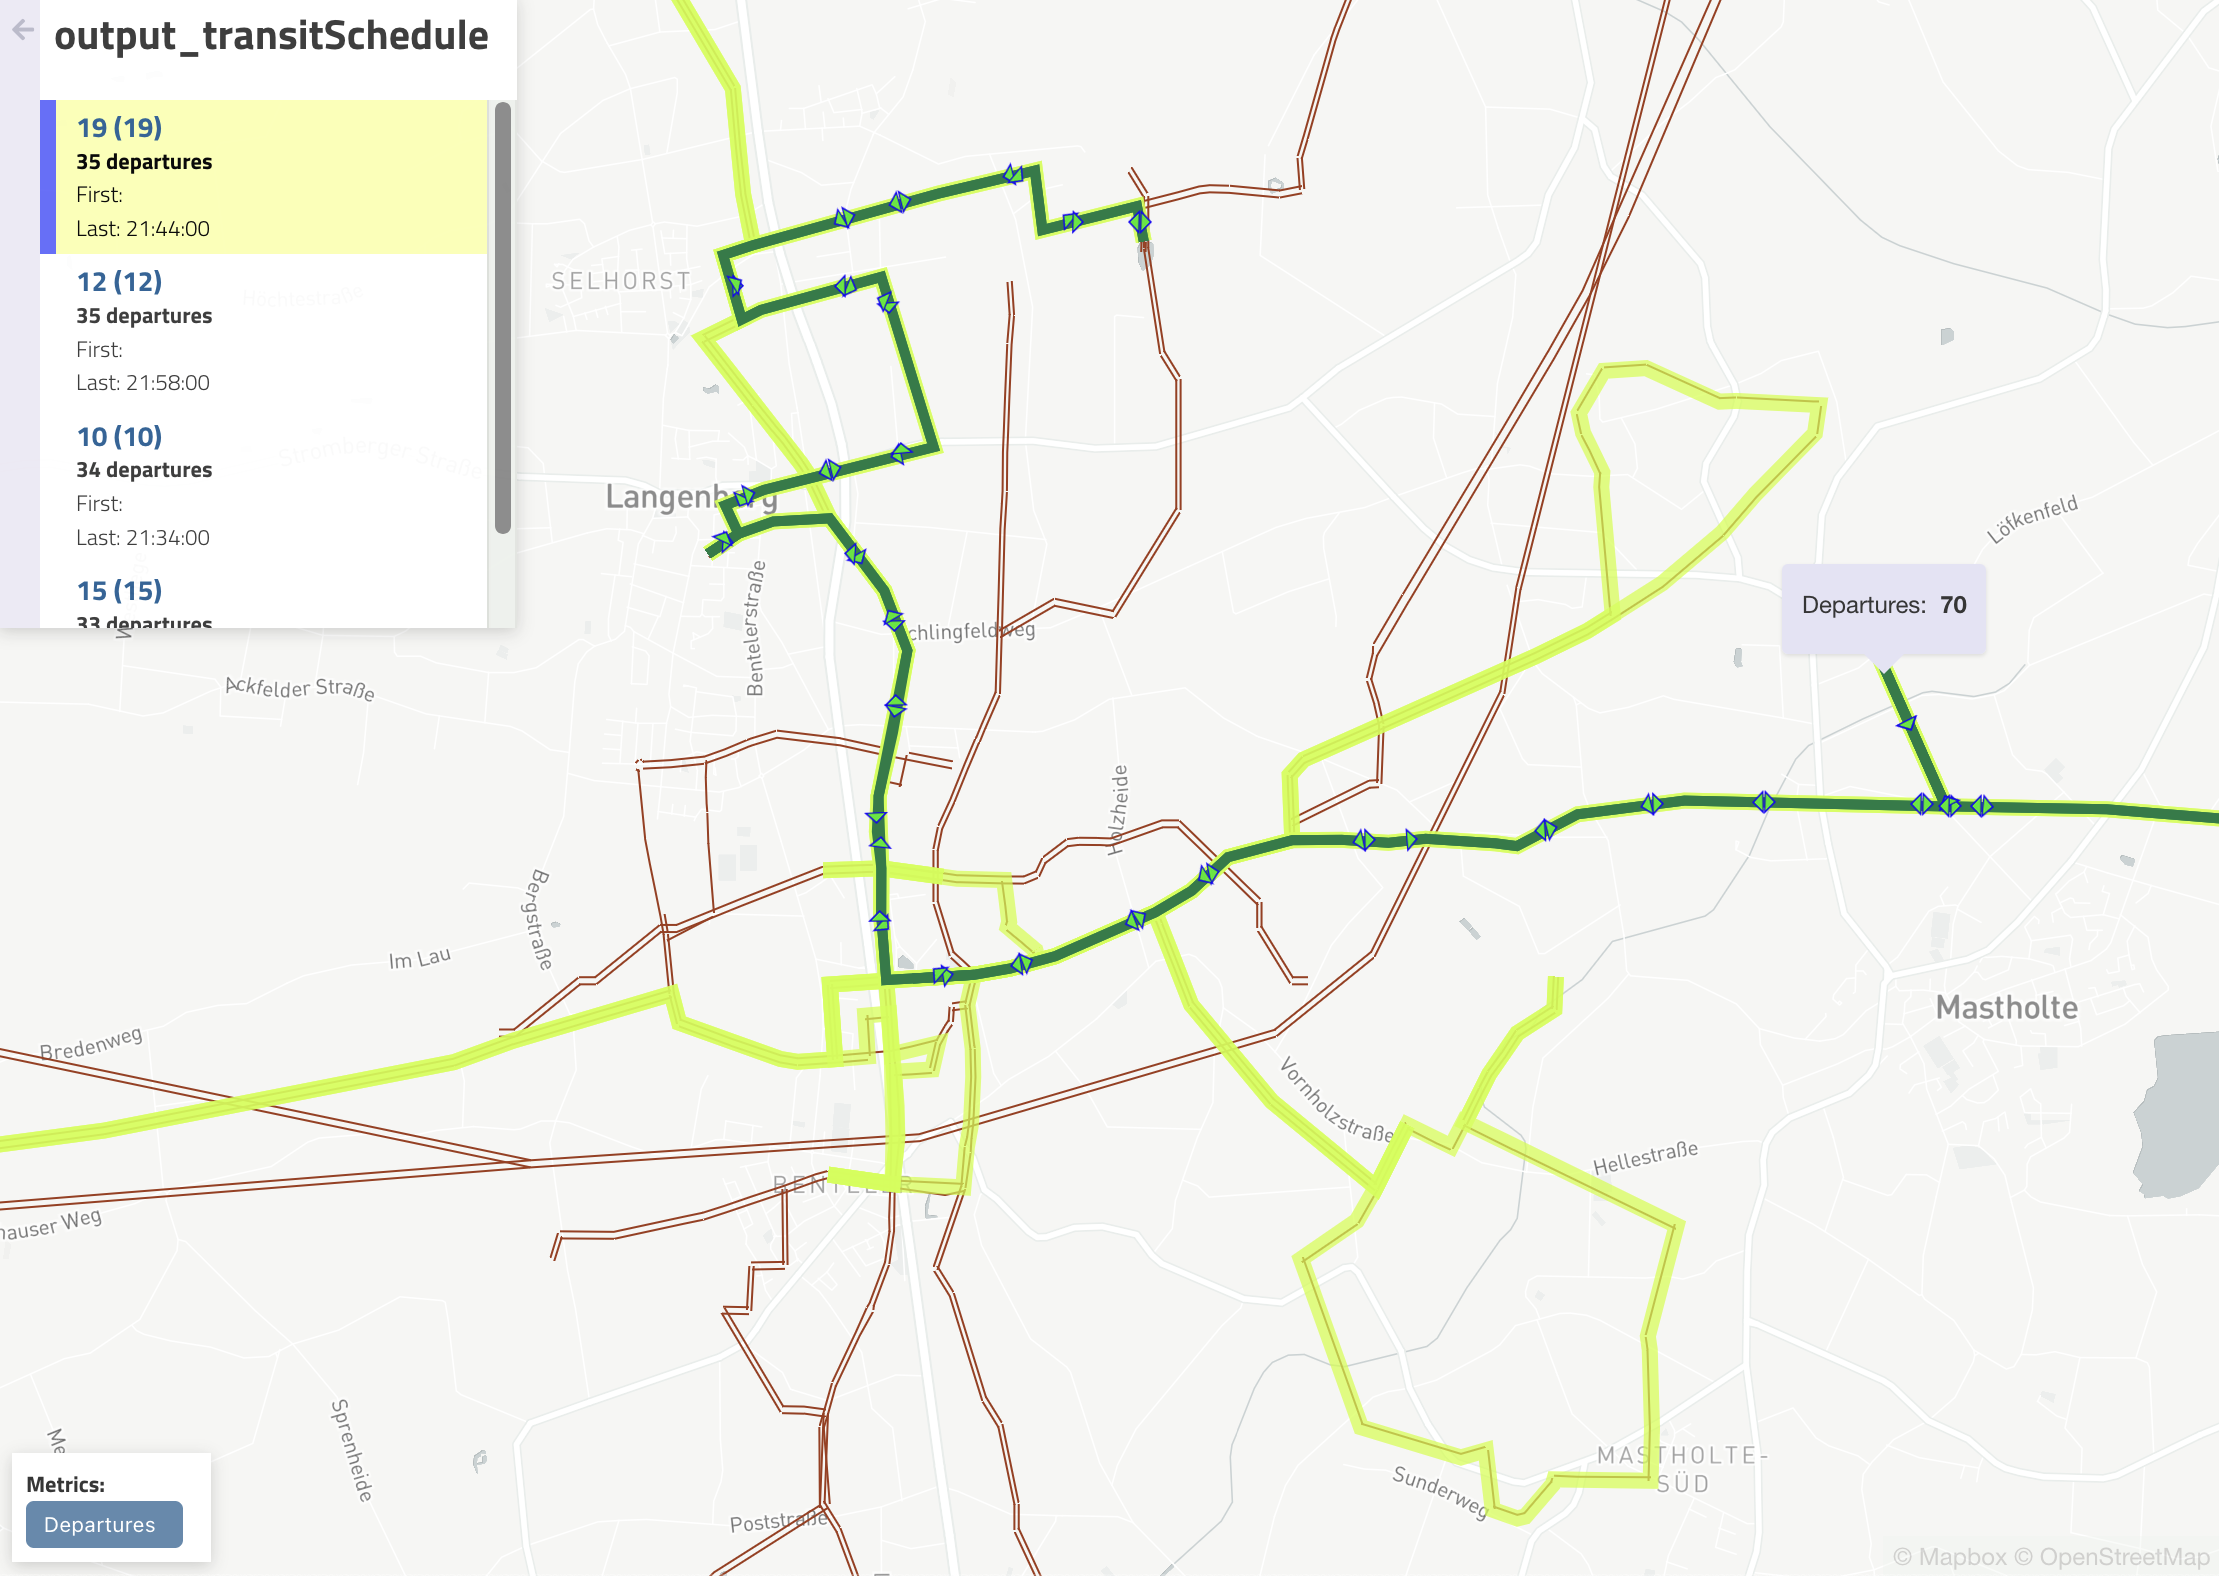
\includegraphics[width=\textwidth]{chapters/12-server-experiments/images/transit-viewer.png}
  \caption[Web-based transit network viewer]{Web-based transit network viewer. This depicts the public transit network of Cottbus, Germany, a small city in eastern Germany. One central link is selected, with the various transit routes using that line highlighted in yellow and green.}
  \label{fig:transit-viewer}
\end{figure}

As the user highlights routes in the detail view, or selects different road or rail facilities on the map, the colors and details update immediately, allowing interactive exploration of the transit schedule.

Users provided positive feedback on the tool, saying that it helped them debug network errors in complex networks, and was fast and responsive. Constructive feedback highlighted initial confusion around file management and coordinate system conversion, and this feedback helped fine-tune the tool's functionality.

%% ----- GEOSERVER -----
\hypertarget{server-experiments-geoserver}{%
\section{Accessibility calculations using GeoServer and MATSim}\label{server-experiments-geoserver}}

MATSim can be used to calculate general accessibility measures, as described in \cite{ziemke2018accessibility}. For a project in Nairobi, Kenya, MATSim is used to generate accessibility measures for several different metrics such as access to drinking water, public school locations, and commercial opportunities. For each measure there are multiple scenarios such as current conditions, system breakdowns (such as a contaminated water source) and so on. The proliferation of combinations of measures and scenarios lead to the idea of using a server back-end to store results, along with a web-based front end to review results.

\gls{GeoServer}, as described in \cite{giannecchini2013geoserver}, is an open source server for sharing geospatial data.

\begin{displayquote}
\emph{``an Open Source application for the handling and dissemination of geospatial data. GeoServer provides the basic functionalities to create interoperable Spatial Data Infrastructure according to standards edited by the Open Geospatial Consortium (OGC)... GeoServer [can] ingest, manage, and serve both vector and raster geospatial data.''}
\end{displayquote}

VSP has a departmental GeoServer installation, and the outputs of the accessibility calculations can be uploaded to it easily. Thus for this experiment, instead of a fully client-side JavaScript web application, a website front end is built that accesses the data on GeoServer using the GeoServer API.

\hypertarget{server-experiments-geoserver-2}{%
\subsection{Specifying the available accessibility measures using YAML}
\label{server-experiments-geoserver-2}}

GeoServer uses a long ``string-id'' to identify datasets. This identification or ID is constructed from the scenario details. For example, the ID for the Kibera, Kenya OpenStreetMap Live scenario, examining drinking water accessibility within 50 meters, with a specific color scale for relative differences of 0.5-3.5 units compared to the base case, has a string ID of

\emph{accessibilities:ke\_kibera\_osm\_live\_50\_drinking\_water\_walk\_0.5\_3.5}.

This is quite unreadable and is too technical for outward-facing website text, so the client website reads a YAML-based configuration file (see below) which maps the many run configurations to the appropriate GeoServer IDs. The various options are then exposed in the website user interface as drop-down selections, buttons, and so forth.

YAML itself is a simple text format which uses indentation and punctuation to define and group pairs of \emph{key:value} configuration data. For example, \autoref{fig:geoserver-yaml} shows a snippet of a YAML configuration for drinking water in Kibera, Kenya.

\begin{figure}[!ht]
  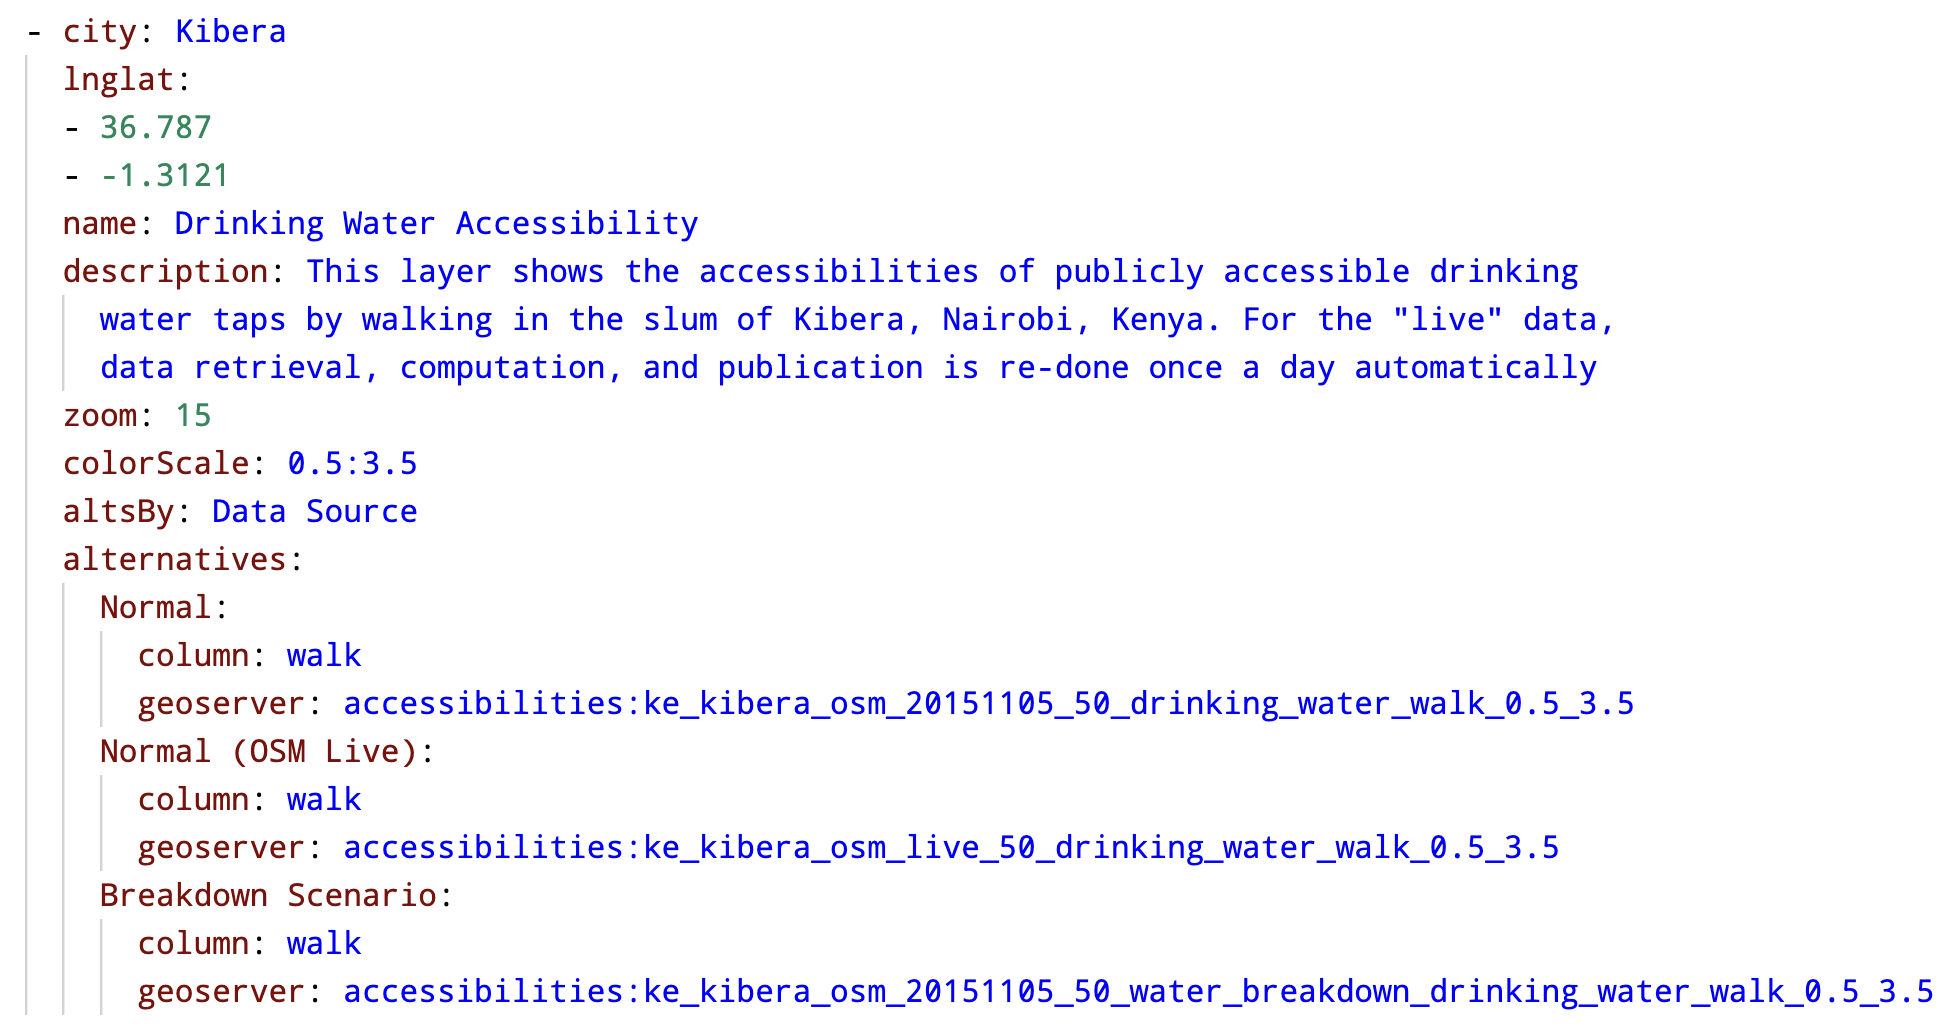
\includegraphics[width=\textwidth]{chapters/12-server-experiments/images/geoserver-yaml.png}
  \caption[GeoServer YAML configuration example]{Snippet of YAML configuration which maps user-intelligible information to GeoServer dataset IDs.}
  \label{fig:geoserver-yaml}
\end{figure}

This configuration information is read when the site is initially loaded. All of the runs defined in YAML can then be found in the user interface by selecting the metric from a dropdown and choosing the scenario for that metric with a set of buttons. The accessibility data is then pulled from the GeoServer API and displayed on top of a background map.

\hypertarget{server-experiments-geoserver-3}{%
\subsection{The Nairobi, Kenya accessibility data website}
\label{server-experiments-geoserver-3}}

\autoref{fig:nairobi} shows a typical accessibility measure displayed in the website built for the Nairobi, Kenya project. In this image, the selected metric (access to drinking water) and the scenario (normal conditions) are visible, and the grid-based accessibility values calculated by MATSim are plotted on top of the basemap. Hovering over a colored area shows the exact values for the cell in a popup hover window.

\begin{figure}[!ht]
  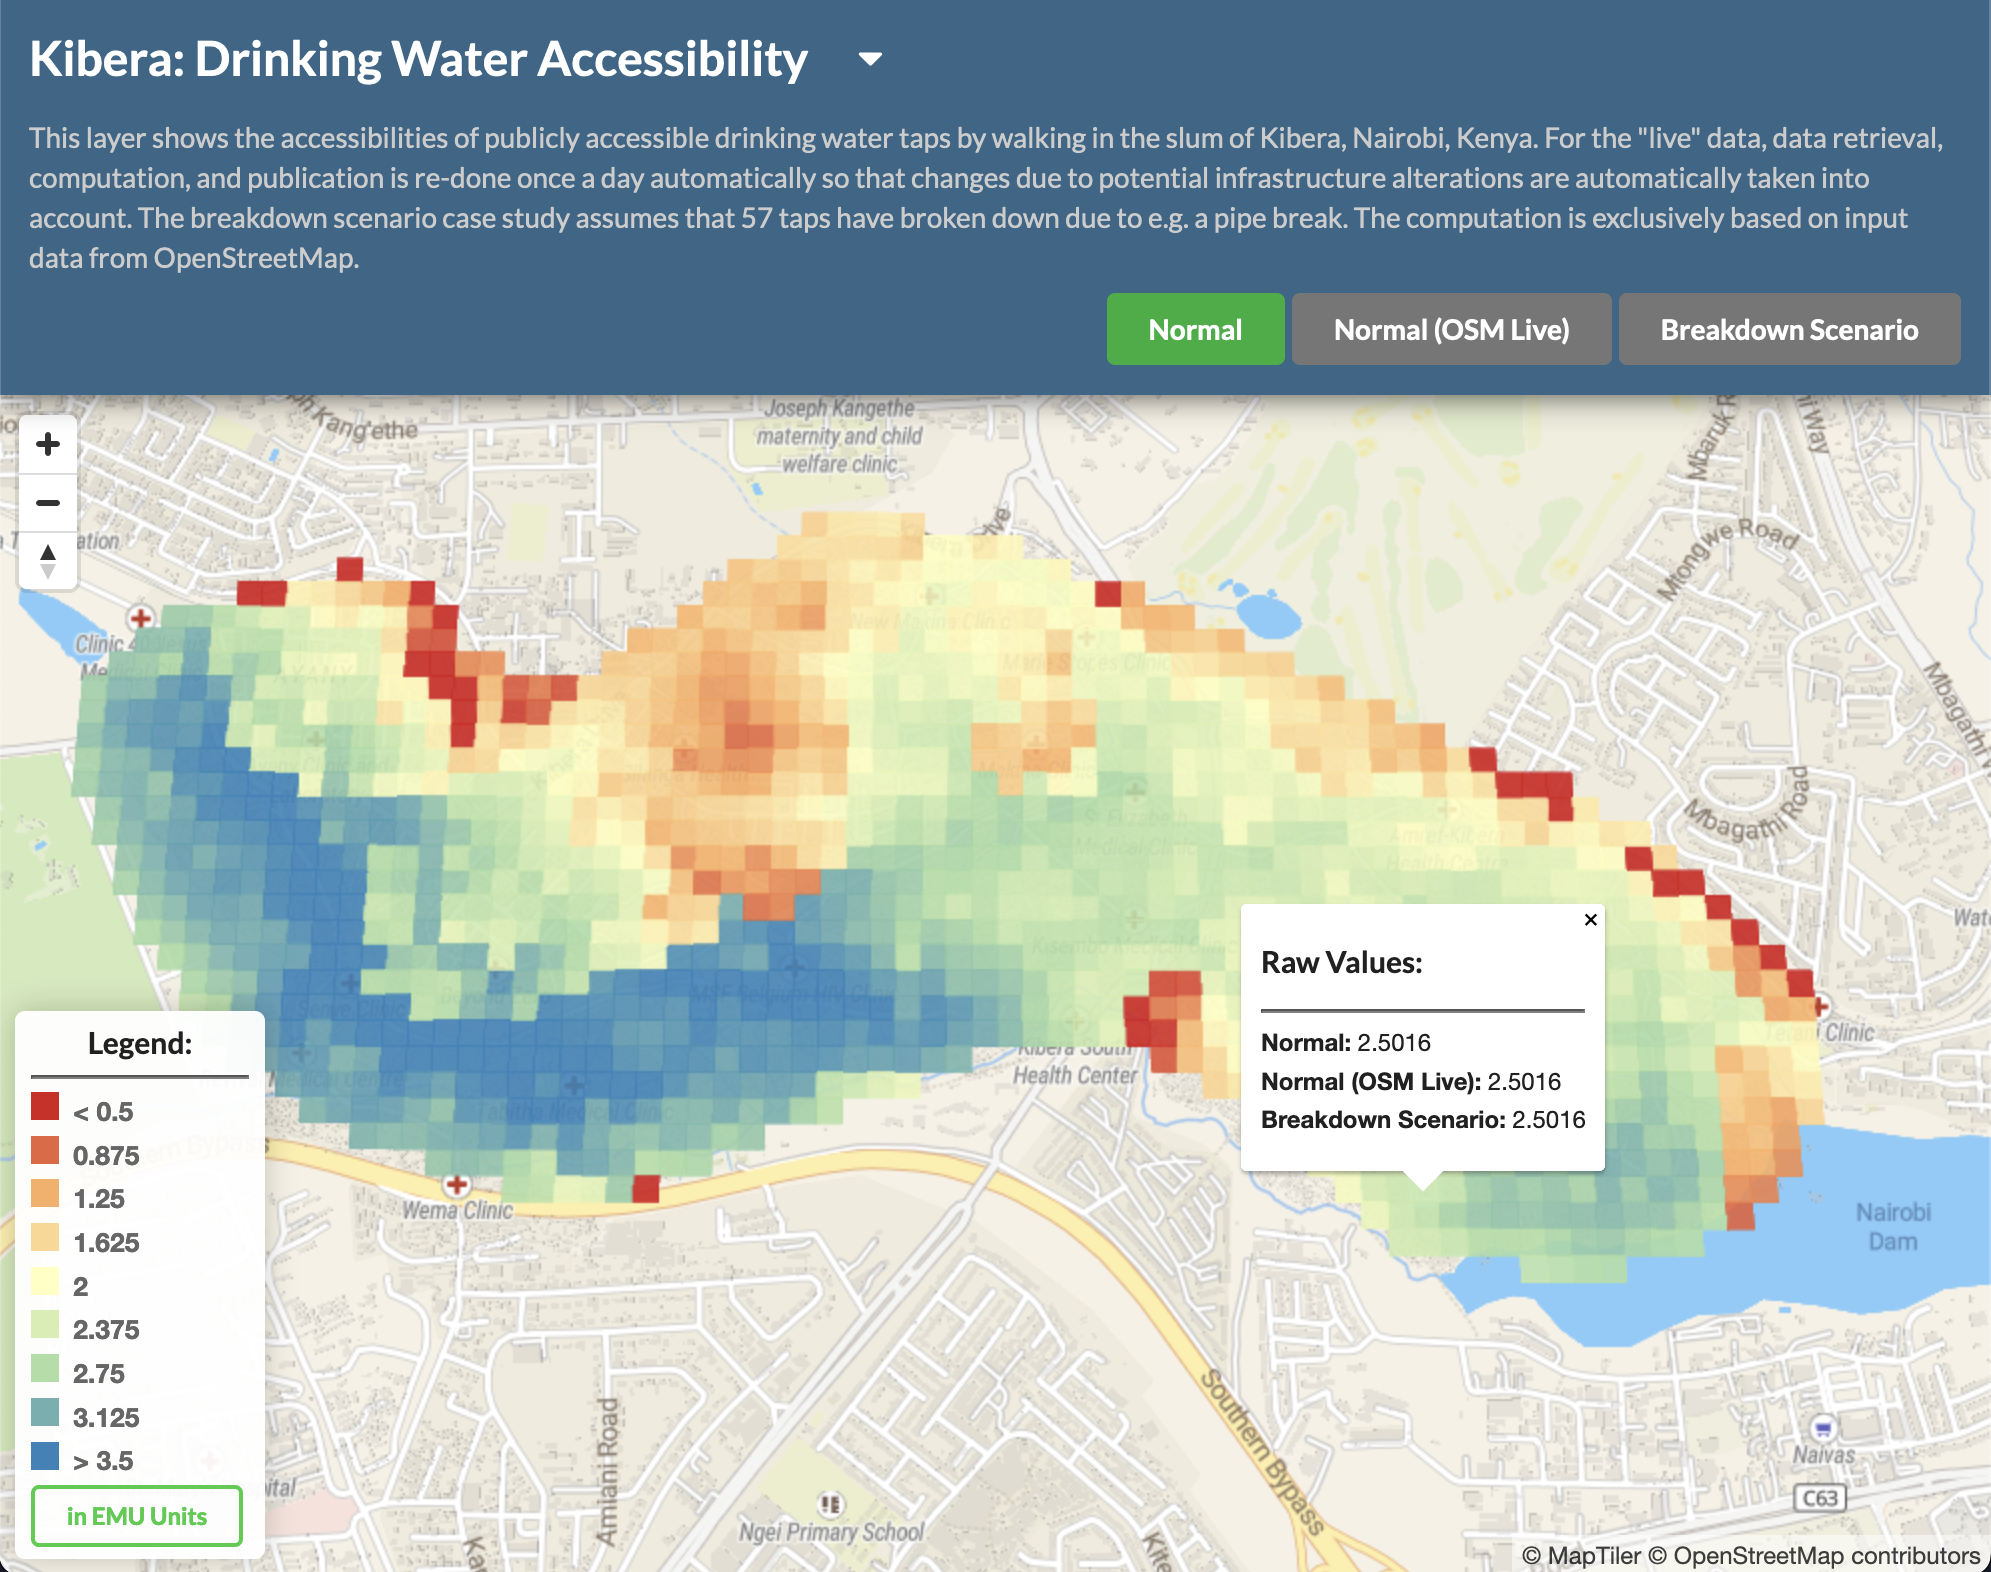
\includegraphics[width=\textwidth]{chapters/12-server-experiments/images/nairobi.png}
  \caption[Drinking water accessibility calculations, generated by MATSim]{Drinking water accessibility calculations, generated by MATSim. This interactive tool allowed users to compare accessibility calculations for drinking water, school locations, and commercial opportunities across several alternatives.}
  \label{fig:nairobi}
\end{figure}

Feedback from internal users was initially positive, as they were able to upload new runs to the server as part of their normal workflow, and updating the website only required the editing of one configuration file.

However, this approach requires manual updates from the web development team every time new data was available. For larger teams or more rapid analysis, a more streamlined and automated approach would be beneficial.

The accessibility website was not developed further after this initial experiment. Indeed, the GeoServer implementation at VSP was not used for any other purposes after this accessibility research concluded. Interviews revealed that department staff were unsure of the benefits of uploading their datasets to the GeoServer when they could instead make non-interactive maps in traditional GIS desktop software, suitable for inclusion in publishable research papers.

%% ----- EMISSIONS  -----
\hypertarget{server-experiments-emissions}{%
\section{Visualizing MATSim emission outputs}
\label{server-experiments-emissions}}

MATSim emissions outputs can be derived from simulations using standard MATSim modules, as documented in \cite{Kickhoefer2015EmissionModeling}. In brief, the levels of several emission types produced on a geographic grid-cell basis are created from the standard MATSim modules, and post-processing scripts export these values for each specific emission type.

As an experiment in how to ingest a large dataset by the web client and the MapBox GL visualization library, a new interactive website is built for displaying MATSim emissions, with the intention to load this data in its entirety. Similar to the earlier experiments, the user can either store their simulation outputs on the departmental file server or access them via a local HTTP server running on localhost.

The size of the emission output files depends on the size of the grid cells, the number of time bins, and the geographic extent of the overall area being modeled. For the Berlin experiment, one-hour time bins and 100 meter cells resulted in individual pollutant files of approximately 150 megabytes each. Being text files, they compress by around 60-75\% -- but even so, these are rather large files to try to load into a local web browser.

It does work: after loading the data, which can take about a minute on a fast, recent laptop, the map is viewable. See \autoref{fig:emissions-grid} for an example view of emissions at the grid cell level in an area near a major freeway in Berlin.

\begin{figure}[!ht]
  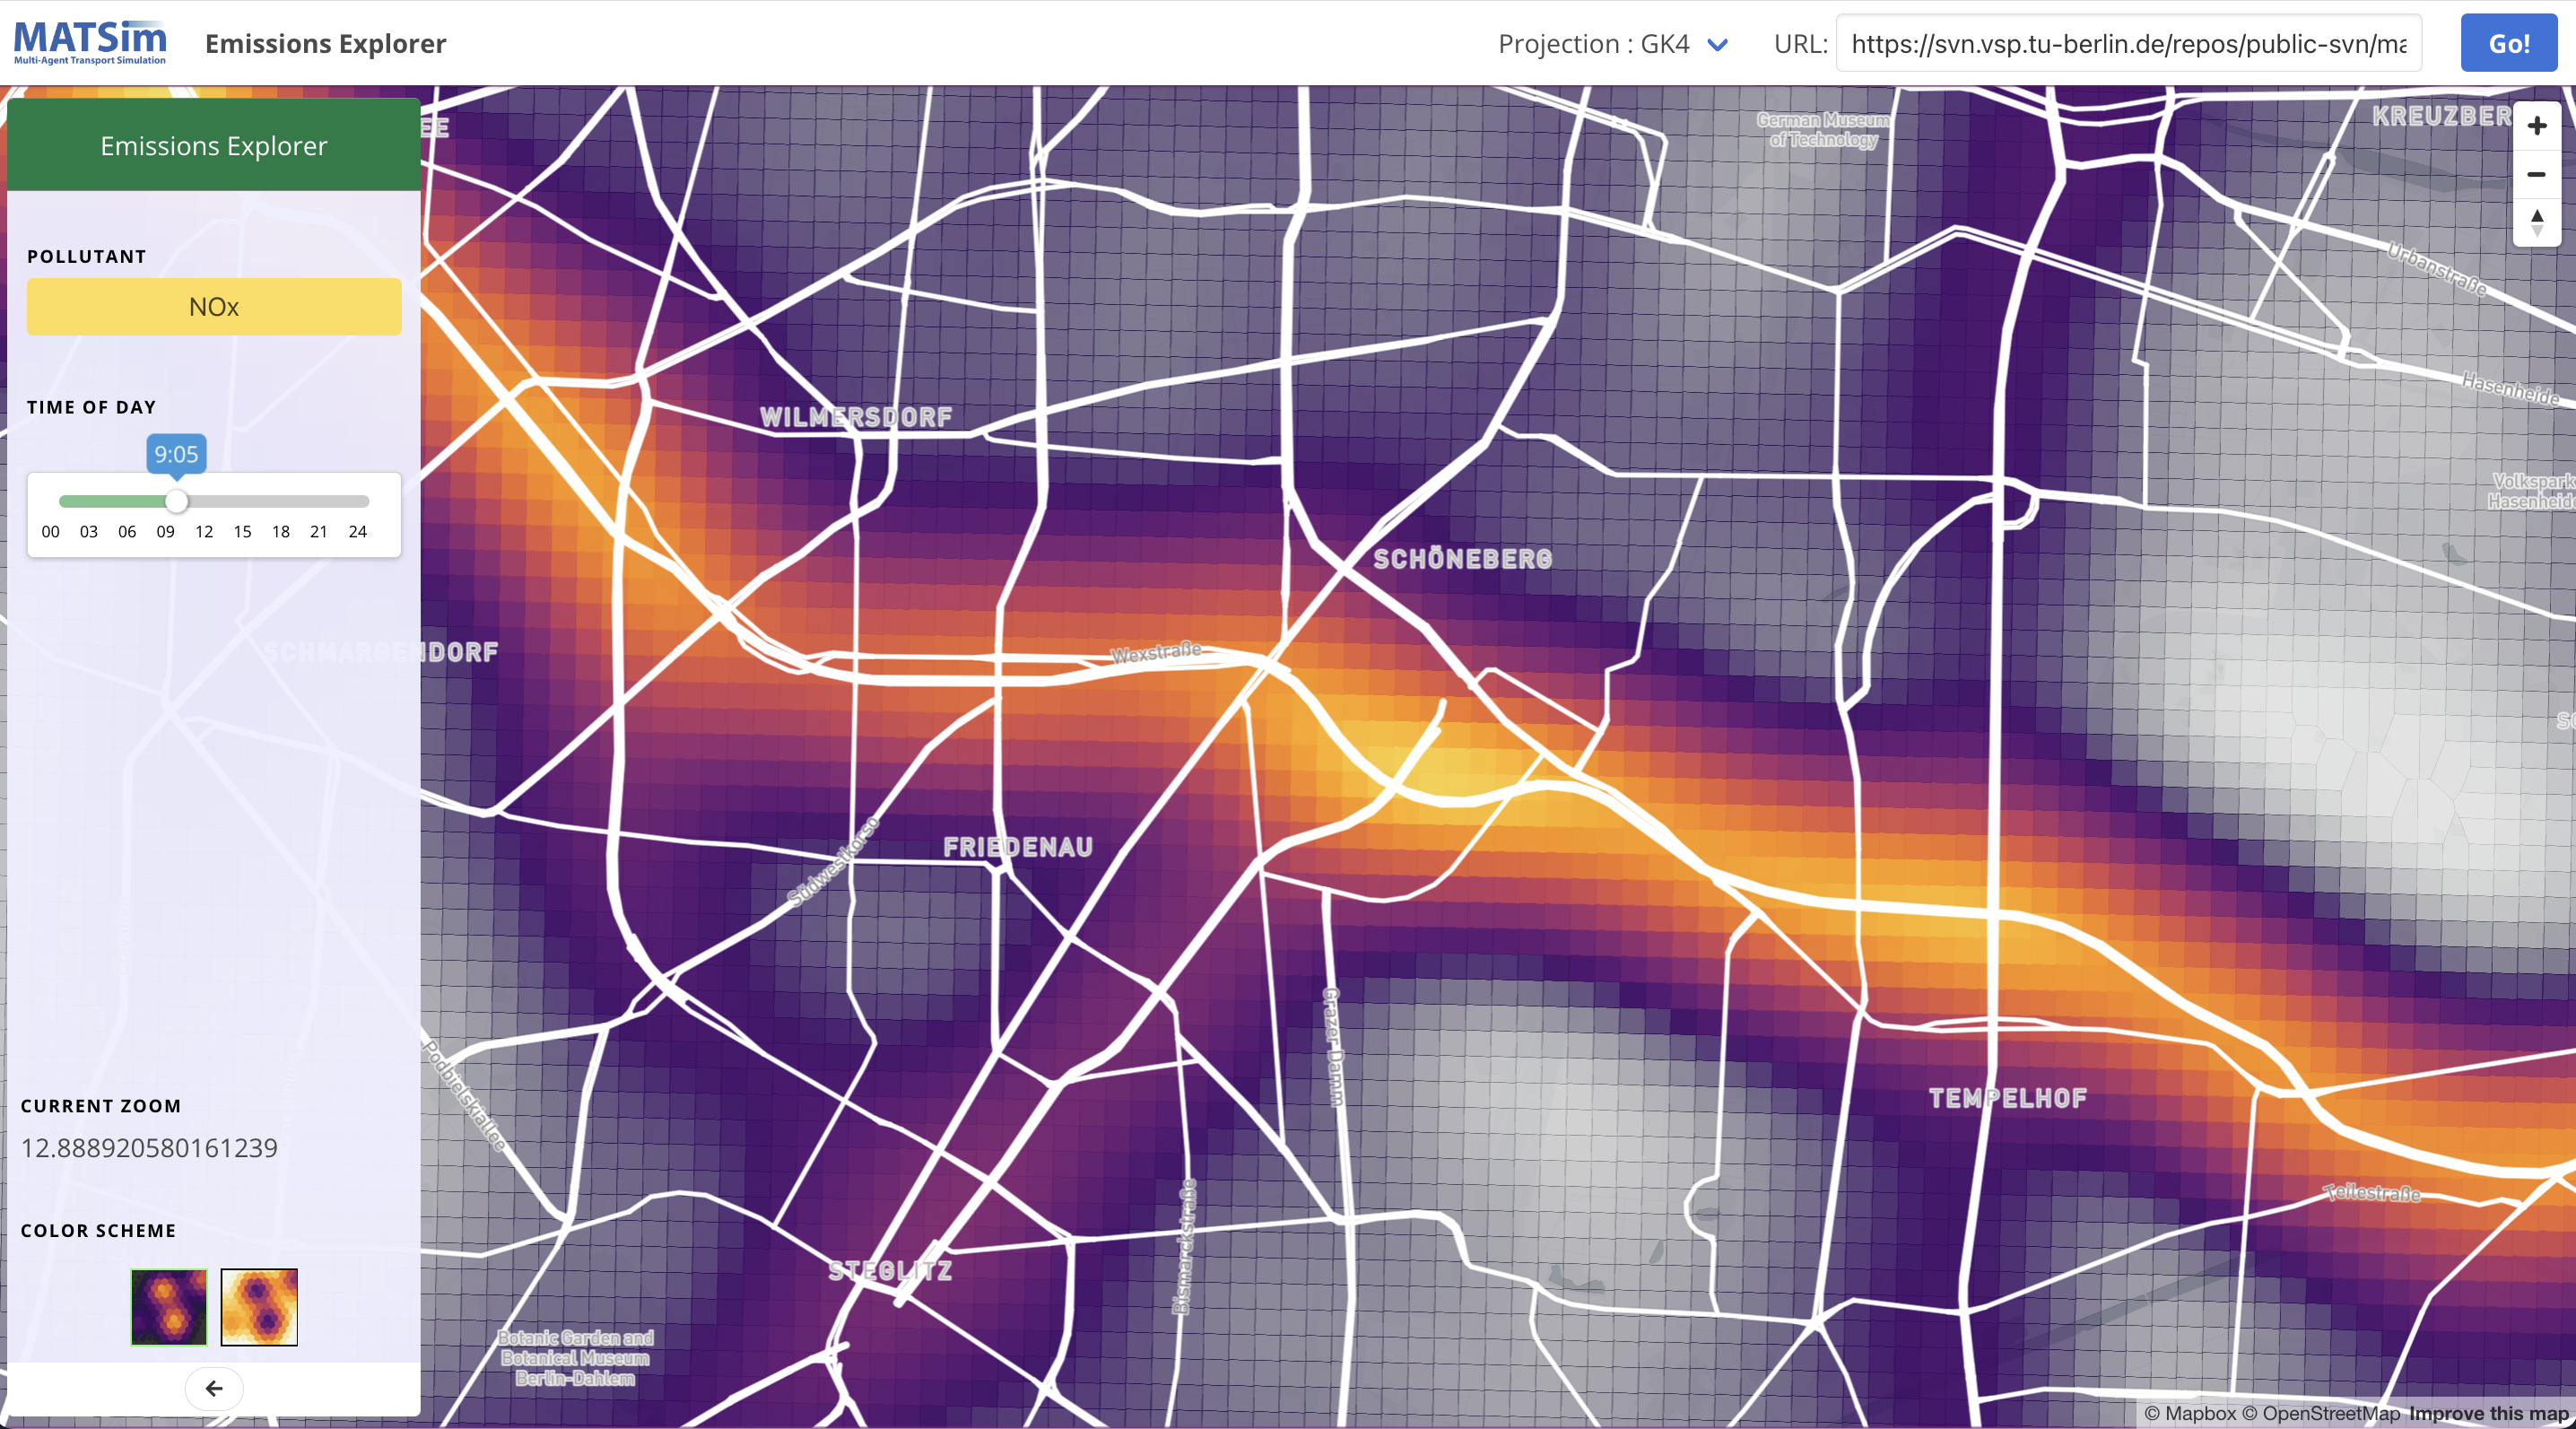
\includegraphics[width=\textwidth]{chapters/12-server-experiments/images/emissions-grid.png}
  \caption{Example grid-based emission values output by MATSim for a Berlin scenario.}
  \label{fig:emissions-grid}
\end{figure}

\hypertarget{server-experiments-emissions-lod}{%
\subsection{Level of detail}
\label{server-experiments-emissions-lod}}

A problem arises when the map is zoomed out. The MapBox GL mapping library slows down to unusable speeds when there are too many cells in the view at once. ``Too many'' depends on the speed of the laptop and power of the graphics card, but the problem occurs for even the fastest laptops available for testing.

Thus, a way to trim or reduce the amount of data being displayed is necessary. Limiting the ``level of detail'' by selecting a subset of grid cells as the map is zoomed out successfully results in the map being viewable again. As soon as the map is zoomed, this triggers a background task that filters the dataset to the visible subset of coordinates and the values thereof.

For each of these elements, a Voronai cell is calculated which surrounds the area around the selected points. Voronai is ``one of the most fundamental data structures in computational geometry'' as described decades ago in \cite{aurenhammer1991voronoi} and is well-suited to this visualization type. The Voronai diagram replaces the hard, square grid of cells with variably-sized convex polygons surrounding each selected data point, so that every point on the map is inside the cell along with the closest selected point.

This approach makes for some interesting looking plots, an example of which is shown in \autoref{fig:emissions-lod}, but it also clearly warps the values being displayed. Jagged edges around the Voronai cells are especially pronounced in areas where the emissions are dropping off rapidly, such as the areas immediately adjacent to high-emission freeway segments.

\begin{figure}[!ht]
  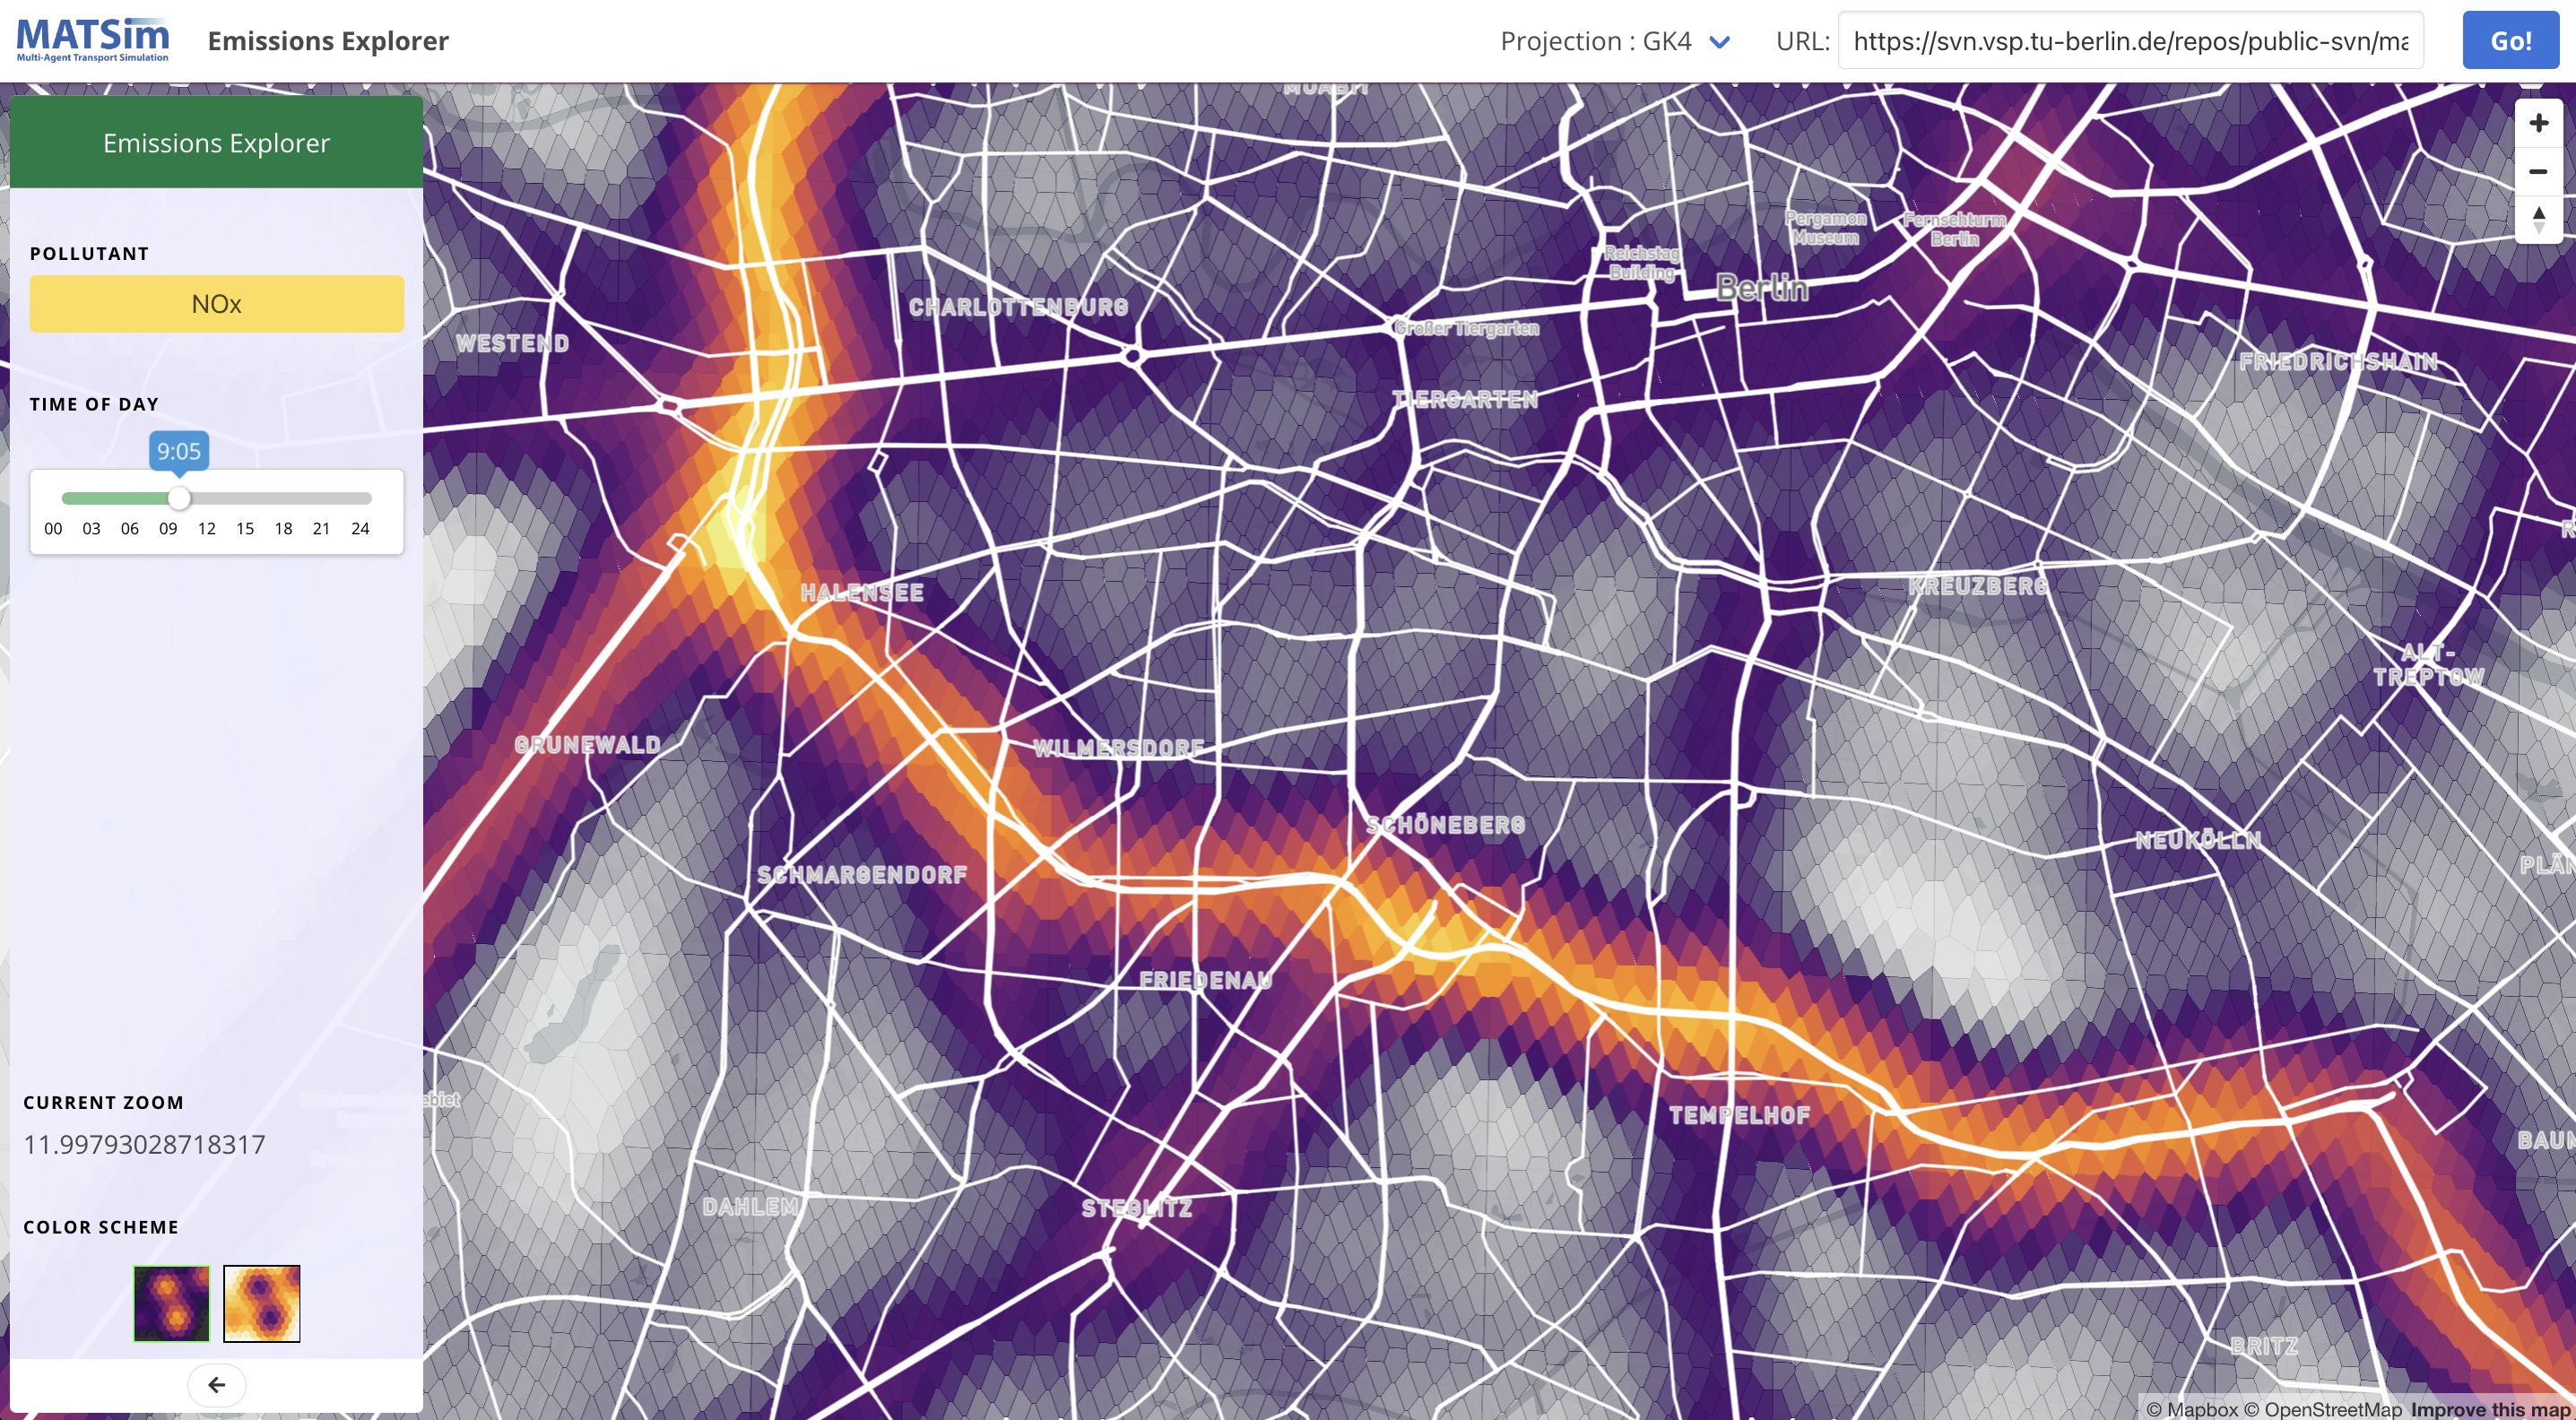
\includegraphics[width=\textwidth]{chapters/12-server-experiments/images/emissions-lod.png}
  \caption[Example Voronai areas depicting emission values for a Berlin scenario]{Example Voronai areas depicting emission values for the same Berlin scenario. This zoom level required using a level-of-detail optimization to reduce and simplify the large number of data points being drawn at the same time.}
  \label{fig:emissions-lod}
\end{figure}

The background task of calculating Voronai cells at a specified zoom level is visibly sluggish, and the results have display artifacts that may not be helpful to analysts. Between the slowness of loading the data, the sluggishness of the resulting visualization, and the compromises involved in viewing a limited level of detail at some zoom levels, this visualization experiment was not very useful for analysts at VSP.

The research on roadway emissions is published in \cite{kaddoura2022exhaust}, without reference to these visualization experiments.

%% ----- DISCUSSION AND OUTLOOK  -----
\hypertarget{server-experiments-findings}{%
\section{Discussion and Outlook}\label{server-experiments-findings}}

These initial experiments exploring use of web-based technologies to visualize MATSim simulation data result in some useful findings.

First, the management of simulation output files is complex and subject to the pre-existing habits and preferences of analysts. Feedback from analysts makes it clear that MATSim outputs are almost always very large, and moving these files around from the machine they were produced on to servers for analysis or for longer-term storage creates friction for analysts. That friction is high enough that very few researchers in the department are willing to try some of the capabilities being developed for them. The alternative, running a local HTTP server to view files on a local computer, was itself also very foreign to analysts, and created another barrier to usage. Future developments must streamline the workflow and file management.

Second, there is a limit to how much data can be reasonably ingested by a local web browser. Even on the most recent and performant laptops, some datasets are simply too large to load natively and require post-processing for aggregation, pruning, and filtering of datasets using ``level of detail'' techniques. This is a central reason why most commercially-built data analysis products rely on a back-end server which stores datasets, usually in some sort of database format, and a client front-end which displays subsets of that data as it is received. The GeoServer example above used this approach successfully. The emissions example showed the limits of the client-side approach, as the load times were unacceptable and the MapBox GL libraries could not handle the size of the datasets once loaded. (But see \autoref{ch:simwrapper} for techniques developed for successfully handling much larger datasets client-side).

Based on the results of these experiments, a client-server approach for centralizing MATSim simulation outputs and visualizations is identified as a logical next step. Creating a server-backed system has some risks as noted above, but it is the approach taken by most data-heavy websites. That system is described fully in \autoref{ch:mathub}.

%% ----- SUMMARY  -----
\hypertarget{server-experiments-summary}{%
\section{Summary}\label{server-experiments-summary}}

This chapter describes a set of web-based data visualization experiments that explore different approaches to visualizing MATSim simulation outputs in various contexts.

The public transit supply viewer allows the end user to load and explore the public transit network schedule directly from the MATSim input network and transit schedule XML files. These files are small enough to be loaded directly in the browser, and users find the tool useful in debugging the transit networks for their projects.

The accessibility data tool provides an interactive, outward-facing website that depicts accessibility datasets uploaded to a central server. The tool is feature-rich, but is limited in scope to small datasets that are uploaded manually to a specific departmental server; and ultimately does not have long-term usefulness to researchers.

The emissions data experiments test the limit of data sizes that can be ingested client-side. Files of 150 megabytes are successfully loaded, but users find the load times unacceptably slow and the operation of the website too sluggish to be useful. Smaller datasets might be more manageable, but the reality is that MATSim is used for large-scale microsimulation studies, and the size of these datasets prove too large for a fully client-side approach with the chosen JavaScript libraries and implementation.

User feedback from all of these experiments highlight the need for streamlined workflow and minimal copying of files between machines, as this creates friction for adoption.

The next chapter describes an attempt at addressing these findings in an integrated platform.


\chapter{MatHub: a client/server-based data visualization research platform for MATSim}
\label{ch:mathub}
\emph{A previous version of this chapter was published in \citet{CharltonLaudan2020WebBasedVisualization}.}

Open-source and commercial tools are available for analyzing MATSim transport simulation results, but in general these tools are installable desktop software that supports professional analyst workflows. This research builds a new open-source visualization platform for MATSim outputs that is entirely web-based. After initial experiments with many different web technologies, a client/server platform design emerges which leverages the advanced user interface capabilities of modern browsers on the front-end, and relies on back-end server processing for more CPU-intensive tasks. The initial platform is now operational and includes several aggregate-level visualizations including origin/destination flows, transit supply, and emissions levels; as well as a fully disaggregate traffic animation visualization. These visualizations are general enough to be useful for various projects. Continuing work is expected to make the visualizations more compelling and the platform more useful for practitioners.

\hypertarget{mathub-introduction}{%
\section{Introduction}\label{introduction}}

MATSim is an open-source framework for implementing large-scale agent-based transport simulations (\cite{MATSimBook}). MATSim is widely used for transportation research in academic settings, and is gaining momentum as a tool ready for practice in real-world planning contexts.

There are many tools available for analyzing MATSim results, both open-source and commercial. Typically, analysts can choose either the free tool OTFVis (\cite{Srippgen2015OTFVisInBook}) or the commercial software Via (\cite{Rieser2015SenozonViaInBook}), both of which are desktop software packages requiring installation as well as a fair amount of technical acumen to operate. Alternatives to these tools include the more general-purpose desktop mapping software packages such as QGIS\footnote{QGIS available at \url{https://qgis.org}} and ESRI ArcGIS\footnote{ESRI ArcGIS available from \url{https://www.esri.com}}, or statistical software packages, again all of which require installation and expertise to use.

As MATSim moves from the confines of academic research to a more public-facing role, a notable gap is apparent: there are scarce web-based interactive tools available for disseminating MATSim data and results. This creates a challenge for using MATSim in public policy settings: the only people who can meaningfully examine and explore results are those who have extensive technical knowledge and access to the specialized software and large datasets involved.

This research explores one way to fill this gap: building an open web-based data visualization platform which is specifically designed to complement MATSim.

\hypertarget{mathub-motivation}{%
\section{Motivation}\label{mathub-motivation}}

The rapid advancement of Internet browsing technologies in the last five years has enabled the web browser to do things much more ``application''-like than ever before: background processing, three-dimensional rendering using GPU acceleration, offline support, and more. The combination of these technologies and their standard implementations on every popular hardware type and operating system now makes the web a very compelling platform.

For MATSim, the research question is: could a web browser really be useful for exploring and delivering results when the datasets are so large? Answering this question is the primary motivation for this research. Essentially: has the web become powerful enough for MATSim?

Currently, analysis of MATSim outputs ends up in research reports, PDFs, video screen-recordings, and presentations. An online dashboard of results which a user could explore and manipulate would not only be more interactive, but might also reveal findings that the original analysts hadn't anticipated.

\hypertarget{mathub-requirements}{%
\section{Requirements}\label{requirements}}

The research team at Technische Universität Berlin had several ``blank slate'' discussions before any code was written: meaning, if we could start at the very beginning and design something completely web-based and open, what would the bare minimum requirements be for it to be truly useful? The following requirements emerged from those discussions.

\hypertarget{requirement-1-web-browser-based}{%
\subsection{Requirement 1: Web browser-based}\label{requirement-1-web-browser-based}}

Given the above-stated motivation and hypothesis that the modern web platform is ready for large-scale visualization tasks, the most obvious requirement is that the product of this research must work with any modern web browser.

Several specific web technologies developed and made widely available in recent years enable us to perform this research: HTML 5, CSS 3, WebGL, ECMA Script 6, and Web Workers. Briefly, these technologies are:

\begin{itemize}
\tightlist
\item
  \textbf{HTML 5} improves and standardizes the ``document model'' of
  what constitutes a web page and how it is specified.
\item
  \textbf{CSS 3} is a styling language that enables fine-grained layout
  and styling of individual elements on a page. CSS 3 defines in a
  consistent, standard way the details of elements including color,
  size, layout, and animation of page elements.
\item
  \textbf{WebGL} provides in-browser support for the 3D-accelerated
  graphics capabilities of modern machines.
\item
  \textbf{ECMAScript 6} is an updated (2015) version of the venerable
  JavaScript scripting language that has been part of the web platform
  since the early 1990's. Recent versions of JavaScript eliminate the
  more problematic aspects of the language and make it easier for
  developers to create bug-free, efficient code.
\item
  \textbf{Web Workers} are a recent (2013) addition to the web platform
  that allow background thread processing for long-running tasks. Before
  Web Workers, there was no way to run truly multi-threaded code inside
  a browser.
\end{itemize}

A complication in web development is that the major web browser vendors implement these technologies on their own timelines, some much more rapidly than others. Further complicating things is the reality that end users do not always upgrade their browsers frequently (or at all). This creates a landscape where there is a technology adoption curve with a very long ``tail''. Thus, developers of every web site need to make a conscious decision about where to draw the line -- choosing necessary technologies for their site to operate correctly, while knowing that some users with older browsers will either have a suboptimal experience or have no access to the site at all.

This research deliberately explores the latest \emph{standard web technologies}, with the expectation that access to these technologies will become more and more common in the future. Thus, it targets the most recent versions of modern web browsers as of 2022, including Google Chrome, Mozilla Firefox, and Apple Safari. All three browsers fully support the above-listed technologies, and importantly, all three auto-update automatically, ensuring that most users of those browsers stay current as these technologies evolve.

\hypertarget{requirement-2-open-source}{%
\subsection{Requirement 2: Open
source}\label{requirement-2-open-source}}

The entire project, including all front-end (browser) and back-end (server) code, must be fully open-source.

No proprietary or closed licensing schemes were considered, primarily because excellent proprietary visualization packages for MATSim already exist. Creating a competing product would be duplicative and unnecessary, and would not further the research goal of determining whether web-based technology is now advanced enough to work with MATSim outputs. The goal of this research is not to replace existing, proprietary solutions, but rather to complement them.

The software developed as part of this research is licensed entirely with the GNU General Public License v3, commonly known as the ``GPL''\footnote{GNU General Public License (June 29, 2007). Version 3. Free Software Foundation. Available at \url{https://www.gnu.org/licenses/gpl.html}}

This matches the license of MATSim itself. Several other open-source licenses were considered, including the MIT License and the Apache Public License, but the benefit of sharing a common license with MATSim outweighs any perceived benefits of switching to other open licenses.

\hypertarget{requirement-3-use-good-defaults-with-minimal-configuration-and-be-opinionated}{%
\subsection{Requirement 3: Use good defaults, with minimal configuration, and be opinionated}\label{requirement-3-use-good-defaults-with-minimal-configuration-and-be-opinionated}}

Since its inception, the web platform has had a relentless focus on simplicity and smooth user onboarding. Users are accustomed to being immediately familiar with a site -- often within seconds of their first interaction. Because of this expectation, it is critical that this research follow current best practices for user interface (UI) and user experience (UX). Specifically, that means using familiar UI paradigms such as navigation bars and breadcrumbs, separating configuration from usage, limiting settings and options to the bare minimum, and being ``opinionated'', i.e.~encouraging a correct way to accomplish a task.

This approach is dissimilar to some data exploration tools (e.g., QGis and Via) where extreme configurability is emphasized. Rather than providing myriad options for details such as scales and color ramps, our research focuses on choosing good defaults and determining whether that is sufficient for the software to be useful.

\hypertarget{requirement-4-an-extensible-platform}{%
\subsection{Requirement 4: An extensible platform}\label{requirement-4-an-extensible-platform}}

Every data visualization use case is different; there is no way to anticipate how the tool will be used. If the platform is too generic, it will be not at all useful. Conversely, if only hard-coded visualizations are created for specific projects, it will be relegated to ``demo-ware'', meaning it is a successful technology demonstration but not actually useful for real users.

To fulfill this requirement the software platform will need to be extensible: basic capabilities and templates will be provided, but a user with some level of coding skill should be able to create new visualizations that are not anticipated by the researchers.

\hypertarget{mathub-initial-experiments}{%
\section{Initial experiments}\label{initial-experiments}}

It is no exaggeration to state that the JavaScript code library ecosystem is extremely, enormously large. Thousands of libraries and packages are available on a common centralized JavaScript repository known as ``NPM'', and there are often multiple packages that do similar things. As a developer, one must assess and select from these packages or choose to solve a problem by writing code by hand. Of course these libraries are of varying levels of popularity and quality.

Based on the requirements laid out above, some initial experiments were carried out to assess various approaches before committing to a technology stack.

\hypertarget{mathub-visualizing-time-dependent-data-on-a-geographic-map}{%
\subsection{Visualizing time-dependent data on a geographic
map}\label{visualizing-time-dependent-data-on-a-geographic-map}}

Two popular web-based JavaScript libraries were tested for displaying geographic data; Leaflet and Mapbox GL. A simple test case comprised of MATSim simulation outputs was developed, with the goal of displaying aggregated roadway link volumes by time of day.

Leaflet (leafletjs.com) is very popular and its application programming interface (API) is a bit simpler than that of Mapbox GL. Leaflet uses background map ``tiles'' at specific zoom levels, and layers data on top of those base maps. With small networks (we tested Cottbus, Germany, a small city of 100,000 inhabitants) Leaflet performed well, but medium-sized and large-sized networks with many elements visible at once suffered from noticeable performance degradation. This was problematic, as this was the simplest use-case envisioned.

Mapbox GL (mapbox.com) fared much better, apparently better-suited to displaying large datasets with many visible features simultaneously. In addition, Mapbox GL's use of 3D vector graphic mapping instead of preset tiles made for a much more pleasing user experience, with smooth animations between zoom levels and better background processing during page loads. For these reasons, Mapbox GL was chosen as the base map for the remaining geographic visualizations.

\hypertarget{visualizing-non-geographic-data}{%
\subsection{Visualizing non-geographic data}\label{visualizing-non-geographic-data}}

There are hundreds of data visualization libraries available for the web which provide ways to produce charts and plots of varying complexity. Our requirement of using open-source code narrows the field considerably.

After experimenting with several packages including D3, Raphael, Morris and others, the package Vega-Lite (\cite{Satyanarayan2016vega}) exhibited many of the characteristics desired. Notably, Vega-lite follows a ``grammar of graphics'' declarative syntax, as popularized by Wilkinson (\cite{Wilkinson2012grammar}), and this grammar allows concise description of the meaningful components of a graphic. An added benefit is that graphs and charts can be downloaded in image format or in Vega source format, which is helpful for other researchers wanting to learn how to use the data format themselves.

\hypertarget{dealing-with-large-datasets}{%
\subsection{Dealing with large datasets}\label{dealing-with-large-datasets}}

MATSim network files are small enough to fit in RAM, but MATSim plan files and event files can be much larger than RAM, necessitating careful consideration about how to handle them.

Modern browsers allow access via API to a data storage area that is unique per hostname, e.g. http://mysite.com is allowed some storage on the local machine. Initial experiments revealed that each browser vendor implements this storage differently, with very strict limits on the absolute amount storage available, sometimes based on how much free space remains on the user's machine. It became apparent that this local browser-based storage would not be sufficient for MATSim outputs. Running a local file-server process would allow browser access to a specific folder on the machine, which might be nice for advanced analysts but violates the research goal of being fully web-based on the client end. Thus, a client-server paradigm emerges as the only truly viable alternative, and indeed this is how most websites operate today: the browser is the front-end to the heavier processing and storage tasks that happen on someone else's server. Note that ``someone else's server'' is usually referred to as ``the cloud''.

\hypertarget{mathub-platform-architecture}{%
\section{Platform architecture}\label{platform-architecture}}

A client/server architecture was chosen for this research based on the initial experiments described above.

The research team authored back-end server software for file storage, user authentication, and data pre-processing. Due to space considerations, this paper does not delve into the details of those components. Suffice it to mention that the front-end communicates with them to establish what resources a user has access to, and provides an application programming interface, or API, with which to query and fetch available files and resources. The code for those servers is also open source, and may be the subject of future papers.

The front-end architecture has several interacting components:

% ------------------------------------------------------
\hypertarget{mathub-build-system}{%
\subsection{Build system}\label{build-system}}

The build system of a modern web application is fairly complex and the JavaScript ecosystem changes rapidly. After numerous iterations, the current build system comprises a series of individual tools that all work together to produce the final assets that get sent to a user's browser. Those tools include the Vue command line interface (CLI), the NPM package manager, webpack, babel, and TypeScript.

Notably, the initial codebase was migrated to the TypeScript language midway through development, as the benefits of a strongly-typed language were perceived to be worth the development time. TypeScript is a separate language from JavaScript, and enforces type annotations for variables and adds additional features such as enumerations. The TypeScript compiler then converts TypeScript code into ECMAScript 6 JavaScript, which can be run in the browser (as browsers do not support TypeScript natively).

% ------------------------------------------------------
\hypertarget{vue-single-page-application}{%
\subsection{Vue Single Page Application}\label{vue-single-page-application}}

The primary framework used to build the application is known as ``Vue JS''\footnote{Vue framework, available at \url{https://vuejs.org}}. Vue is a framework for building interactive user interfaces on the web; essentially it provides the glue between the items a user clicks and the code that runs when they do so. Vue provides many services which allow a web page to behave more like a full-featured application, including state management, routing between different URLs, and componentization of code in a way that encourages code reuse and loose coupling. Vue depends on JavaScript, which means it does not work on for users who have disabled scripting in their browser.

Vue is most often used to write so-called ``single page applications'' which are websites that behave like desktop applications. Most large, popular websites such as Github, Twitter, and Facebook all employ this paradigm, meaning the site handles page transitions and URLs as if they are all in one common namespace, and the user thinks less about visiting URLs and more about navigation through visual components to accomplish tasks. This matches our use case precisely.

Vue components each encapsulate the three elements required for the modern web: HTML layout, JavaScript code, and CSS formatting. Components only interact with each other through well-defined pathways of properties and events, which greatly improves debuggability.

Note that Vue is just one of literally scores of web frameworks which all do essentially the same thing, providing interactivity to websites via JavaScript. Other frameworks such as React, Angular, and Svelte were considered but Vue was chosen due to its excellent documentation and support, and its nice "middle ground" between being lightweight and featureful.

% ------------------------------------------------------
\hypertarget{mathub-visualization-plug-ins}{%
\subsection{Visualization plug-ins}\label{visualization-plug-ins}}

One of the main requirements of this research is to produce a system where new visualizations can be produced rapidly and added into the existing framework to generate new capabilities.

The Vue component architecture enables this. To create a new visualization, a developer copies an existing ``blank'' visualization template and gives it a new name, specifies the file inputs and parameters required, and then uses the above-described libraries to modify the code per their needs.

This currently requires ample coding skill in JavaScript; it is not a system that is point-and-click like an online data exploration tool. Experience with other similarly-designed platforms suggests that software-minded analysts or modelers would be able to extend the platform, but typical end users would not. Most transport analysts are not JavaScript web programmers nor do they want to be. MatHub might be sufficient to meet the needs of users without them having to resort to coding extensions themselves.

% ------------------------------------------------------
\hypertarget{mathub-results-the-current-state-of-the-tool}{%
\section{Results: the current state of the tool}\label{results-the-current-state-of-the-tool}}

A working instance of the platform went live on the Internet in 2019.\footnote{Site was live at \url{https://viz.vsp.tu-berlin.de, now defunct as of 2022}} Sample datasets were uploaded, and pre-built visualizations were publicly accessible, as a demonstration of the platform's current state. A user login system was developed so that internal researchers could extend and experiment with the system, without exposing data or work-in-progress to the public.

Basic user, project, and file management capabilities were operational. This included grouping files by model run or by other user-defined tags.

Several types of aggregate visualizations were developed:

\begin{itemize}
\tightlist
\item
  Origin/destination flows between aggregate areas, so called ``spider
  diagrams''
\item
  Link flows, by time of day and mode
\item
  Transit supply explorer, which displays all transit routes and allows
  the user to see which routes serve specific stops and links.
\item
  Sankey diagrams, which can be used to depict changes/flows between
  between scenarios across multiple choices, such as shifts in mode
  between two scenarios (see Figure 1d)
\item
  Emissions levels on a geographic hexagonal grid basis
\end{itemize}

In addition, one disaggregate animation was available:

\begin{itemize}
\tightlist
\item
  A vehicle flow simulation, showing individual vehicle agents in
  real-time on the network.
\end{itemize}

See the set of screenshots in figure \ref{fig:mathub-examples} for examples of the final state of the user interface. Note of course that the tool demos better live than in screenshots, as the whole point of this research is to develop an interactive tool.

\begin{figure}
  \centering
	\begin{minipage}{1.0\textwidth}
  \includegraphics[width=\textwidth]{chapters/13-mathub/images/all-figures.png.pdf}
  \caption{MatHub sample visualizations, a - f. File management dashboard and examples of vehicle animations, transit and roadway volumes, and aggregate summary statistics are shown.}
  \label{fig:mathub-examples}
	\end{minipage}
\end{figure}

% ------------------------------------------------------
\hypertarget{mathub-workflow-feedback}{%
\subsection{Workflow feedback}\label{workflow-feedback}}

Initial prototypes of the tool did not meet the needs of test users. Problems included: difficult discerning which files were which; inability to efficiently use the model run tagging feature (in which a user could mark sets of files as belonging to a particular MATSim run); separate user logins causing data to be inaccesible to team members working on the same projects (resulting in everyone using a common ``team'' login, against best practices); private projects ``leaking'' onto the public website; and myriad usability bugs in the data visualizations themselves.

These usability problems were eventually solved by surveying other technical websites which organize and present large amounts of data. One website in particular, Github.com, was found to be well-liked by test users and has a similar hierarchical view of data: users can belong to organizations, and both organizations and users can create projects (``repositories'' on GitHub) which may large numbers of files.

By adopting a file, project, and user paradigm similar to that employed by GitHub, users were immediately more familiar and had less to learn. The site now adheres to this so closely that test users refer to the platform as ``MatHub''.

Longer term, however, further problems were noted. Most importantly, team members felt that the capabilities did not offer them visualizations beyond what they could create in other software packages. The promise of online dissemination of results was not compelling enough to justify the uploading of datasets to a separate visualization system. At least internally, analysts were most interested in publishing papers and producing high-quality image files for submission to journals. Without external-facing clients, the online functionality was merely nice to have, but not actually urgently necessary. As time went on into 2019 and 2020, the site was used less and less.

Internally this triggered some serious discussions about the viability, usefulness, and need of the platform. Given that this was just the first usable version, it seemed prudent to continue some further iteration on the platform to try and make it more usable and useful to internal users.

% ------------------------------------------------------
\hypertarget{mathub-performance}{%
\subsection{Performance}\label{performance}}

Even with modern hardware and the latest browsers, it is quite challenging to produce performant, visually pleasing results with disaggregate MATSim data. The vehicle flow simulation depends heavily on the back-end server to produce and deliver simulation ``frames'' to the browser in real-time, so that the browser simply has to render the data.

Various levels of aggregation make MATsim data much easier to visualize, as is reflected in the number of different visualizations this research was able to produce with aggregate data in a short time frame.

\textbf{Preprocessing.} The traffic animation and the emissions ``hex grid'' visualizations both rely on back-end server processes to preprocess the raw MATSim event outputs. This takes anywhere from a few seconds to many minutes, depending on the size of the simulation that is run. The preprocessing only needs to occur once, and thereafter the results are cached and stored on the server. The UI presents a helpful ``still processing'' message during this stage. Unfortunately, changing some settings such as the size of the hex-grids for the emission tool means the calculations must be redone. Further work is being done to make these processes run as quickly as possible.

\textbf{Map layer limitations.} The Mapbox GL mapping library allows lines, points, and polygons to be displayed on top of (or interleaved with) a base map. There seems to be a number of map elements beyond which performance becomes very slow; various techniques can be used such as aggregating elements at further-out zoom levels to get around this. Another option is to only use Mapbox GL for the base map, and to use the WebGL graphics libraries to draw large numbers of elements directly on top of the map. This is the technique used for the traffic animation, which can easily support tens of thousands of elements (all in motion) simultaneously. For additional visualizations which have large numbers of grahical elements, more research will need to be done to layer WebGL elements on top of a base map.

% ------------------------------------------------------
\hypertarget{mathub-mobile-device-support}{%
\subsection{Mobile device support}\label{mobile-device-support}}

Initially, the research targeted desktop browsers only. The reasoning was that analysts currently use desktop software, and it would be sufficient to complement those desktop tools with a new web-based option.

However, as the tool started becoming usable by internal users, it became apparent that everyone wanted some version of the visualizations to work on mobile devices, too. It was suggested that even a read-only visualization ``viewer'' for mobile would be better than not having the tool work at all on mobile.

To address this, the layout of the main user interface needed to be redesigned, but the overall stack of web-based libraries and components chosen was already well-suited to mobile use. This effort is currently underway.

% ------------------------------------------------------
\hypertarget{mathub-conclusions-and-outlook}{%
\section{Conclusions and outlook}\label{conclusions-and-outlook}}

Experimenting with the various technologies and getting all of the disparate pieces working together was an enormous task, one which took much longer than anticipated. However, those decisions are now behind us and the platform has become stable.

A new visualization can now be generated by internal researchers in a matter of days or weeks. The researchers are admittedly very familiar with the inner workings of the system, but even so it has been encouraging to see new visualizations go from ideation to rough draft in short order.

However, none of the above-listed visualizations are particularly groundbreaking or visually stunning. And all of them could be easily created in other tools (although usually without the interactivity that the web enables). This is a bit disappointing but the open nature of the platform, requiring no software installation by end users, still has an advantage: it opens up the display of MATSim results to the public and to decisionmakers, even if they do not have access to desktop mapping or travel forecasting software.

Another use case that has emerged from these visualization experiments is a more regimented data management tool for MATSim. Currently there is no straightforward way to share MATSim datasets online. The combination of the new file storage and management capabilities along with the GitHub-like user interface provides a natural place for users to store and disseminate results.

Finally, the world has not stood still while this platform was under development. Just in the past two years, major data visualization efforts from well-funded companies such as Uber and others have been released. There are legitimate questions about how much of this work could be superseded by large, well-funded, professional coding teams.

Despite these concerns, the MATSim visualization framework is operational and is now just beginning to be useful for researchers at the department of its creation. This bodes well for further development in the near future.

All code is available on the MATSim Github site.\footnote{MATSim visualization code is available at \url{https://github.com/matsim-org/viz}}


% =============================================================================
% PART II: DATA VISUALIZATION FOR PROJECT WEBSITES:
%          Developing project portals for three large-scale simulation projects
% =============================================================================

\part{Part 2: Project Sites Using Client-Side Data Visualization Techniques}
\label{part:2projectsites}

\chapter{EpiSim and the COVID-Sim.info website}
\label{ch:covid-sim}
\hypertarget{introduction-covid-19-and-episim}{%
\section{Introduction: COVID-19 and
EpiSim}\label{introduction-covid-19-and-episim}}

In February 2020, the team at VSP began work on an extension to MATSim which soon became known as ``EpiSim.''

YY reference which paper/papers?

The EpiSim model was a novel hybrid of the agent-based microsimulation model MATSim and epidemiological infection progression models. New versions of the combined model were being released, tested, and run multiple times per week in the frenetic early days of the COVID-19 pandemic in Europe. This produced massive amounts of data from literally hundreds of model simulations -- often daily.

It quickly became apparent that the team needed a way to compare all of these runs in a visual manner, and also to be able to convey salient results to decisionmakers and the public. A web-based solution was an obvious choice for both use cases, but the many problems we encountered in modifying or enhancing MatHub made us unsure that a heavyweight client/server solution would be able to keep up with the team's needs.

We decided to take an unusual approach for such a large undertaking, which leveraged the investments already made in web-based visualization technologies but jettisoned all of the back-end servers: we rapidly built what is called a ``Single Page Application'' (SPA) that was a completely self-contained website, with no back-end server processing at all. All of the website code and all of the data files would be served ``statically'' from a simple web server.

Eventually the size of the site expanded and the data storage for model results was moved to a dedicated file server, but otherwise the overall architecture remained constant and the site continues in operation today.

This approach proved successful in meeting our team's needs, and is described fully in this chapter.

The COVID-Sim website is available at \url{https://covid-sim.info}

\hypertarget{how-websites-are-built-clients-and-servers}{%
\subsection{How websites are built: clients and servers}\label{how-websites-are-built-clients-and-servers}}

As described earlier in YY, web sites always consist of the content which is loaded into a browser, known as the ``client'', and the back-end servers which the client connects to. In the simplest case, a user points to a URL, and the browser loads the HTML index file at that location along with any other static files referenced in the HTML. This is known as a ``static'' website, as the web server doesn't need to do any dynamic processing to serve the request; it simply delivers the requested files over the network.

Of course, much more complex arrangements are also possible. The web server can run code or scripts which generate part of the page dynamically, can call APIs which pull data from other servers or databases, and so on. These are known as ``dynamic'' sites, and for example our MatHub project used this arrangement.

\hypertarget{single-page-applications}{%
\subsection{Single Page Applications}\label{single-page-applications}}

As early as 2003 {[}YY reference SPA page on wikipedia -- better ref?{]}, the concept of a single-page application which runs Javascript code in the browser was already in existence. These types of sites run Javascript locally in the browser to transform the page contents that arrive from the web server. This is often done to make a page feel more interactive or more like a native desktop app. Some of the most popular websites in existence, such as Twitter and Facebook, employ this architecture.

Contrast this with the more traditional client/server architecture that frameworks such as PHP or Ruby on Rails employ: a network request from a browser client results in code running on the server which then builds and returns an HTML page to the client.

Crucially, the SPA approach allows for user interactions to modify the content of a page without requiring a round-trip data request to a support server. Once the page is loaded, the SPA is ready. Further API calls are allowed, of course, which means data can be queried from external sources as needed. But the essential Javascript code which drives the website functionality is delivered to the browser and runs there.

\hypertarget{the-episim-single-page-application}{%
\section{The EpiSim Single Page Application}\label{the-episim-single-page-application}}

This approach seems ideal for our needs, as we didn't want to be modifying server code every time a new version of the EpiSim model added new parameters.

Thus we created our first simple Vue-based YY single page application which loaded a basic HTML template, a zipfile with all summary model run outputs, and the view logic to link a few slider bars with pandemic intervention approaches with some resulting line charts of pandemic progression over time.

YY show pic of v1

The initial interventions being considered were: ``Close Public Transit'', ``Close Workplaces'', ``End Social Activities'', and ``End All Other Activities''. Each of these interventions could be user-selected at a given timepoint, measured from ``Never'' to 10, 20, or 30 days after the start of the pandemic. Notably, these were the early days before many other measures such as mask mandates, school closures, or eliminating air travel were available -- and vaccination programs were still far off in the future.

The site was operational internally in a matter of days, and made public on March 30, 2020.

The first versions of the site were produced rapidly and were quite crude, for example with no overall site navigation and almost nothing in terms of exposition. As the project (and pandemic) continued, more model versions were developed and each previous version was archived (but accessible) for reference and comparison.

\hypertarget{cataloging-model-input-parameters-and-the-resulting-model-outputs}{%
\section{Cataloging model input parameters and the resulting model outputs}\label{cataloging-model-input-parameters-and-the-resulting-model-outputs}}

As EpiSim gained complexity, so did the model output portal. The number of simulations ballooned to hundreds or thousands of runs per week, and new versions of the model itself were developed to improve results and to answer decisionmaker questions about the latest turns of the pandemic -- whether that be mask mandates, school closures, vaccination strategies, boosters, etc.

To keep up with this churn, the data visualization strategy was also constantly modified. In particular, a new way of mapping the multitude of inputs to the run identification numbers (``Run IDs'') was developed, as the initially small handful of four slider bars was quickly replaced by groups of numerous buttons grouped into logical sets, every combination of which would reference one specific model run.

The combinatorial nature of these options made it imperative that we adopt an automated process for identifying model outputs, as well as a way to navigate between different versions of the model itself.

\hypertarget{describing-simulations-using-yaml}{%
\section{Describing simulations using YAML}\label{describing-simulations-using-yaml}}

The solution is comprised of two pieces of data for each batch of model runs:

First, a simple table that links the run identification numbers with the specific input parameter values for every parameter in the model. So for a batch of runs testing four mask strategies and two school closure strategies, 4x2 is eight combinations of parameters, thus the table includes eight rows. Each row assigns a Run ID and the value of the two hypothetical parameter values. In reality there are always far more than eight combinations; often 768 or 1,024 different permutations of a dozen parameters were tested, all batched together in a nightly run on the University high-performance compute cluster. This lookup table is stored as a simple text file in CSV format.

Second, for the display of available options to users of the EpiSim dashboard, a human-friendly mapping between option groups, variable names, and values is needed.

Most variables in EpiSim are either general in nature, affecting the entire simulation; or time-based, occurring on specific dates or ``X days after'' the start of the simulation. This leads to a natural grouping of parameters which makes the many user interface options more digestible for non-experts in EpiSim.

The EpiSim parameters themselves are usually numeric or categorical; each variable can have multiple values that also have a human-interpretable meaning. For example the percentage of people wearing masks on transit; or the types of masks being worn (N95, surgical, none).

Capturing all of this information in a definable, repeatable format for use in the user interface required something more structured than the simple lookup table above.

For this, we use a common configuration file format known as YAML (``Yet another markup language''). The YAML standard is defined at YY.

YAML excels at describing sets of key:value relationships. It is human-readable and computer-parseable; these traits lead to YAML being a common format for specifying configuration information.

YY Ask Christian - how does this work

For a batch of EpiSim runs, the operator of EpiSim produces the lookup table with the specific model parameters and a YAML file containing the metadata that describes in human terms how the variables will be presented to the user in the dashboard.

An example YAML file is below: this is abbreviated for clarity. More complex model runs have more sections and more variables defined.

YY

\hypertarget{retrieving-model-results}{%
\section{Retrieving model results}\label{retrieving-model-results}}

The final piece of the puzzle is the storage and retrieval of the actual model results.

A batch of simulation runs produces summary outputs for every combination of model parameters. Those outputs are identified by the Run ID defined above, and they are compressed into a single .ZIP format file archive. The contents of the .ZIP file vary based on what version of the model was run: early versions only included YY, while later versions added additional outputs such as YY.

Thus a full batch output, ready for display in the COVID-Sim website,
includes:

\begin{itemize}
\item
  info.txt: the table of simulation Run IDs along with the specific
  values for every model parameter used; one row per simulation.
\item
  metadata.yaml: the collection of descriptive names for each variable
  and their groupings
\item
  summary zip files: a folder containing one .ZIP file for each
  simulation.
\end{itemize}

These files are stored on the departmental file server in hierarchical folders, organized by run date, city, and sometimes other categories.

The COVID-Sim website maps the requested URL directly to the file structure on disk: so for example, http://covid-sim.info/2021/11/05/example-run displays results stored in the 2021/11/05/example-run folder on the file server.

\hypertarget{architecture}{%
\section{Architecture}\label{architecture}}

With all these pieces in place, the unique overall architecture of the EpiSim data visualization portal emerges:

\begin{itemize}
\item
  An ``SPA'' single page application, based on Vuejs and hosted on a
  static website hosting provider
\item
  Hierarchical file storage on a university departmental file server,
  with data for all published runs available via HTTP. Each run is
  stored in its own folder, and contains:

  \begin{itemize}
  \item
    Automatically-generated configuration files, produced when the
    EpiSim simulation runs are set up, which describing the specific
    combinations of input parameters that are to be run.
  \item
    A lookup table which maps each combination of input parameters to a
    specific output dataset
  \item
    Zipped output files containing the summary data for each simulation
    run identifiable in the above lookup table.
  \end{itemize}
\end{itemize}

\ldots{} YY

\hypertarget{animations-of-infection-progression-in-berlin}{%
\section{Animations of infection progression in Berlin}\label{animations-of-infection-progression-in-berlin}}

A second goal of the site was to be an external-facing portal for educating decisionmakers, the media, and the public. Internal analysts much appreciated the ability to compare results of model runs by flipping switches and sliders and seeing how the model output graphs reacted. But as the team took results to non-experts, we identified the need to take a step back and create a visual representation of how the model actually worked.

The agent-based model is based on the daily activities and movements of every population member, interacting with each other, spreading the infection when contagious, and then having the disease progress.

This is well-suited to an animation of the agents moving through time and space. Such an animation was included between versions 2 and 4 of the EpiSim model itself. It depicts the ``do nothing'' scenario for Berlin: how the COVID-19 pandemic would proceed through Berlin and the surrounding areas if no measures at all were taken.

YY some screenshots of the pandemic animation

The infection status of each agent is represented by color: susceptible, infected, contagious, sick, seriously sick (hospitalized), critical (intensive care), and recovered. Their motions can be seen over the course of a day and over the 90-day course of the pandemic simulation. Any specific day in the simulation can be chosen from a panel to see the infection status of the population on that day.

The exponential nature of the pandemic is very clearly illustrated in this manner.

YY Based on feedback, this animation was helpful in the spring of 2020 to help describe how the model worked.

A second animation was added later that removed the daily back-and-forth motion of agents on individual trips, and simply showed the status of agents at their home locations, over the course of the 90-day simulation.

\hypertarget{informing-decisionmaking-with-comparison-dashboards}{%
\section{Informing decisionmaking with comparison dashboards}\label{informing-decisionmaking-with-comparison-dashboards}}

YY How did government get involved ?

Over the twisting course of the COVID-19 pandemic, the EpiSim model acquired new capabilities. Each passing month introduced new questions:

YY timeline:

\begin{itemize}
\item
  masks
\item
  schools
\item
  lockdowns
\item
  events
\item
  dining
\item
  sports
\item
  vaccination
\item
  external travel
\item
  variants
\item
  boosters
\end{itemize}

And the model dashboard grew longer and longer to display new graphs of the salient questions of the day. This iterative process was entirely needs-based: as the team was asked (or anticipated) new questions

\hypertarget{user-feedback}{%
\section{User feedback}\label{user-feedback}}

\hypertarget{iteration-and-further-work}{%
\section{Iteration and further work}\label{iteration-and-further-work}}

\hypertarget{discussion}{%
\section{Discussion}\label{discussion}}


\chapter{AVÖV project: data visualization for automated public transport in rural Germany}
\label{ch:avov}
\emph{A previous version of this chapter was published in
\citet{CharltonLeichKaddoura2021avoev}.}

Augmenting or even replacing fixed-route transit lines with automated, connected, shared taxi fleets may be a desirable alternative in less-densely developed areas. The MATSim agent-based transport microsimulation model is used to study scenarios including the status quo, dynamically-dispatched fleets with drivers, and fully autonomous fleets.

This chapter describes a unique, web-based data visualization portal for investigating aspects of shared-taxi fleet scenarios, developed for use by researchers and public transit agencies. The data visualization portal includes many interactive views such as agent (taxi) movements color-coded by number of passengers and trip request origins and destinations, changes in roadway and passenger volumes compared to a base case, and more. The agent-based simulation covers a 24 hour simulation period; analysts can hone in on specific times of day to examine, e.g. school pickup/drop-offs or commute trips connecting to rail stations.

The tool is in operation for several small cities and rural regions in Germany and was successfully used as an outreach tool in public meetings. In addition, developers of the MATSim DRT extension found the visualizations particularly useful for debugging both the algorithms and the scenario definitions. The code is entirely open source and, while this specific study has a rather esoteric use case, the visualization platform has an extensible design that can be modified for other purposes.

%% ----- INTRODUCTION -----
\section{Introduction}
\label{avov-introduction}

Augmenting or replacing fixed-route transit lines with automated, connected, shared taxi fleets may be a desirable alternative for transit agencies in less-densely developed areas. The economics of fixed-route transit are difficult to square with sparse development patterns, especially with the advent of private ride-hailing services which add the "shared taxi" concept to people's travel options \cite{Hough2018}. The same technologies used by private ride-hailing, however, can also be modified and applied to future transit services.

In this study, known in German as AVÖV\footnote{Automasierter vernetzter öffentlicher Verkehr: Automated, networked public transit}, a new \gls{DRT} shared taxi service is examined as an alternative approach to serving the population of rural areas and less-dense portions of urban regions. Dynamic-response transit is analyzed using the \gls{MATSim} agent-based transport microsimulation model. MATSim is an extensible, activity- and multi-agent based transport simulation, which enables the simulation of large scale scenarios. \cite{MATSimBook}. Crucially, MATSim simulates passenger transport in both private and public modes \cite{ZiemkeEtAl2019OpenBerlinScenario}.

The existing methodology behind using MATSim to simulate DRT is well-described by Bischoff et al \cite{BischoffMaciejewskiNagel2017SharedTaxiIITSC} and is not the focus of this chapter. Rather, in the course of the effort to develop, analyze and compare various DRT scenarios, a need arose to create some truly unique data visualizations that could assist in improving and displaying the DRT scenarios themselves. A web-based portal is the result of this research. The portal is based on the findings of Chapter \ref{ch:mathub} and more directly Chapter \ref{ch:covid-sim}, where a web portal for comparing scenarios was developed for the EpiSim model (described in \cite{MuellerEtAl2021episim}). The scenario comparison portal includes many interactive views, such as taxi movements color-coded by number of passengers and trip request origins and destinations, changes in roadway and passenger volumes compared to a base case, and more. The agent-based simulation covers a 24 hour simulation period; analysts can hone in on specific times of day to examine, e.g. school pickup/drop-offs or commute trips connecting to rail stations.

The tool is in operation for several small cities and rural regions in Germany, and was successfully used as an outreach tool in public meetings online. Project partners at transit agencies are interested in understanding the implications of the DRT simulations, and without a visual component, that would be extremely difficult to provide.

Furthermore, developers of the MATSim DRT extension found the visualizations particularly useful for debugging both the algorithms and the scenario definitions. The latest implementions of MATSim include extensive DRT capabilities whose methods are continually being optimized and improved.

All code for MATSim and the visualization portal is open source and, while this specific study has a quite esoteric use case, the portal has an extensible design that could be modified for other purposes.

%% ----- EXISTING TOOLS AND RESEARCH -----
\section{Motivation: Existing Tools and Research}
\label{avov-motivation}

Agent-based microsimulation is quite complex, producing reams of data and overwhelming details that are not appropriate for stakeholder meetings. PDF reports and PowerPoint slides are the norm in these situations, but building something truly interactive instead could be much more engaging and useful for decision-making.

Many existing tools can analyze agent-based transport simulation outputs. \textbf{OTFVis} \cite{Srippgen2015OTFVisInBook} is a venerable open-source tool designed to integrate tightly with MATSim, however it is not under active development and has neither online features nor DRT-specific capabilities.

The commercial product \textbf{Senozon Via} \cite{Rieser2015SenozonViaInBook} is very feature rich, actively maintained, and is currently used by our research team for myriad internal analysis tasks. It has no online web-based component, although it is very easy to create high-quality screen recordings of simulation results. The lack of interactive options for outreach meetings, as well as Via's focus on advanced analyst tasks, make it a poor fit for outreach despite its many other advantages.

General geographic information system tools, such as \textbf{ArcGis} and its open source corollary \textbf{QGis}, are again very analyst-focused. Unlike QGis, ArcGis can create high quality online dashboards and interactive maps, and the study team has used them in other settings. ArcGis does not have any MATSim-specific capabilities; the rich agent-based details would be entirely lost in the aggregations required to get DRT outputs onto an ArcGis map. ArcGis is also commercial software and was not considered due to the required financial outlay.

Research by \citet{CharltonLaudan2020WebBasedVisualization} described in Chapter \ref{ch:mathub} shows that a web-based tool specific to MATSim is now possible, given the latest advances in graphic technology embedded in modern web browsers. That tool includes a "front-end" website which runs in the user's browser. Through this site the user organizes model outputs, and defines aggregate visualizations for a few typical use cases. The tool also requires a large, complex "back-end" server component which handles file storage, user authentication, output post-processing, and realtime visualization support. That work is an obvious starting point for this research, but for reasons that will be described below, much of it was ultimately discarded.

In summary, the existing tools are all either incapable of visualizing the disaggregate outputs of the DRT module of MATSim in an efficient manner, have no web-based online component, or are inappropriate for anyone except highly trained analysts. Thus the new platform described below is seen as a viable solution.

%% ----- THE PLATFORM -----
\section{The Visualization Platform}
\label{avov-platform}

Despite two years of development of the above-mentioned client/server solution for other studies, problems in the old system were persistent. The two largest: (1) The massive size of MATSim outputs always preclude loading them into a user's web browser; a single DRT run can be 800Mb or more. This forces post-processing and/or aggregation to happen, which can eliminate many of the benefits of a fully disaggregate analysis. (2) The back-end server design requires extensive effort whenever new visualization capabilities are desired. A strict database design and overwrought user/group management capabilities result in a rock-solid system that is unfortunately onerous to modify.

It turns out that complex file and user management is unnecessary.\footnote{This invokes the programming mantra "YAGNI" -- You Aren't Gonna Need It: build the simplest possible solution that works, instead of over-engineering things.} From trial and error and ample iteration emerges a simplified system that eliminates all of the back-end server complexity by eliminating all of the back-end servers:

\begin{itemize}
  \item File storage is delegated to existing servers, instead of creating a special visualization file server. On site, we have an existing "Subversion" server \cite{Collins-SussmanEtc2008SubversionBook} which is adept at large-file storage and version history. All access to the server is via a simple unified interface that can be easily extended to cloud storage, including large offerings such as Amazon S3 or Microsoft Azure
  \item As the site is intended to be publicly accessible, we discard all user authentication capabilities. If you have a web browser, you can view the results of any runs which are stored \emph{in the public area} of the Subversion server. Naturally some parts of file storage remain off-limits to the greater Internet
  \item Analysts define visualizations by creating small configuration text files in the same folder as model outputs. These files include all of the details of a visualization --- usually just a few lines --- pointing to the input files and configuration settings. This eliminates all the hassle of writing code for user interface input dialog boxes.
  \item Post-processing of outputs must be performed by the analyst as part of their modeling workflow, before uploading to Subversion, since browsers cannot ingest MATSim outputs in their entirety. This tool is not an "end-to-end" GUI which lets analysts define, run, and view outputs of their simulations: it is an output viewer.
\end{itemize}

The code is designed as a \gls{SPA} or "single page application" which is a modern way of building Javascript-based websites that behave similarly to desktop applications. Most large consumer-facing websites such as Twitter and Facebook behave in a similar manner, thus this paradigm is easy for end users to understand.

After much trial and error, the platform coalesced around a combination of many different advanced web technologies:

\begin{itemize}
  \item The overall application framework is based on \textbf{VueJS}, a popular Javascript toolkit for building interactive websites. VueJS is the glue between user interface clicks and the application code that runs underneath.
  \item The agent-based visualizations use custom code ("shaders") written using the \textbf{Deck.gl} visualization library
  \item Older visualizations borrowed from Charlton et al's previous research use the \textbf{Mapbox GL} mapping library
  \item Extensive optimization of memory usage for handling these large datasets with the brilliant \textbf{crossfilter} Javascript library\footnote{Crossfilter is available at \href{https://crossfilter.github.io/crossfilter/}{crossfilter.github.io/crossfilter}}, which manages lightning-fast filtering of millions-of-rows datasets in multiple dimensions
\end{itemize}

The entire codebase is open source and is designed with a "plug-in" architecture so that new visualizations can be developed quickly while relying on common infrastructure for common needs such as file access. To create a new visualization, the developer copies an existing template, modifies the Javascript code to take advantage of the Deck.gl or MapBox libraries as needed, and registers it with the main application. End users can then create visualizations by adding corresponding configuration files to a scenario's file server folder.

%% ----- DRT VISUALIZATIONS -----
\section{Dynamic-Response Taxi Visualizations}
\label{avov-drtviz}

Several unique visualizations depict details specific to the dynamic-response transit scenarios in this study. Standard MATSim outputs such as mode shares by time of day, simulation statistics, trip length summaries, and so on are also available in each scenario subfolder.

For best understanding of an interactive website, it is better to view the site in situ than to read the description below. The project site remains online and is better demonstrated than described.\footnote{Site is viewable at \href{https://vsp.berlin/avoev/}{vsp.berlin/avoev}}

\subsection{DRT Animation}

A 24-hour agent-based interactive animation of DRT vehicles traversing the roadway network includes the following features: (1) DRT vehicles traversing the roadway links in real-time, sped up, or in reverse time, for analysis; (2) Vehicles color-coded by occupancy, so users can see the relative amount of ride-sharing occurring at different times of day; (3) Passenger origin/destinations depicted as "flyovers" instead of on the street network, so actual supply and demand can be viewed separately from the roads on which that demand occurs;

Each of these components can be turned on or off to assist in reducing clutter in the animation. The 3D map can be zoomed or panned and its pitch angle adjusted to assist in viewing. Figures \ref{fig:avov-drt-vehicles-routes} and \ref{fig:avov-drt-od} depict snapshots of the DRT animations.

\begin{figure}[ht]
\centering
\begin{minipage}[c]{0.45\textwidth}
   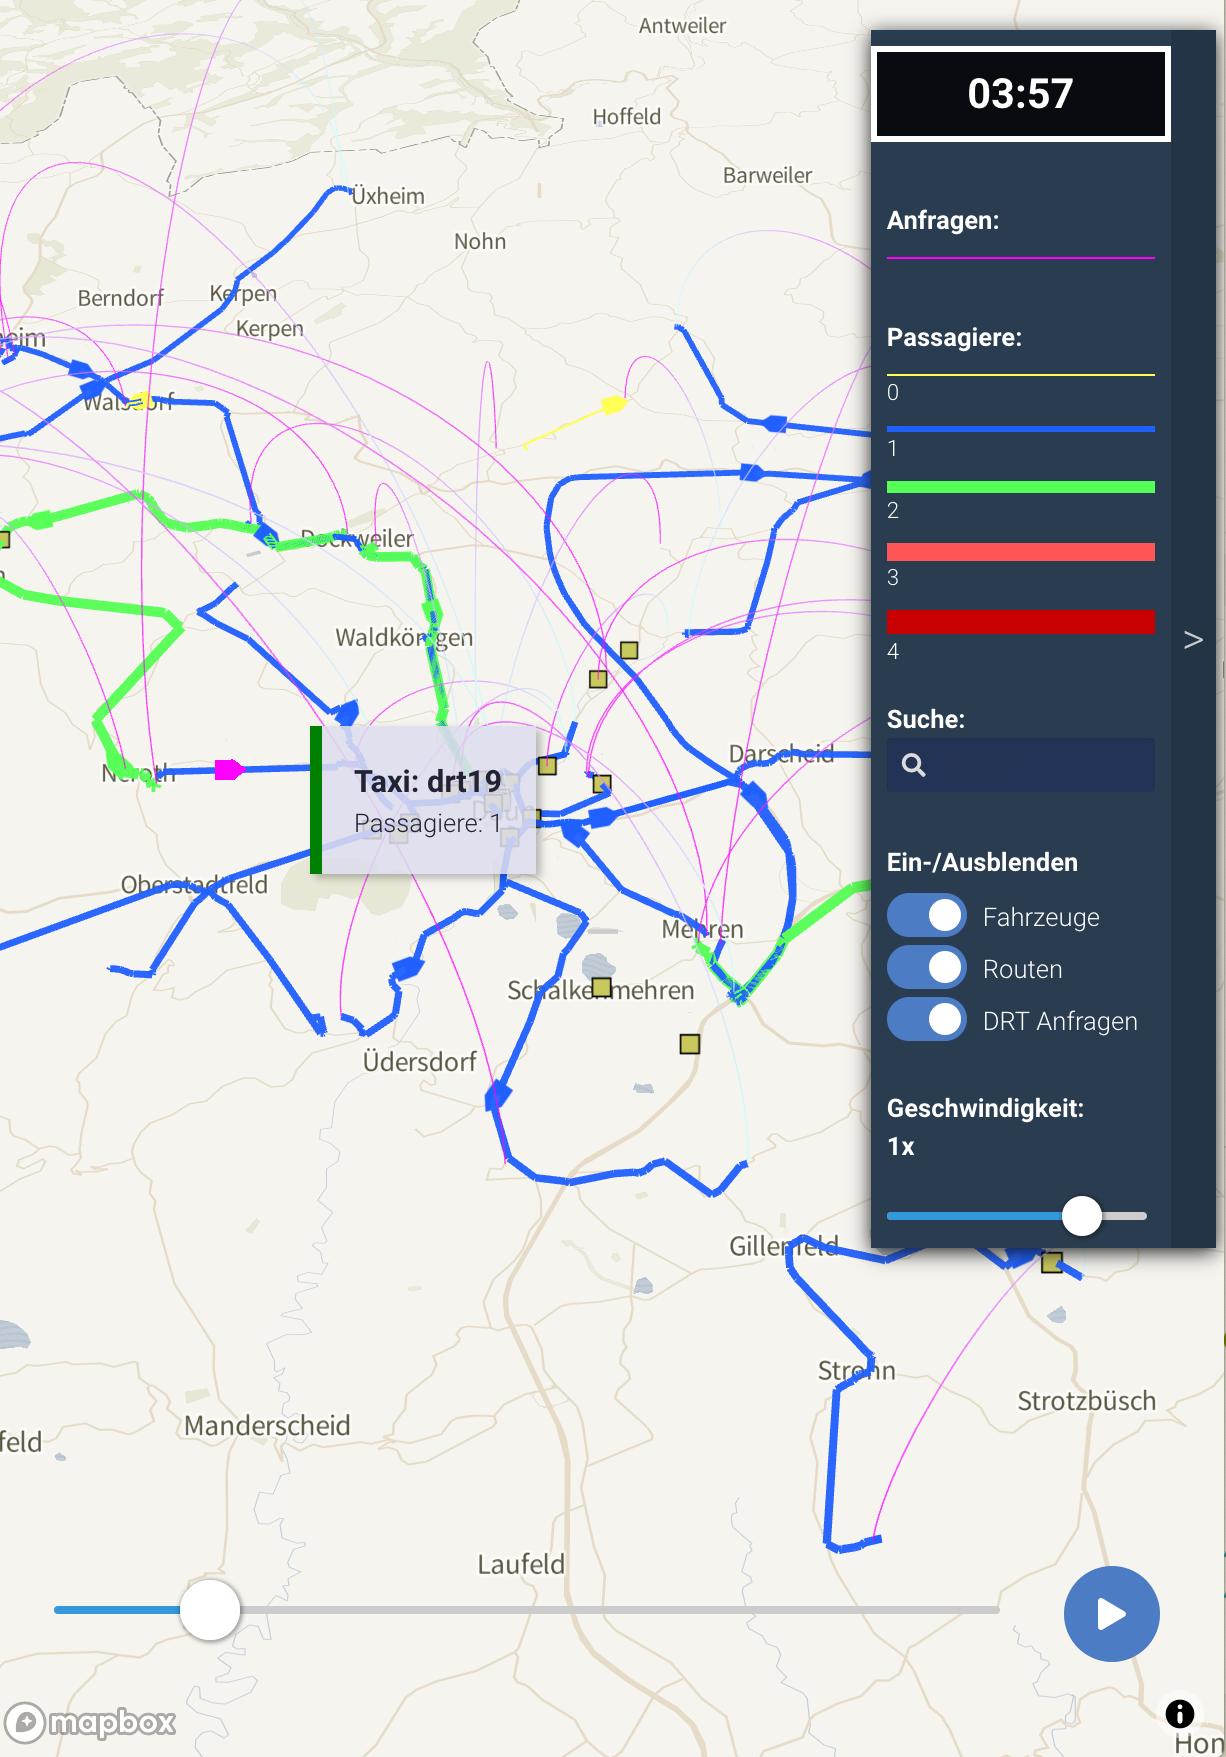
\includegraphics[width=\linewidth]{chapters/22-avov/images/fig-drt-vehicles.png}
   \caption{DRT vehicles and routes}
   \label{fig:avov-drt-vehicles-routes}
\end{minipage}
\begin{minipage}[c]{0.45\textwidth}
   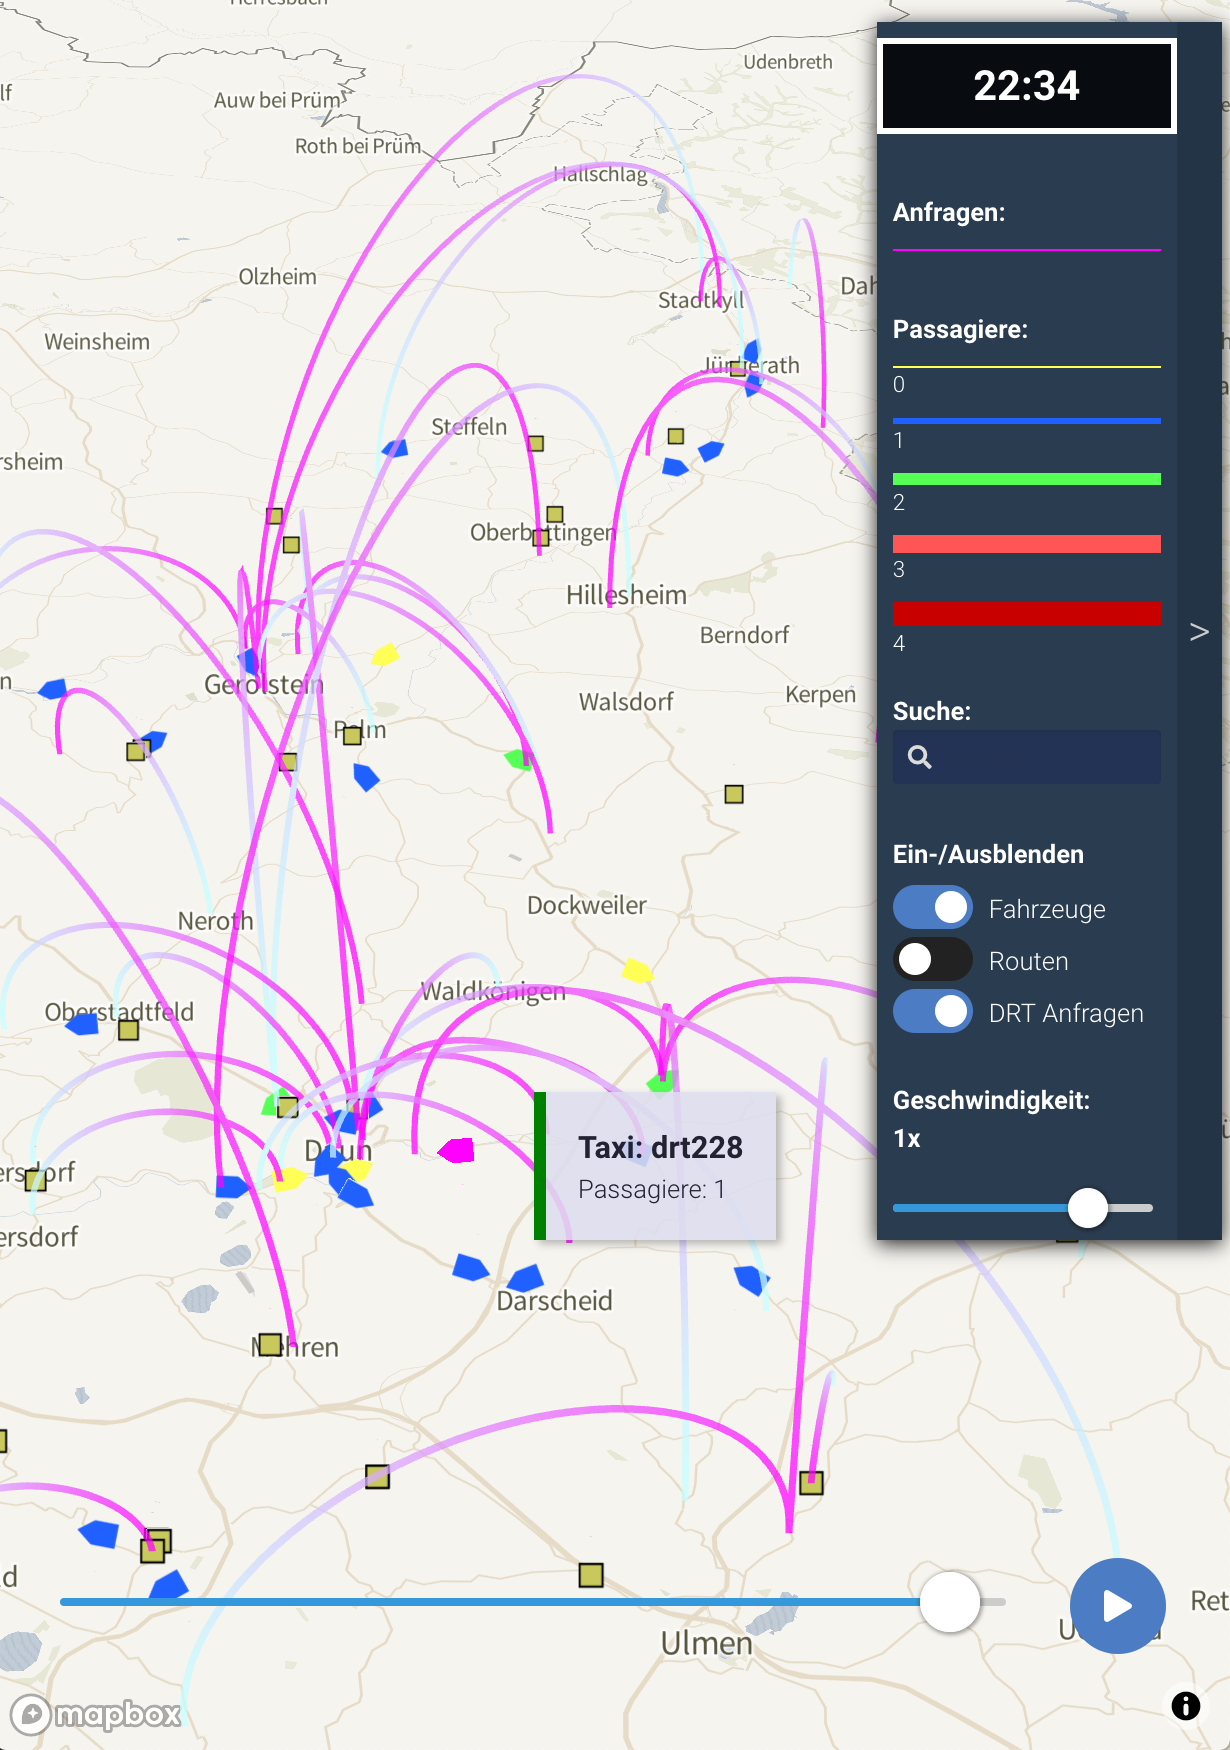
\includegraphics[width=\linewidth]{chapters/22-avov/images/fig-drt-flyovers.png}
   \caption{DRT passenger origins and destinations}
   \label{fig:avov-drt-od}
\end{minipage}
% \caption{Demand Responsive Transport (DRT) animation screenshots}
\end{figure}

% ---------------------------------------------------
\subsection{DRT Passenger and Vehicle volumes}
\label{avov-volumes}

Aggregate summaries of roadway volumes depict total DRT pasenger or vehicle volumes in the entire simulation, or for specific times of day. The user can click on a specific link to see the diurnal (time of day) distribution of trips for that link, or can modify the time window being displayed for all links from total to a specific range, such as 6 A.M. to 9 A.M. if morning commute trips are being studied.

Difference plots compare the DRT scenarios to the "base case" depicting current conditions. Figure \ref{fig:avov-vehicles-daily} shows an example vehicle volume plot, with the width of the links commensurate with volumes on each link.

\begin{figure}[ht]
  \centering
  \begin{minipage}[c]{0.45\textwidth}
     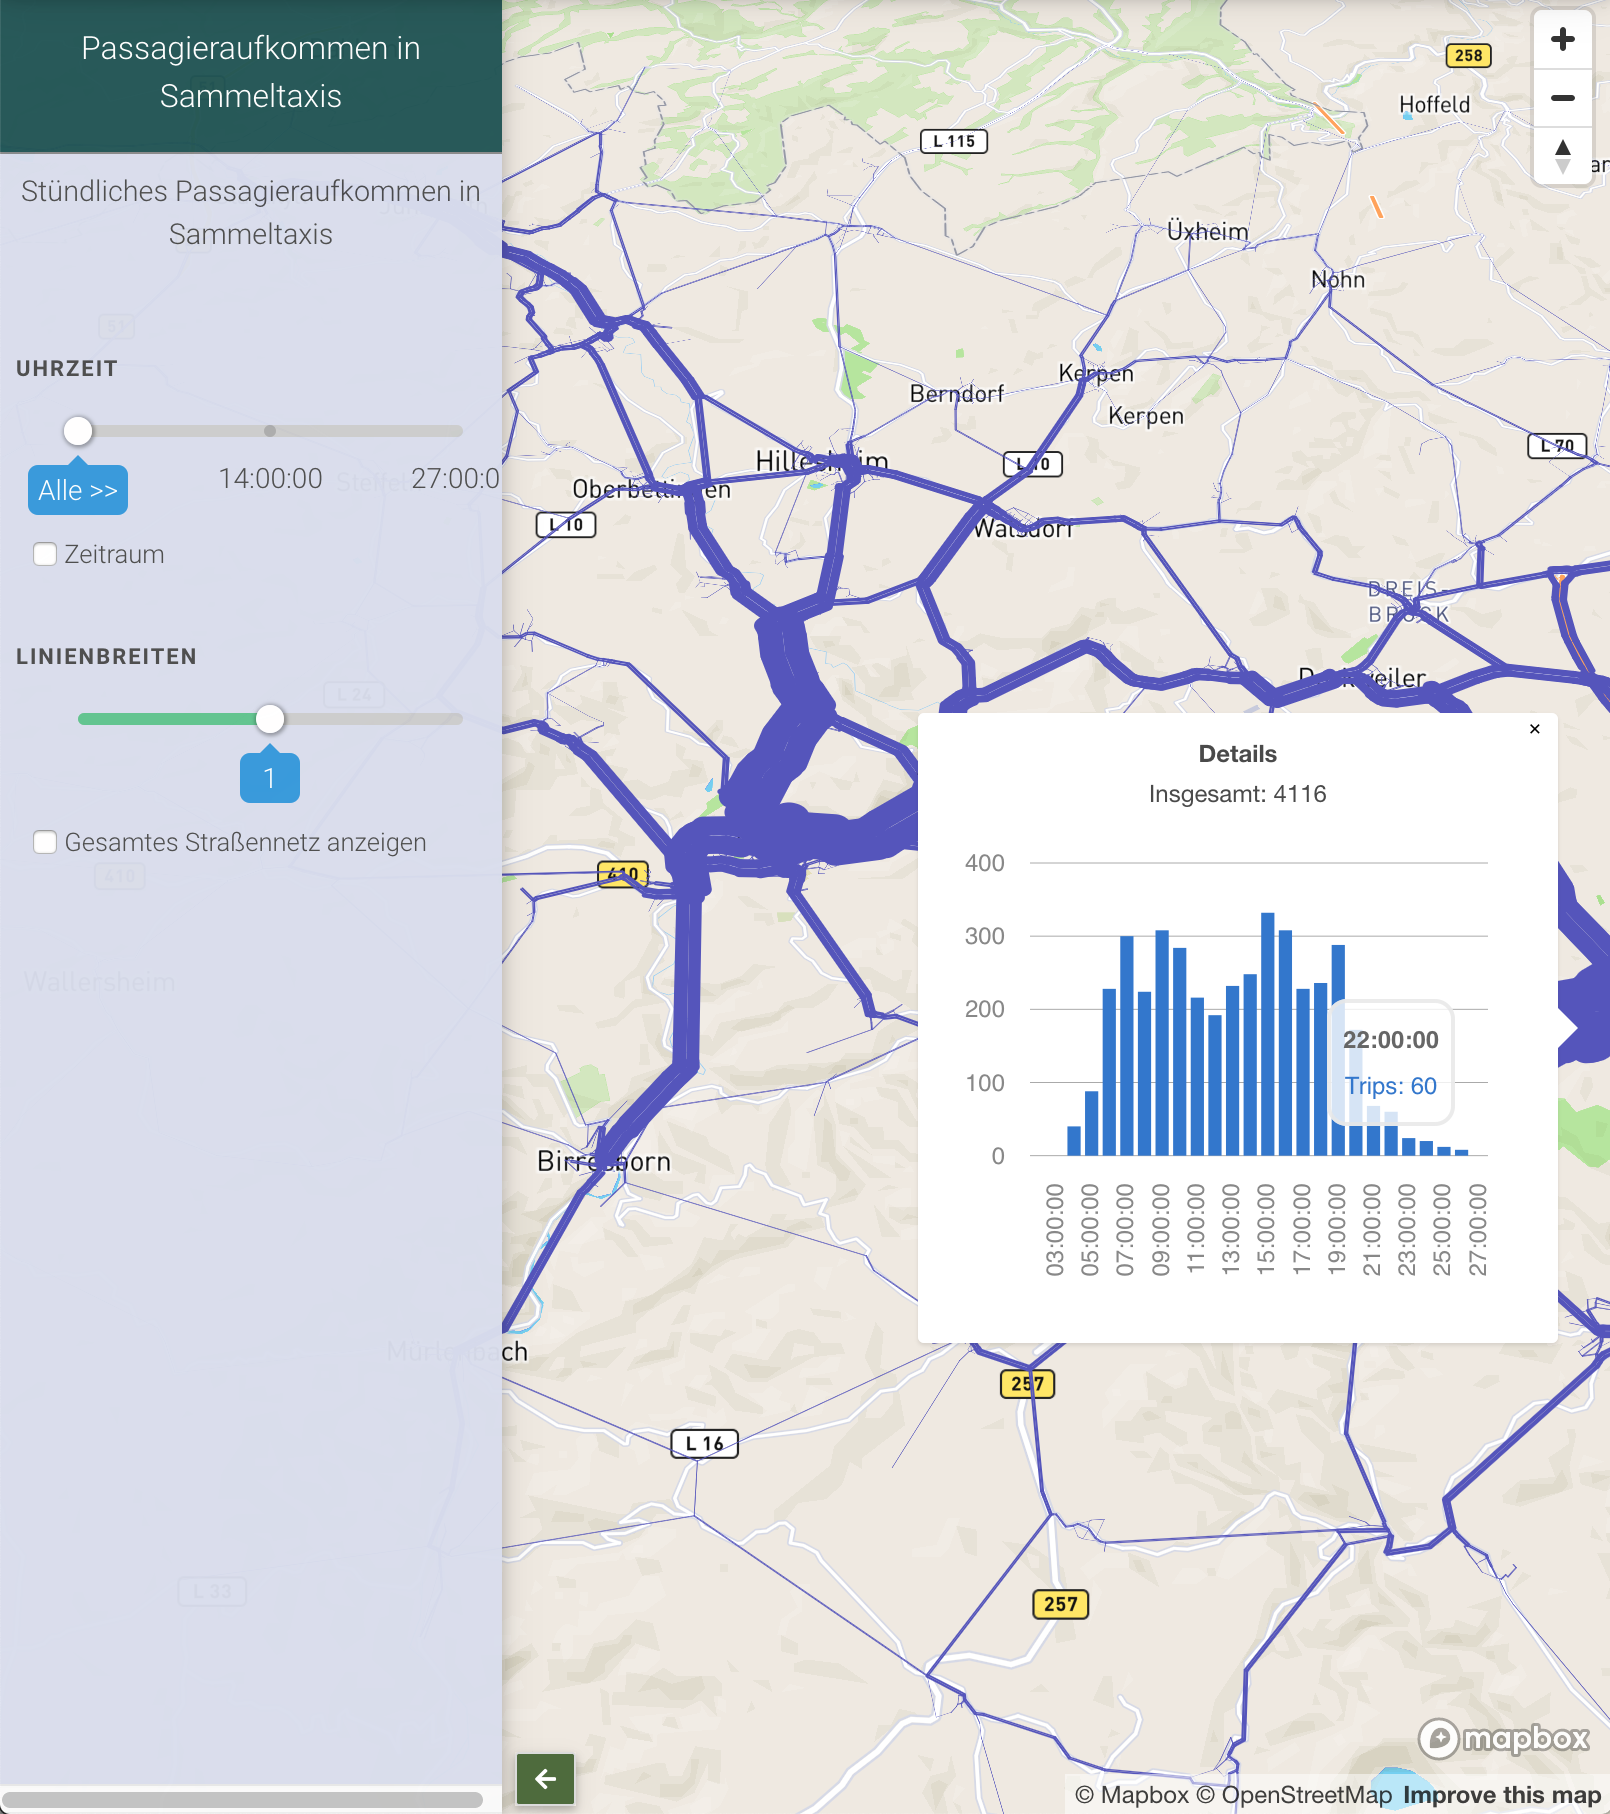
\includegraphics[width=\linewidth]{chapters/22-avov/images/fig-link-vols.png}
     \caption{DRT Vehicle volumes, daily aggregation }
     \label{fig:avov-vehicles-daily}
  \end{minipage}
  \begin{minipage}[c]{0.45\textwidth}
     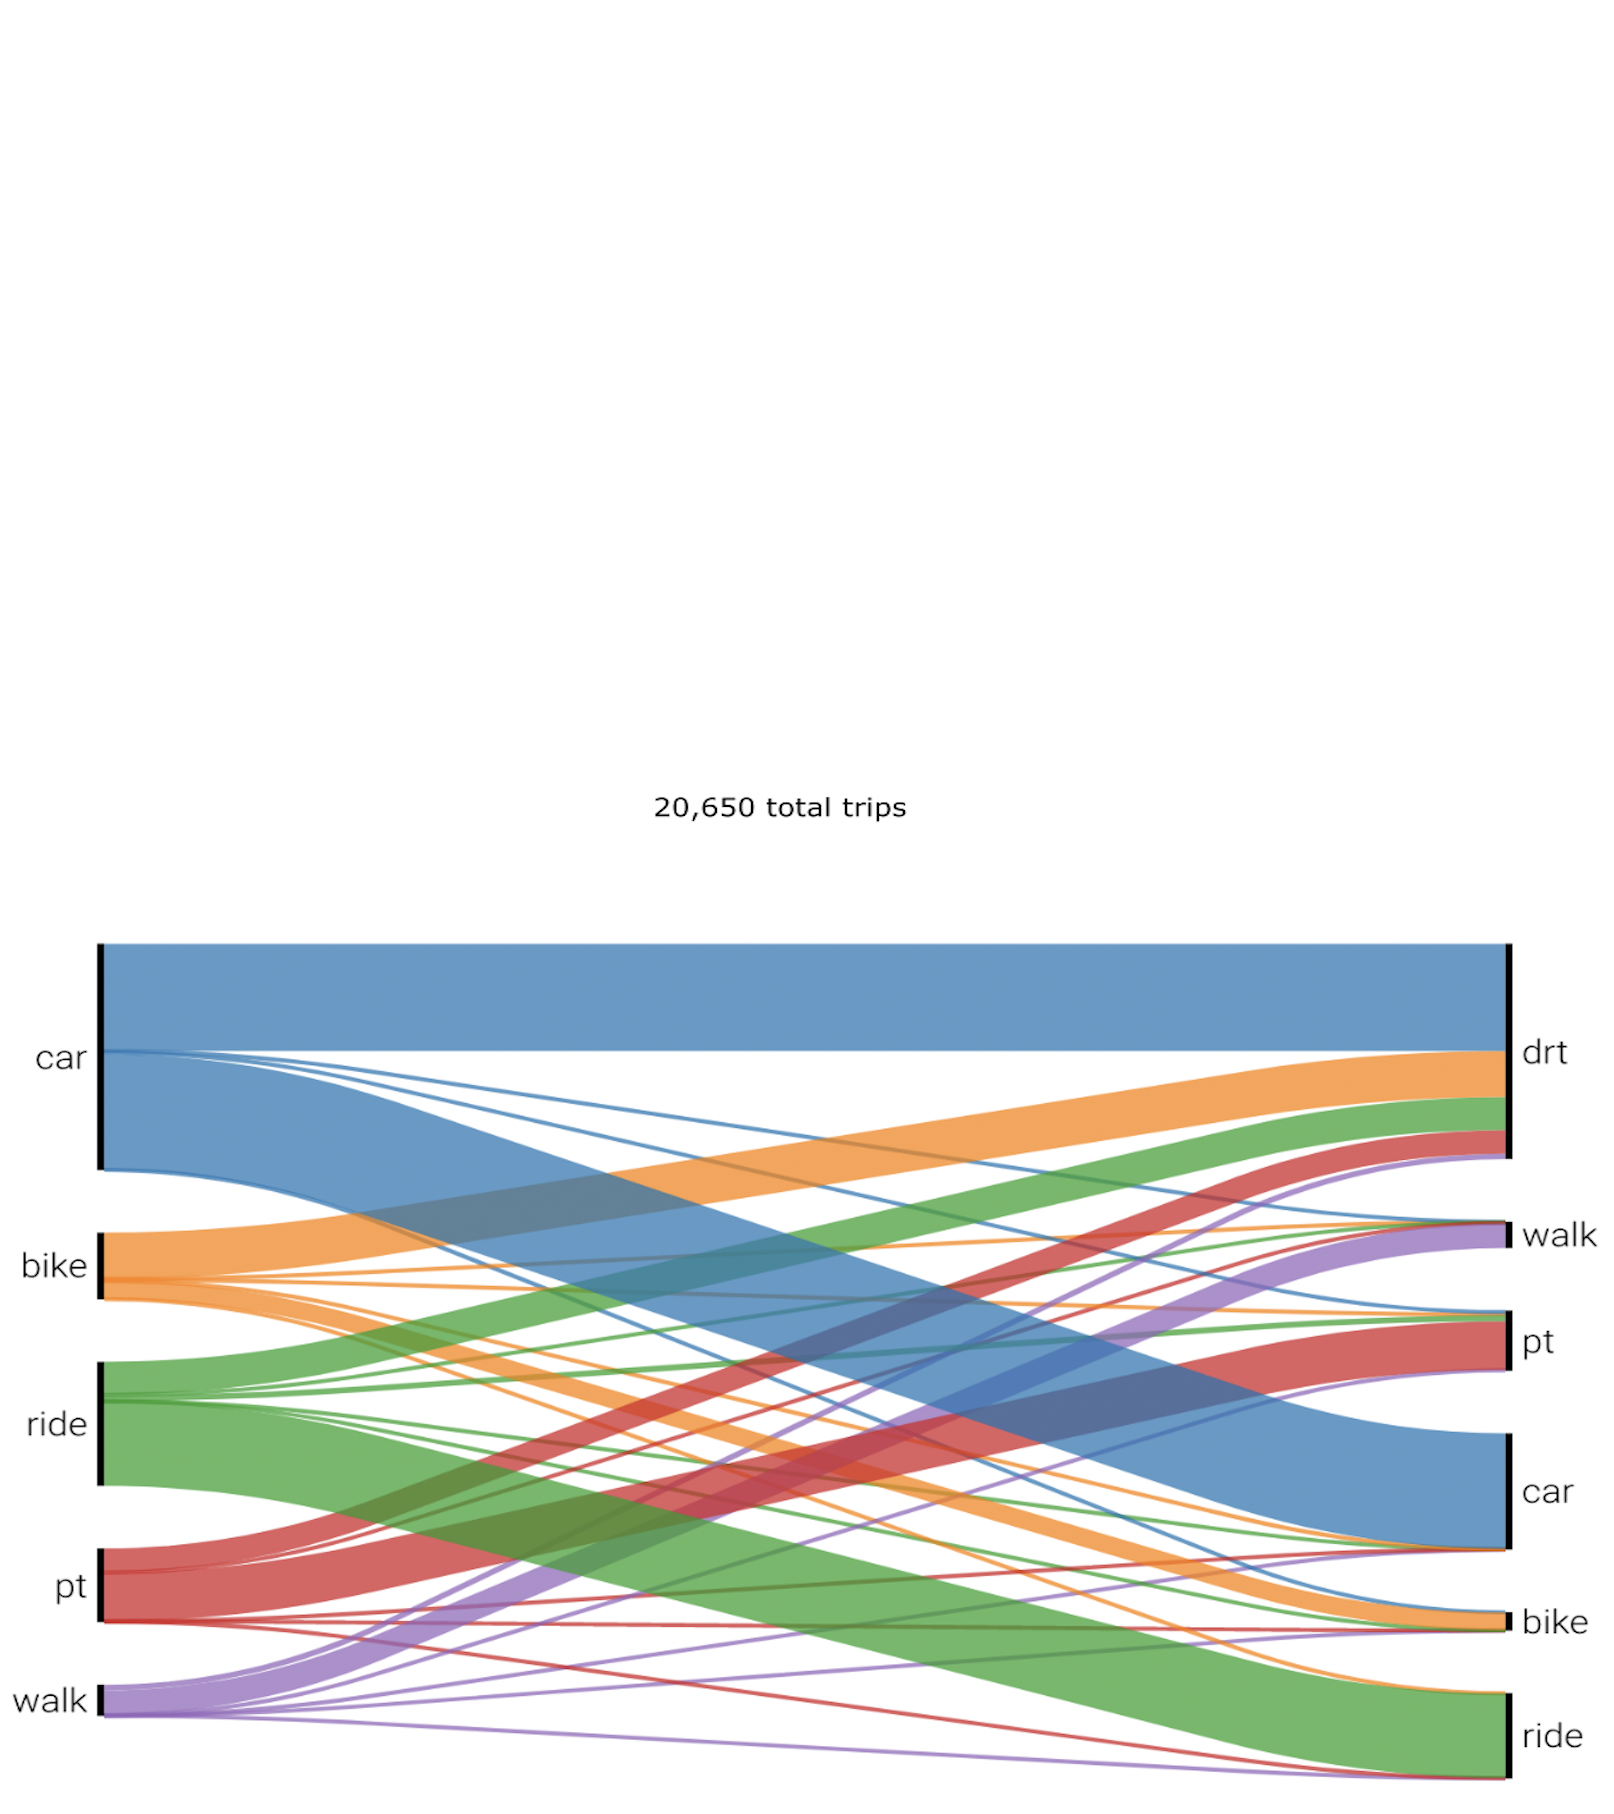
\includegraphics[width=\linewidth]{chapters/22-avov/images/fig-mode-share.png}
     \caption{Mode shift, DRT alternative vs. base case}
     \label{fig:avov-modeshift}
  \end{minipage}
  % \caption{Dynamic Response Transit (DRT) further visualization examples}
\end{figure}

% ---------------------------------------------------
\subsection{Cross-Scenario Modal Shifts}
\label{avov-mode-shifts}

Users can also \emph{compare} the aggregate total mode shift from one scenario to another; in this study comparing DRT scenarios to the base case. These visualizations highlight the degree to which the new DRT mode is "stealing" trips from existing transit and bicycle modes versus from private vehicles. Figure \ref{fig:avov-modeshift} shows an example mode shift diagram.

%% ----- RESULTS -----
\section{Results}
\label{avov-results}

Throughout summer 2020, the team iterated on dozens of DRT scenarios: varying pricing structures, presence of drivers vs. fully automated service, service coverage areas, maximum wait time goals, and so on. In August 2020 began the first public meetings with transit agency staff, with the fully operational website at \href{https://vsp.berlin/avoev}{vsp.berlin/avoev/} (available in German only).

The final site displays a front page listing the results for 6-8 scenarios in each region, covering a wide spectrum of DRT scenarios. Then for each scenario, visualizations include the individual agent animations (see above) with occupancy, origin/destination, and routing details; mode shift summaries vs. base case; vehicle volume, passenger volume, and volume differences on roadway links compared to base case; aggregate levels of tripmaking for trips originating or destined to geographical areas ("hexagon plots"); as well as detailed model output summary graphs depicting general taxi occupancy levels by time of day and more.

Each outreach meeting started with technical staff describing the study, the agent-based model, and the results for each alternative in overview; followed by small break-out groups online, in which people could explore the scenarios and discuss the findings amongs themselves; and finally a return en banc for group discussion. No problems with bugs or site performance were reported.

Some direct feedback from analysts included:

\small{

\begin{displayquote}\emph{
  The DRT viz helped us understand better how the drt code works and find some issues, e.g. when the system is congested weird things can happen and a large group of vehicles with one passenger per vehicle only moves from the same start to the same destination at the same time (in an attempt to save each passenger a few seconds it serves them separately and wastes vehicles which then are missing for the next requests). It is really nice to have requests and vehicle occupancy shown, Via did only the latter after some pre-processing.
}\end{displayquote}

\begin{displayquote}\emph{
  The website obviously made the AVÖV workshops easier. Instead of only sharing our screen we could hand out a website where people could click themselves. Unfortunately it seemed that those listeners did not use the website a lot and rather kept listening to us. Some hypotheses: Maybe because sometimes a group of people shared one computer and their internet connection was bad, maybe because they are not used to that kind of interaction...
}\end{displayquote}

\begin{displayquote}\emph{
  The other plots like passengers/link or vehicles/link are not entirely new; some used QGis to produce those. However, the website forced us to actually produce all those plots systematically instead of 'we could do that plot, but maybe it's not necessary, let's look into something else or raw data only to avoid the hassle of setting up QGis...'
}\end{displayquote}

}

The feedback that some of these visualizations are not entirely "new" is expected: tools such as QGis and Via provide some very nice visualization capabilities already. They are not online tools, however, and are not accessible to non-technical staff such as at a public outreach meeting.

Given this feedback, the initial roll-out of the visualization platform seems to have had a positive impact, and the team expects to continue developing it for further analysis of dynamic-response transit systems.

%% ----- CONCLUSIONS -----
\section{Summary}
\label{avov-summary}

Several years of trial and error led us to this specific combination of technologies and techniques. The research team is deeply indebted to the developers of so many components and libraries on which this is based, all of which are freely available online and without which this work would have been entirely impossible. The final product is more than parts merely cobbled together: a usable, useful tool for decision-making now exists, and the DRT-specific extensions serve as a template for further work.

Paraphrasing Dennis Ritchie's early description of the UNIX system in \citet{Ritchie1978unix}, ``Success lies not so much in new inventions but rather in the full exploitation of a carefully selected set of fertile ideas, and especially in showing that they can be keys to the implementation of a small yet powerful system.''

The successful experience using the platform in a public outreach setting confirms the team's expectation that advanced agent-based simulations can be part of a decision framework and public policy discussions -- ultimately leading to better-informed decisionmaking.

Further enhancements to the underlying platform and to the DRT visualization capabilities are ongoing; the plugin architecture enables other JavaScript developers to write plugins for their own agent-based models and their own use cases, if they so desire.

The website remains online at \href{https://vsp.berlin/avoev/}{vsp.berlin/avoev/}. All code is available at \href{https://github.com/matsim-vsp/avoev}{github.com/matsim-vsp/avoev/} and is licensed under the GNU GPL Version 3 \cite{FSF2007GnuGPL}. As primary author of all of the code therein, I welcome feedback and code contributions.

\section{Acknowledgements}
This research benefited from many discussions with Professor Kai Nagel, and was funded in part by the German Federal Ministry of Transport and Digital Infrastructure (funding number 16AVF2160)


\chapter{PAVE: Data visualization for analyzing the potential of automated transport systems}
\label{ch:pave}
%% ----- INTRODUCTION -----
\section{Introduction}
\label{pave-intro}

Building on the initial success of COVID-Sim and the subsequent AVOEV project website described in Chapter \ref{ch:avov}, this chapter describes a third and final project-specific website built using the same combination of curated runs stored on a file server, with a custom front-end website. This project website was intended to be outward-facing, for public outreach meetings with government agencies and the wider public audience, rather than an internal-facing analyst tool.

%% ----- PROJECT DESCRIPTION -----
\section{Project Description}
\label{pave-project-description}

The \gls{PAVE} project is studying the ``Potential of Automated Transport Systems'' in Berlin, Germany, and is sponsored by a consortium of multiple universities and private firms in Germany.\footnote{To learn more about the PAVE Project and PAVE Consortium, see the main PAVE website at \href{https://pave-your-way.de}{pave-your-way.de}}

The project is exploring several demand-responsive transport (\gls{DRT}) configurations including automated taxi service (``Robotaxi''), automated, pooled shuttle service (``Pooling''), combinations of these services, as well as a strict ban on non-DRT private vehicles inside the study area. Multiple study areas, cost structures, fleet sizes, and several other parameters are studied.

\subsection{DRT scenarios being studied}
\label{pave-scenarios}

While the study details themselves are not critical, a basic overview of the scenarios being tested testing is helpful to understand how the data visualizations for the project website are constructed.

These four main scenarios are being considered:

\textbf{Robotaxi.} In this scenario, one passenger at a time can be transported by each DRT vehicle. The DRT provider aims to minimize the needed subsidy (or maximize profit) while trying to hold 95 percent of wait times to 7 minutes or below; this can be seen as a regulatory constraint. The simulation was used to approximate the resulting demand and the necessary fleet size for several cost structure alternatives at a rough planning level.

\textbf{Pooling.} In this scenario, multiple passengers can be transported by each DRT vehicle simultaneously. In this scenario the DRT provider also aims to minimize the needed subsidy need (or maximize profit),  while trying to keep 95 percent of wait times below 7 minutes. The simulation was used to approximate the fleet size needed and the resulting demand for various user prices. The base fare is paid per ride; the price per km is paid for the direct distance when booking the ride. When several passengers get pooled the actual travelled distance may differ.

\textbf{Combined.} In this scenario, travelers can choose between both mobility-on-demand modes of operation. The ``robotaxi'' service is operated within the inner core of Berlin, while the pooling service area covers the entire city. The taxi operator is more expensive as it guarantees direct transportation. As in Scenarios 1 and 2, the simulation approximated the resulting demand and necessary fleet sizes, but in this case for both operators in competition with each other.

\textbf{Ban private vehicles.} In this scenario, private cars are banned from the inner core of Berlin. As a substitute, a DRT system is introduced. People can transfer from their private cars to the DRT system and vice-versa, which happens at the border of the car-free zone. No regulatory waiting time threshold is assumed in this scenario.

%% ----- UNIQUE SITE FEATURES -------------------------------
\section{Supporting decisingmaking with an interactive website}
\label{pave-site-features}

To support the public outreach meetings for the PAVE project, a third project-specific website was built using a similar technology stack as for the previously described COVID-Sim and AVOEV projects. As the purpose was to build something that agency staff and the genuine public could use, a much larger effort was spent on honing the user interface and usability of the site; for example, paying more attention to creating a pleasing layout and a consistent color palette, and also including explanatory text where needed to avoid overly technical jargon.

Roadway volume plots, simulated DRT vehicle animations, and mode shift charts similar to those used in the AVOEV project were implemented for the PAVE website. These are described in sections \ref{avov-drtviz} and \ref{avov-volumes}.

Some new and updated components were built, and these are described below.

%% ----- -----------------------------------
\subsection{Scenario chooser}
\label{pave-scenario-chooser}

Building on the multivariate COVID-Sim simulation result picker described in section \ref{covid-single-page-application}, a new scenario chooser was built for PAVE. An iterative design process, working closely with the analyst team, led to the final layout and behavior. Large graphical elements depicted the different service areas on a map, along with buttons for selecting differing fare structures. The user could essentially browse and select from the various scenarios shown on a left-side navigation panel, and the results for that scenario would immediately appear in the main window pane.

Figure \ref{fig:pave-scenario-chooser} shows a close-up of a typical scenario output page, with the scenario selector on the left side and the various outputs to the right. These are explained in more detail below.

\begin{figure}[ht]
  \centering
  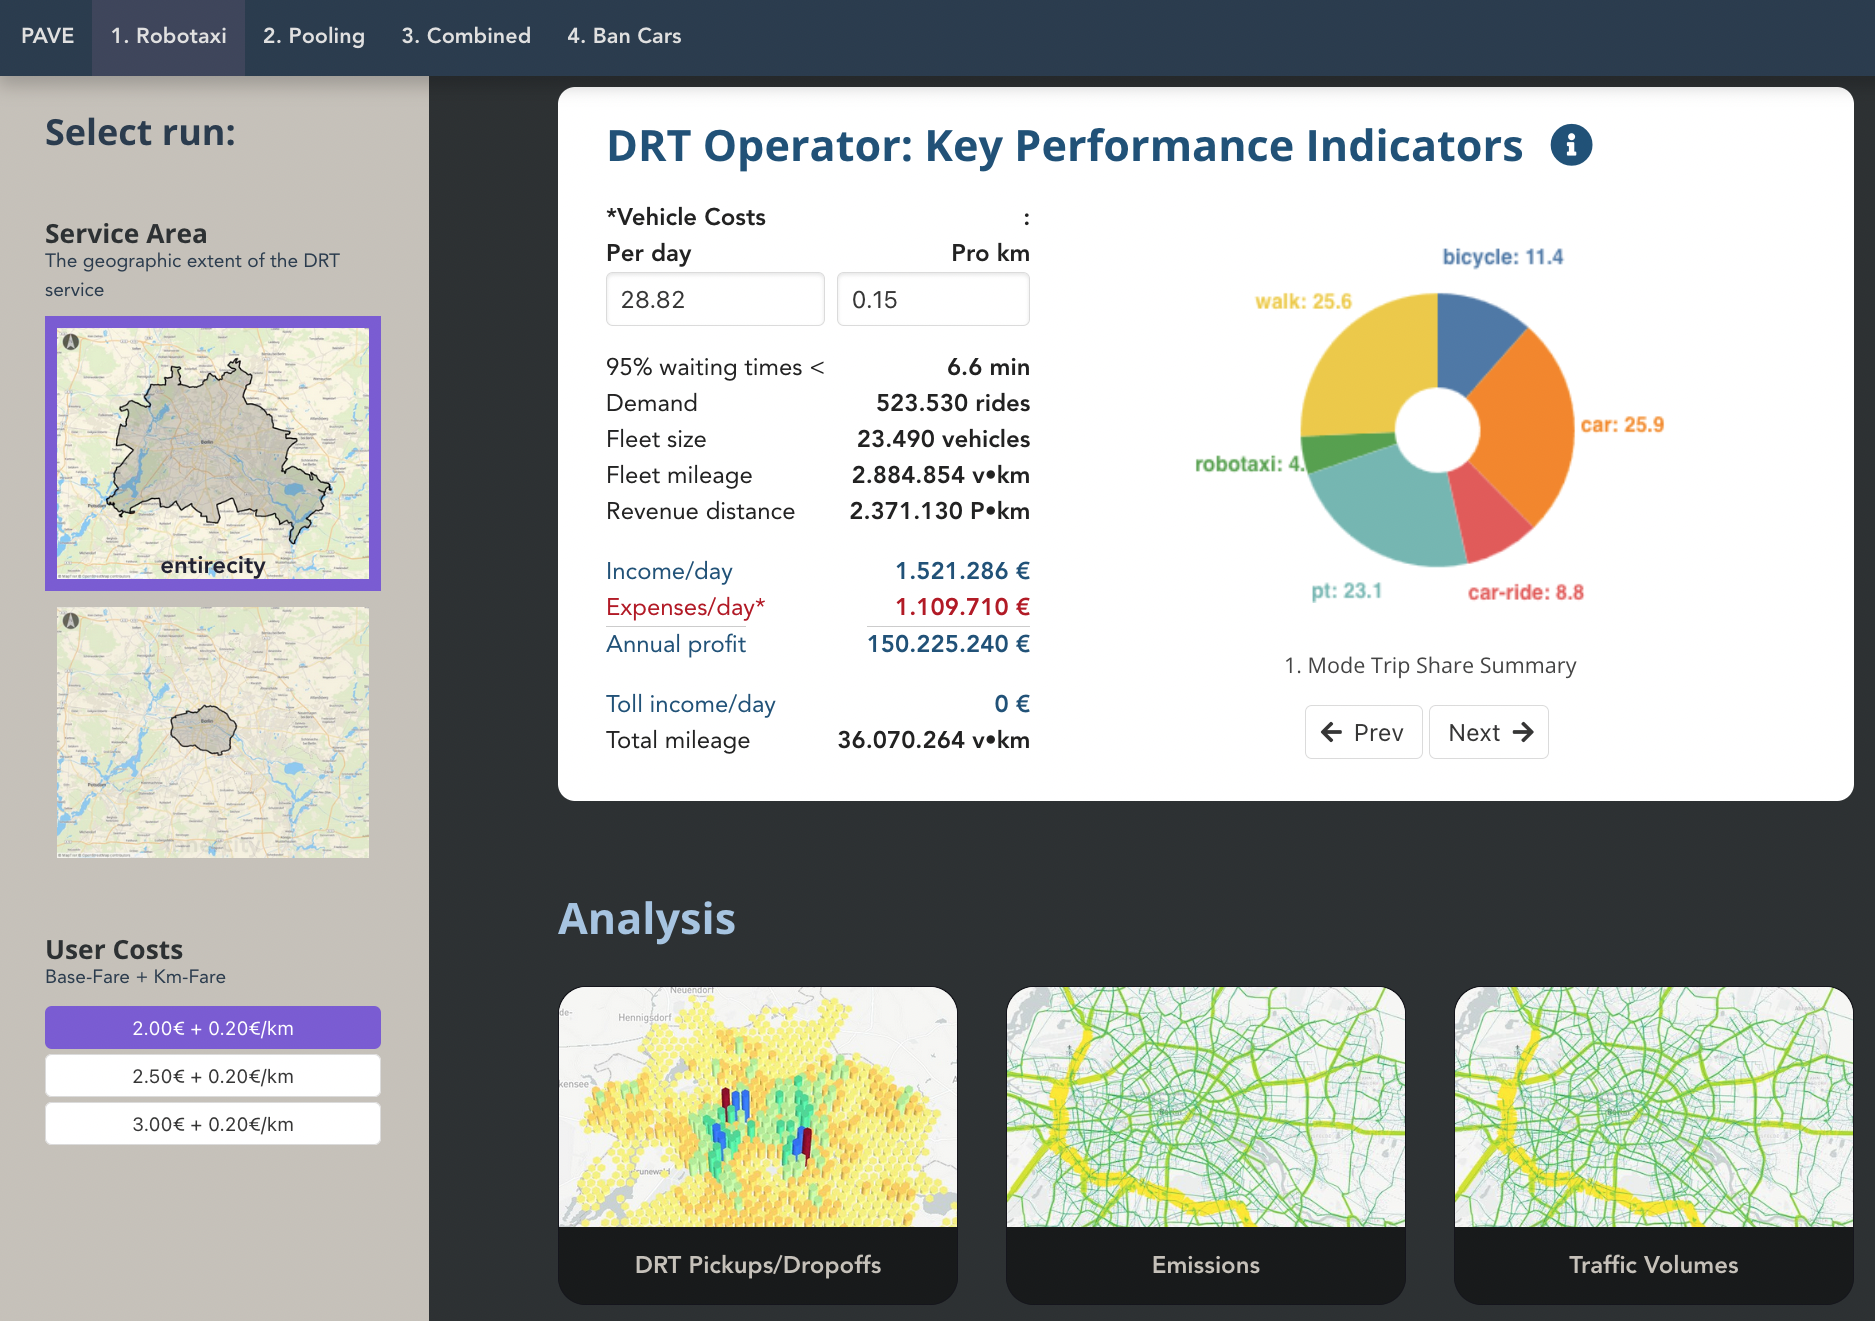
\includegraphics[width=0.95\linewidth]{chapters/23-pave/images/fig-kpi-panel.png}
  \caption{Screenshot of PAVE scenario viewer, with left-side selector and key performance indicators and visualizations on the right}
  \label{fig:pave-scenario-chooser}
\end{figure}

%% ----- -----------------------------------
\subsection{Key performance indicator panel}
\label{pave-kpi-panel}

A new summary \gls{KPI} panel provided top-level summary statistics for the selected scenario. This panel went through many rounds of revision with the analyst team and project partners before settling on the final set of KPIs. The panel includes aggregate statistics including total demand, fleet size, fleet mileage, operator income and expenses, and also includes a ``carousel'' of mode share and mode shift diagrams which the user can scroll through.

This KPI panel also includes interactive text entry fields for vehicle costs, both per-vehicle and per-km, so that users can explore the consequences of different cost parameters if they desire. Default values are used initially, but any cost parameters can be tested in this manner

Figure \ref{fig:pave-scenario-chooser} includes an example of the KPI panel.

%% ----- -----------------------------------
\subsection{Interactive DRT animation}
\label{pave-drt-animation}

The DRT animation plugin from the AVOEV project (see Section \ref{avov-drtviz}) was updated and improved for the PAVE project. Much larger simulation support was added, as the PAVE project encompasses the capital city of Berlin instead of less-populated rural areas of Germany, as in AVOEV.

This support was enabled by use of the JavaScript \emph{crossfilter} library.\footnote{Crossfilter is available online at \href{https://crossfilter.github.io/crossfilter/}{crossfilter.github.io/crossfilter/}} Crossfilter allows filtering and exploring of large multivariate datasets, and supports extremely fast (measured in milliseconds) interaction with coordinated views, even with datasets containing millions of records. Crossfilter takes advantage of the fact that most user interactions only modify a single dimension at a time (in this case the elapsed time of the simulation), which requires only small adjustments to filter values. Incremental filtering and reducing is significantly faster than starting from scratch. Crossfilter uses sorted numerical indexes, dramatically increasing perfor­mance over other sorting and filtering techniques.

With this library, the vehicle position dataset can be filtered to include only the exact second of the simulation that is currently displayed, and then only those filtered vehicle trace segments are painted on the screen. Up to tens of thousands of vehicles can be simultaneously animated in the browser using this technique.

For example screenshots of the DRT animation, refer to Figure \ref{fig:avov-drt-vehicles-routes}.

Note that for even larger datasets, crossfilter was no longer sufficient and more direct graphical methods using \gls{GPU} accelerated techniques were required. Those techniques are addressed in Chapter \ref{ch:simwrapper}.

%% ----- -----------------------------------
\subsection{Aggregate DRT origin/destination patterns}
\label{pave-od-hexagons}

An aggregate summary of the origin and destination locations of DRT trips was also created to help show the ``big picture'' of how DRT was being used in the study area; individual vehicle animations described above are very visually pleasing but do not provide a comprehensive systemic depiction.

Often, this type of aggregate summary data is collected into districts or analysis ``zones'' that are predetermined by analysts. For this visualization, a fully interactive plot was implemented consisting of hexagonal areas equally distributed across the study area; and the size of the hexagons themselves is user-selectable with a simple slider.

The hexagon plot aggregates either total DRT trips originating or destined for points inside each hexagon; the aggregation is then colored from pale to dark to emphasize areas with large numbers of DRT trips. A three-dimensional view is also possible, with the total aggregate value mapped to the height of hexagonal ``cylinders'' on the map.

An example of this hexagon-area-based DRT trip aggregation is shown in Figure \ref{fig:pave-xy-origins}, showing an example of total DRT trip origins.

\begin{figure}[ht]
\centering
  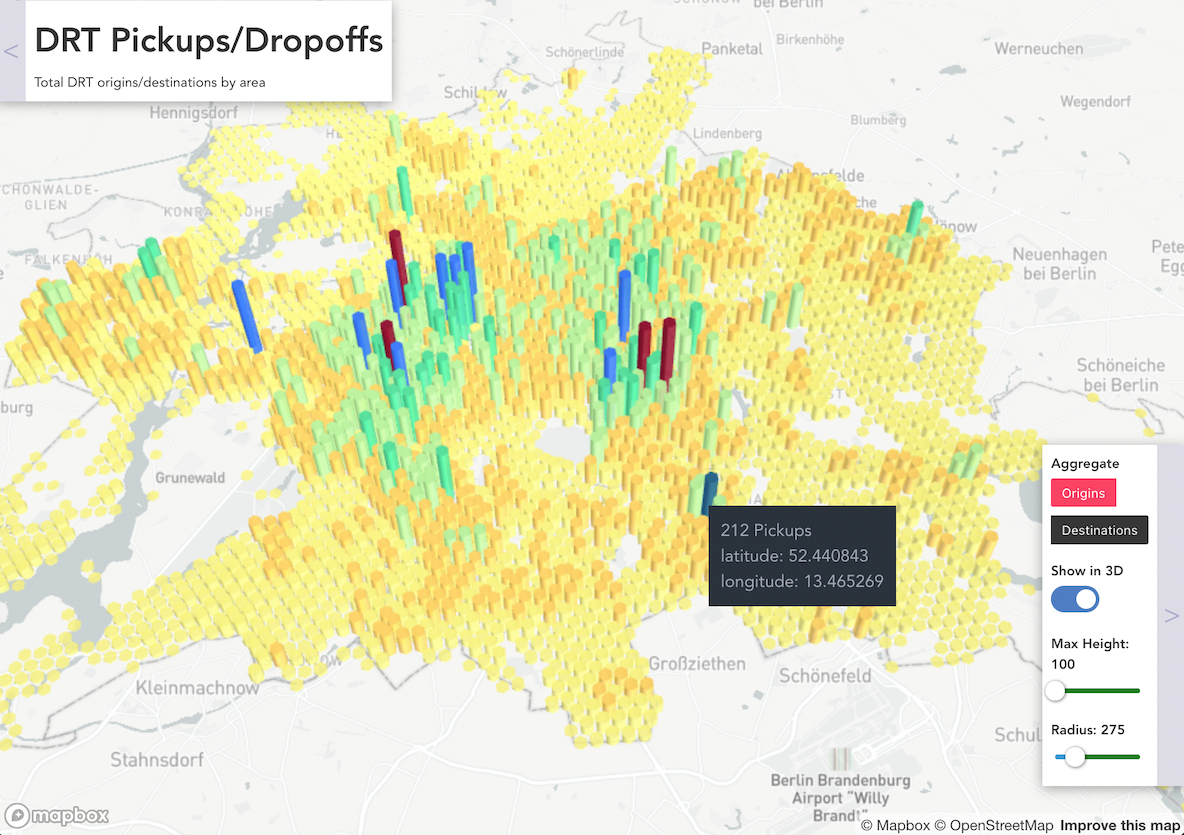
\includegraphics[width=0.95\linewidth]{chapters/23-pave/images/fig-xy-origins.png}
\caption{PAVE aggregate summary of DRT trip origins for an example scenario. Color and height represent the total number of trips in an area, and the user can hover over an area to see the precise number of trips.}
\label{fig:pave-xy-origins}
\end{figure}

%% ----- FEEDBACK -----
\section{Public Outreach Results and Feedback}
\label{pave-feedback}

The website was introduced to consortium partners and was presented to the public in multiple public outreach meetings in Berlin during spring 2021. Staff used the site to explain to the public how the different scenarios were configured, and then participants were given the opportunity to explore the site on their own, while also examining more traditional outreach materials including handouts and posters.

Feedback from staff was generally positive: one team member stated, ``I think people liked it. But mostly they wanted to talk to us about the different scenarios and interact with us directly, instead of using the website.''

%% ----- DISCUSSION AND OUTLOOK -----
\section{Discussion and Outlook}
\label{pave-discussion}

As the visualization platform for these project websites grows in capability, its usefulness to analysts grows as well. However, the level of effort to produce a website portal for this one small project was notably high: the site was built over the course of three months and many hours were spent making small modifications on an iterative basis. Some new components that were developed have potential to be used in future projects, but that would require that the components be made in a more modular fashion that is not tied to specific project outputs.

Overall, the built site was well-received in the public outreach sessions and was well-liked by analyst staff. To truly inform the public and the decisionmaking process requires more than pleasing maps or a nice website, but it did appear to have a positive impact on discussions, however small.

The PAVE project was the third project site built on a common foundation of web-based visualization technologies and HTTP-accessible file storage for site configuration and simulation outputs. Several novel components were built for the project, including visual navigation for scenario selection, a consistent key performance indicator output panel, three-dimensional interactive display of trip origin and destination patterns, and a carousel for collating related charts in order to reduce visual clutter.

Feedback from users was positive. Internal staff considered the website well-conceived, but the level of effort to produce this bespoke site was higher than desired. This led to questions and suggestions that the features might be better integrated in a more general platform instead of creating additional project-specific websites. The development of a generic data visualization platform in this vein is the subject of the following chapters, in Part III.


% =============================================================================
% PART III: A GENERALIZED BROWSER-BASED DATA VISUALIZATION PLATFORM:
%           Supporting analysts and decisionmakers with a configurable platform
% =============================================================================

\part{Part 3: A Generalized Browser-Based Data Visualization Platform}
\label{part:3simwrapper}

\chapter{SimWrapper: a browser-based data visualization platform for microsimulation outputs}
\label{ch:simwrapper}
% ------------------------------------------------------------------------------------
% # Chapter: SimWrapper
% ------------------------------------------------------------------------------------

Having confirmed the utility and capabilities of a fully browser-based
data visualization approach for three individual project portals, we
then set out to generalize the method. An entirely generic data
visualization platform is inherently more difficult than a project
portal, as every researcher investigates widely disparate questions and
will be focusing on completely different outputs. Where one researcher
may be using MATSim to predict future dynamic-response shared taxi
vehicle flows, another is doing emergency-response evacuation planning,
or emissions reduction through increased transit ridership efforts. The
tool needs to be extremely flexible.

% \begin{figure}
%   \centering
% 	\begin{minipage}{.75\textwidth}
% 		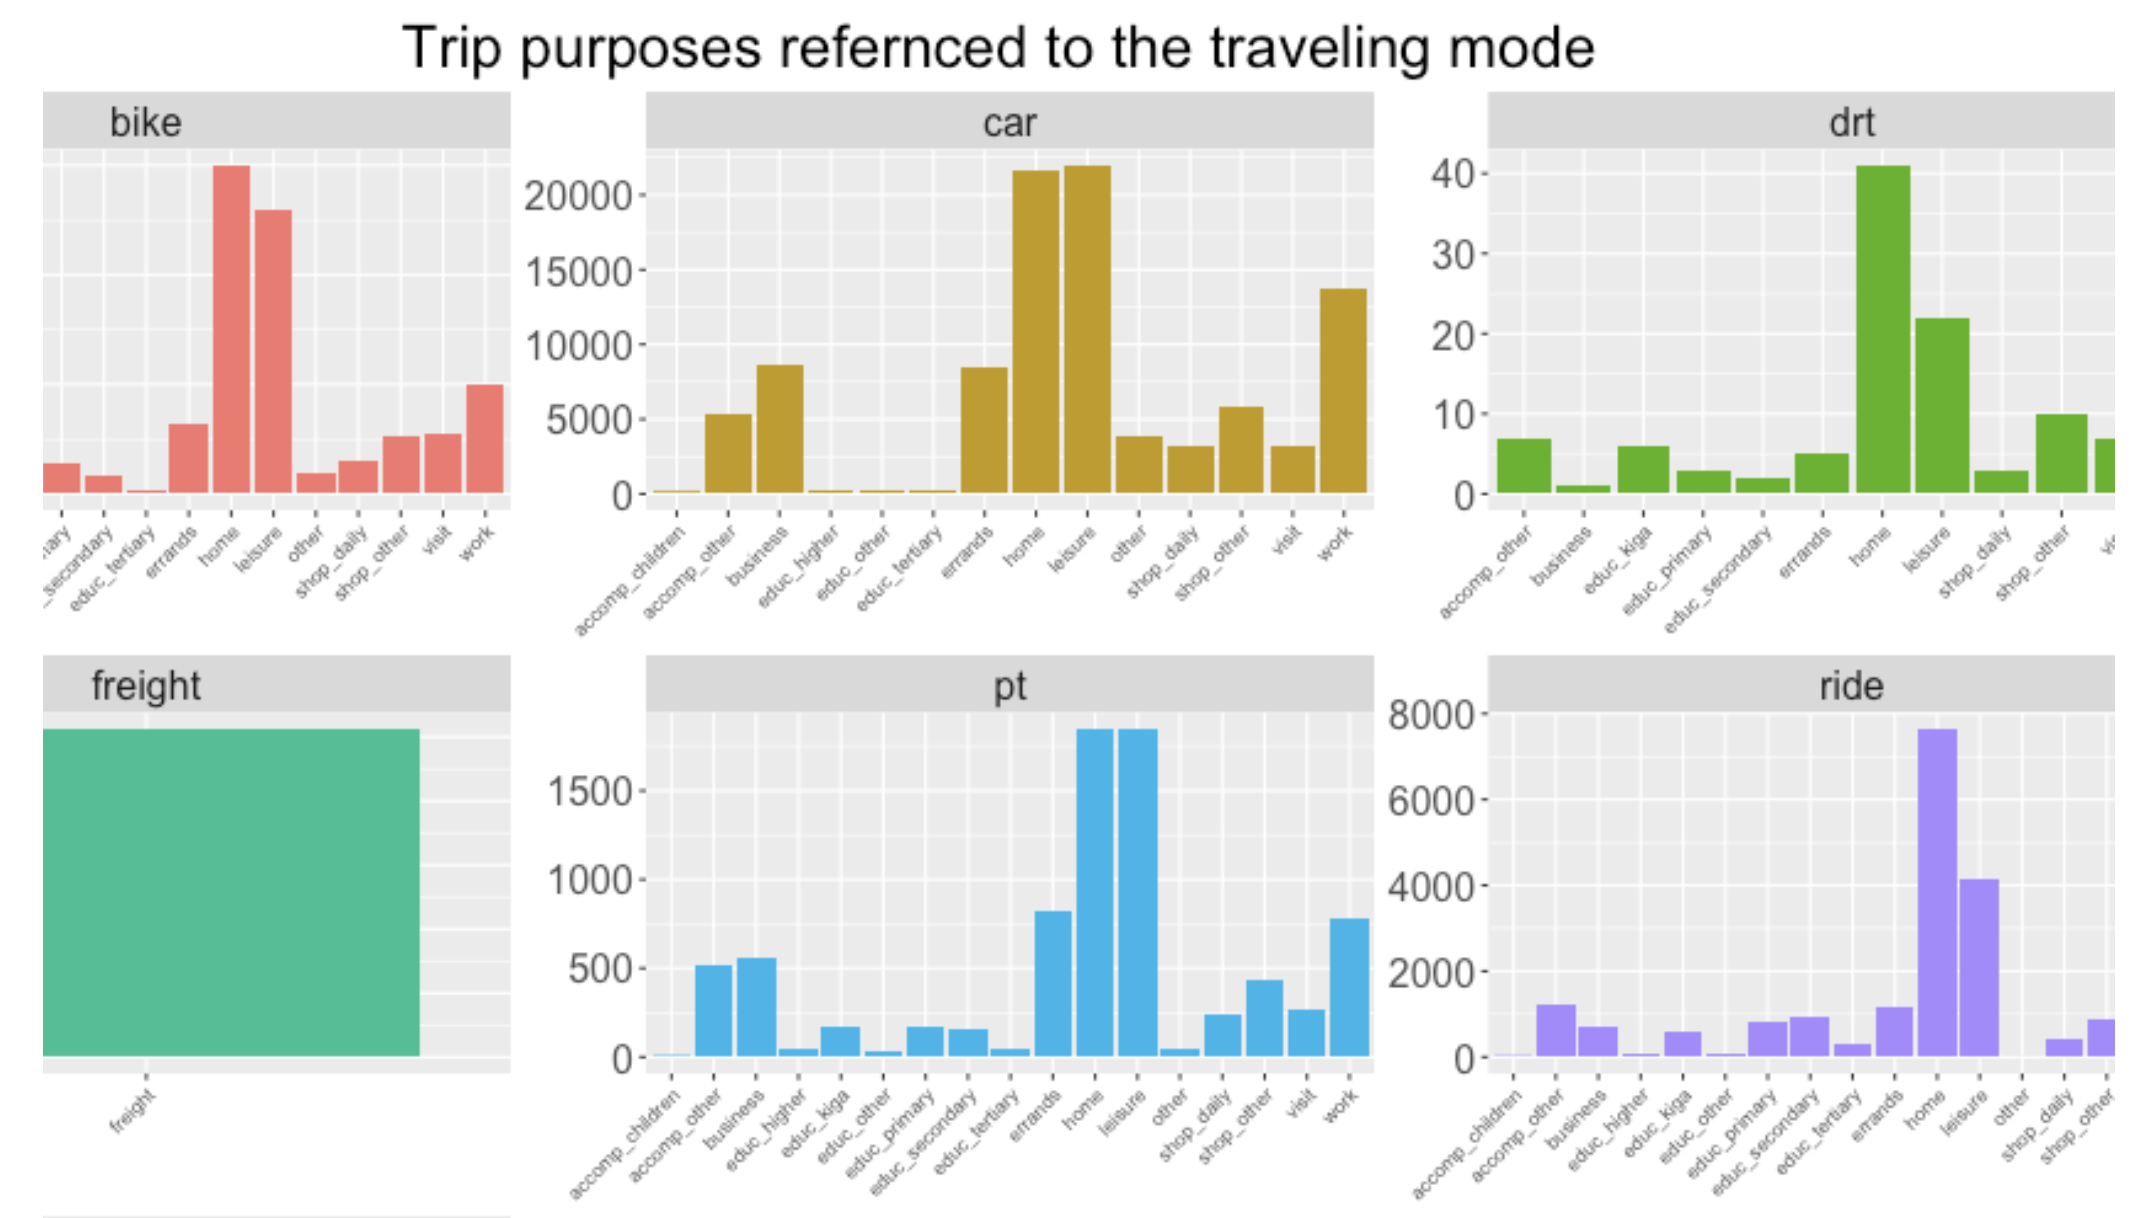
\includegraphics[width=\textwidth]{chapters/06-simwrapper/images/charts.png.pdf}
% 		\caption{CHart: stuff.}
% 		\label{fig:chartychart}
% 	\end{minipage}
% \end{figure}

This chapter describes \textbf{SimWrapper}, an open-source web-based
data visualization platform we developed with the goal that it be useful
for anyone working with MATSim outputs or even outputs from other
data-intensive microsimulation models.

% ------------------------------------------------------------------------------------
% ## SimWrapper in a Nutshell
% ------------------------------------------------------------------------------------

\hypertarget{overview-simwrapper-in-a-nutshell}{%
\section{Overview: SimWrapper, in a
nutshell}\label{overview-simwrapper-in-a-nutshell}}

Many design questions were already settled in the aforementioned
research YY.

SimWrapper, in a nutshell:

\begin{itemize}
\item
  \begin{enumerate}
  \def\labelenumi{(\arabic{enumi})}
  \item
    is a static website that runs client-side javascript in the form of
    a ``single page application'', a common approach in current web
    development that is compatible with all modern web browsers;
  \end{enumerate}
\item
  \begin{enumerate}
  \def\labelenumi{(\arabic{enumi})}
  \setcounter{enumi}{1}
  \item
    supports network-based file storage for public- and/or
    group-accessible shared data files (model runs), but has no other
    back-end server requirements and can run completely locally if no
    network file storage is available or needed;
  \end{enumerate}
\item
  \begin{enumerate}
  \def\labelenumi{(\arabic{enumi})}
  \setcounter{enumi}{2}
  \item
    allows the user to navigate through their local filesystem or shared
    network storage of model runs to view results that are saved in a
    specific folder, rather than a database-centric approach. This
    matches the design of MATSim and other simulation models which
    produce collections of output files by default;
  \end{enumerate}
\item
  \begin{enumerate}
  \def\labelenumi{(\arabic{enumi})}
  \setcounter{enumi}{3}
  \item
    provides a collection of data visualization archetypes that are each
    appropriate for displaying a certain type of data, for example
    various statistical chart types (bars, lines, area, pie), geographic
    data viewers supporting road and transit network link data, area
    aggregation (``choropleth'' and ``spider'') maps, XY coordinate
    plots, and many more;
  \end{enumerate}
\item
  \begin{enumerate}
  \def\labelenumi{(\arabic{enumi})}
  \setcounter{enumi}{4}
  \item
    can combine all of these disparate components into cohesive
    dashboards that the user can lay out in a flexible manner, using
    small declarative configuration files. These configurations can be
    applied across multiple projects or simulation runs;
  \end{enumerate}
\item
  \begin{enumerate}
  \def\labelenumi{(\arabic{enumi})}
  \setcounter{enumi}{5}
  \item
    is GDPR (General Data Protection Requirement) compliant by default,
    due to the complete lack of any user tracking, data uploads,
    servers, advertising, or any other privacy-compromising misfeatures.
    SimWrapper is not a product for sale; it is an open research
    platform, and can therefore forego these modern nuisances.
  \end{enumerate}
\end{itemize}

The following sections explore the design of SimWrapper in more detail.

\textbf{YY diagram of design}

% ------------------------------------------------------------------------------------
% ## Reusing existing components from previous projects
% ------------------------------------------------------------------------------------

\hypertarget{reuse-of-existing-framework-and-components}{%
\section{Reuse of existing framework and
components}\label{reuse-of-existing-framework-and-components}}

The starting point for SimWrapper was the PAVE project website described
in section YY. This ``single page application'' approach involves
selecting a curated set of javascript infrastructure libraries for
common needs, and then writing bespoke code for our specific use case
and the ``glue'' between the components.

Our experience with PAVE led us to select existing Javascript libraries
for the following:

\begin{itemize}
\item
  User interface interaction: the ``Vue'' framework YY is the primary
  glue that links the page layout with user interactions such as mouse
  clicks, running code when user-initiated events occur
\item
  Data loading: Most MATSim outputs are either tabular text files in CSV
  format, or compressed XML files with explicit schemas. The Papaparse
  and Fast-XML-Parser libraries handle loading these two data formats
\item
  Charting: the PAVE site included statistical charts such as bar, line,
  pie, and scatter plots, and used the Plotly javascript library. Plotly
  is very easy to use but not as feature-rich as some other choices; see
  below YY for updated capabilities
\item
  Geographic data on maps: our initial efforts using the Mapbox
  javascript library led us to the more performant Deck.gl collection of
  map-based visualizations.
\item
  Animation: Three.js is a very flexible 3D animation library that is
  used for PAVE vehicle animation visualizations.
\end{itemize}

All of these libraries share compatible open-source licenses, and are
included in SimWrapper under the terms of those licenses.

% ------------------------------------------------------------------------------------
% ## Modifications needed for a generic tool
% ------------------------------------------------------------------------------------

\hypertarget{modifications-necessary}{%
\section{Modifications necessary}\label{modifications-necessary}}

Direct user feedback, described in detail in section YY, allowed us to
map out a set of changes and improvements for the generic tool. In
summary, changes were needed in the following categories:

\begin{itemize}
\item
  Performance. The network link viewer in particular was slow to load
  datasets for large simulations. This was not a problem for PAVE or
  AVÖV because the study areas were less populated.
\item
  Flexibility. Each of the data visualization components needed to be
  made much more flexible. For example, the PAVE link viewer assumed
  that input data was specified by time period, whereas a generic tool
  needs to depict any sort of data.
\item
  Output traversal. While PAVE had a hard-coded set of alternatives that
  could be browsed in a simple manner, a generic tool needs some sort of
  model run traversal capability; a way to browse the hierarchical file
  storage available.
\item
  Stability and resilience. The PAVE site included almost no error
  message reporting or helpful debugging infrastructure, because expert
  analysts carefully crafted the inputs for each alternative. A generic
  tool needs to be tolerant of user mistakes and helpful in guiding the
  user when inputs are lost or malformed.
\item
  Better defaults plus configurability. We do not intend to replicate a
  full-featured desktop application, of which there are many in the
  Geographic Information System (GIS) realm. Rather, users expressed a
  desire for a set of clear, curated defaults that have some
  configurability. For much more advanced configuration, a
  professionally-developed package such as QGis is likely more
  appropriate.
\end{itemize}

\hypertarget{audience}{%
\subsubsection{Audience}\label{audience}}

The PAVE website was intended to be public-facing: both agency staff and
actual members of the public could navigate the site. It presented a
small set of YY six alternatives, depicting the same visualizations for
each alternative.

SimWrapper could be public facing, but is predominantly used in its
current form by researchers and professional analysts at public
agencies.

YY

% ------------------------------------------------------------------------------------
% ## Accessing files via a Web Browser
% ------------------------------------------------------------------------------------

\hypertarget{accessing-files-through-a-web-browser}{%
\section{Accessing files through a web
browser}\label{accessing-files-through-a-web-browser}}

The use case of file storage via departmental file server is
well-explored and very functional, as expressed in the project websites
for AVÖV, PAVE, and COVID-Sim.

A key difference between the earlier project websites and SimWrapper is
the need to ``meet the users where they are'' -- in other words, we
cannot rely on there being a departmental file server with a public API
endpoint serving data files. One of the primary feedback elements from
the initial MatHub implementation described in chapter YY was that it
was too onerous to upload model run outputs to a second server system
before being able to view or analyze anything. In addition to being
wasteful of space (and MATSim outputs can be gigabytes in size!), it is
time-consuming.

For regular users in the middle of their research workflow, something
else is needed. Most of our internal users run simulations either on
their personal laptop/desktop machines, or on the university compute
cluster, which has extensive attached storage but no public-facing
access via the web. Furthermore, these runs are often not intended to be
immediately publicized.

Thus we explore several avenues for enabling users to view their
outputs, described here.

% ------------------------------------------------------------------------------------
% ### How SimWrapper access files via HTTP
% ------------------------------------------------------------------------------------

\hypertarget{how-simwrapper-access-files-via-http}{%
\subsection{How SimWrapper access files via
HTTP}\label{how-simwrapper-access-files-via-http}}

SimWrapper is designed to allow browsing of files from
administrator-defined HTTP URLs, which represent the root of the file
storage for that project. For example, the PAVE project datasets are all
stored on the VSP public file server at the URL

\url{https://svn.vsp.tu-berlin.de/repos/public-svn/matsim/scenarios/countries/de/berlin/projects/pave/website/}

That URL is the defined ``root'' of the project; all of the project
dashboard configurations, model outputs, and processed data files exist
in various subfolders below that location. The PAVE website at
https://vsp.berlin/pave is set up to read files from that base URL. (But
refer to section YY for a discussion of CORS configuration, which is
necessary to allow one website to read the files stored on another.

SimWrapper elevates this to allow multiple configured root filesystems;
the public VSP file server is one such root, but others can also be
configured and are displayed on the home page of SimWrapper. Each root
is expected to provide HTTP directory access to this storage: SimWrapper
needs to be able to \emph{view directory listings} and \emph{retrieve
file contents}. SimWrapper never writes any files anywhere; it is
read-only.

% ------------------------------------------------------------------------------------
% ### Local files
% ------------------------------------------------------------------------------------

\hypertarget{local-files-on-a-personal-laptopdesktop}{%
\subsection{Local files on a personal
laptop/desktop}\label{local-files-on-a-personal-laptopdesktop}}

This design presents a problem for local files: By design, all web
browsers explicitly forbid file-system access from any websites by
default. This default is certainly a good default; no one wants any
random website to start sniffing around their home directory.

But in our case this is not any random website: we \emph{want}
SimWrapper to see the files in some of our local folders. How can this
be accomplished?.

After several explorations including raw HTML files opened directly,
arcane experimental browser flags (always vendor specific!), and other
less fruitful avenues, the one method that consistently works for all
browsers is as follows: for browsing local files on a machine, first
start up a small helper application which is itself a simple HTTP
server. This tiny server responds to HTTP requests and delivers the
directory contents requested. The server listens on ``localhost'',
i.e.~your own computer, generally on port 8000. So the full URL is
\url{http://localhost:8000/}.

Once this is set up and running, this HTTP endpoint can be accessed in
SimWrapper just like any other external file storage. SimWrapper knows
be default to look for files at URL \url{http://localhost:8000}.

As part of this research we wrote a very small Python library which
provides this server. Any machine with Python 3.x installed can run
\texttt{pip\ install\ simwrapper} to install this mini file server, and
then run it by navigating to their data folder and running the command
\texttt{simwrapper\ serve}. That includes all of the server components
and configuration needed to server files to SimWrapper.

Some configuration notes:

\begin{itemize}
\item
  The local HTTP server will only serve the files from inside the
  working directory in which it is started, including any subfolders. No
  other folders on the user's machine are exposed.
\item
  The computer's operating machine has default firewall and router rules
  that will generally prohibit any outside access from other computers
  on the LAN or the Internet. This can be modified; see YY
\item
  Some configuration details for the server that are important for our
  use case: we must enable access from websites at different URLs using
  ``CORS'' configuration headers; see YY
\item
  Some browsers (Safari, and now recent builds of Chrome) sometimes
  block access to localhost sites or http sites (vs.~https sites), see
  discussion at YY
\item
  Every language framework already includes some sort of ``Tiny HTTP
  Server'' library for just these types of uses: in Python it is in the
  \texttt{http.server} library, in Java there is the Jibble
  SimpleWebServer. Our \texttt{simwrapper} python tool leverages the
  existing Python infrastructure.
\item
  We also wrote a java version, published as
  \texttt{mini-file-server.jar} for users who are more comfortable
  running Java-based software than Python.
\end{itemize}

The Python tool including source and user documentation is currently
available at \url{https://pypi.org/project/simwrapper/}.

The Java tool is currently available at
\url{https://github.com/simwrapper/mini-file-server}

\hypertarget{data-security-and-privacy}{%
\subsubsection{Data security and
privacy}\label{data-security-and-privacy}}

With this setup, the SimWrapper site itself is loaded from the Internet,
but once loaded, the user's data never leaves their computer. SimWrapper
is an entirely client-based system with absolutely no upstream server.
The javascript runs in the users' browser, accessing files available on
localhost only -- also on the user's own computer. Nothing leaves the
browser. If there are privacy or confidentiality issues with model
outputs, SimWrapper can still be used for analysis in this ``localhost''
mode.

% ------------------------------------------------------------------------------------
% ### Files on Compute Cluster servers
% ------------------------------------------------------------------------------------

\hypertarget{files-residing-on-the-university-compute-cluster-accessed-via-ssh}{%
\subsection{Files residing on the university compute cluster, accessed
via
SSH}\label{files-residing-on-the-university-compute-cluster-accessed-via-ssh}}

This local-http-server paradigm can be extended to access files on any
remote university computer cluster using the SSH (``secure shell'')
protocol.

SSH is usually the protocol (and command) used to log into remote
systems. There is a parallel command which allows ``mounting'' the
remote file system using the SSH protocol. The remote files are mapped
to a folder on the user's system; once mounted, the user can browse the
files inside that folder as if they were local files (but generally more
slowly, depending on network throughput conditions).

\begin{itemize}
\item
  Linux users can install the command \texttt{sshfs} to add this
  capability;

  \begin{itemize}
  \item
    once installed, a command similar to
    \texttt{sshfs\ username@cluster.math.tu-berlin.de:/net/myfiles\ cluster}
    will mount the remote folder \texttt{/net/myfiles} to my local
    folder \texttt{cluster}. You would change the username, URL, and
    folder names to match your situation.
  \item
    \texttt{sudo\ umount\ cluster} or similar to unmount.
  \end{itemize}
\item
  YY MacOS is similar to Linux but requires installing the sshfs fuse
  driver first
\item
  YY Windows users have many options for FUSE-based sshfs support, this
  repo is nice one \url{https://github.com/billziss-gh/sshfs-win}
\end{itemize}

% ------------------------------------------------------------------------------------
% ### Files on other machines: simwrapper here
% ------------------------------------------------------------------------------------

\hypertarget{files-residing-on-another-machine-on-the-local-lan-network}{%
\subsection{Files residing on another machine on the local LAN
network}\label{files-residing-on-another-machine-on-the-local-lan-network}}

A challenging use case presented by users is one or more central
``modeling server'' machines on the local LAN, where most runs are
performed and which contain the simulation outputs.

The aforementioned localhost-based HTTP server does not work in this
situation, because a user sitting at their computer, opening the
Internet-based SimWrapper website, trying to read files served via
localhost on the modeling server, will always be blocked by browser
security measures. After many hours trying to find a way to sneak around
these restrictions, we accepted that this security measure is working as
designed, and we need a different approach.

The reason this approach is blocked is because the SimWrapper website is
hosted on a secure ``HTTPS'' server, while the localhost files must be
served without encryption using HTTP. Setting up an encryption
certificate is difficult because internal LAN machines don't typically
have world-findable DNS entries. This combination of secure and insecure
content is blocked by all browsers.

A workaround is to serve the files and the site from the same file
server, instead of using the Internet-based SimWrapper that is hosted at
vsp.berlin. We are already asking users to run a small file server to
access their local files, thus extending that file server to also serve
the necessary javascript and HTML is a natural extension.

And this is what we have done: a special mode is added to the
\texttt{simwrapper} python tool named \texttt{simwrapper\ here}. Now the
little server will serve both the file contents of the folder in which
it is started, \emph{and} the SimWrapper website itself.

The user runs \texttt{simwrapper\ here} on the file server instead of
\texttt{simwrapper\ serve}, \emph{noting the full URL printed in the
console}, and then on their personal computer browses to that URL
instead of to vsp.berlin/simwrapper. In this manner, the site and any
local files stored on that server are made available, together.

This also implies that SimWrapper can be used completely offline once it
is installed.

% ------------------------------------------------------------------------------------
% ### Special case: Google Chrome
% ------------------------------------------------------------------------------------

\hypertarget{special-case-chrome-and-the-file-system-access-api}{%
\subsection{Special case: Chrome and the ``File System Access
API''}\label{special-case-chrome-and-the-file-system-access-api}}

Google Chrome and a subset of other browsers based on the Chromium
codebase implement an experimental API known as ``File System Access
API''. This is not part of the official Web specification, and it may
never be adopted by other browser vendors.

But for users running Google Chrome, this experimental API provides
another avenue for accessing local files, one which completely
eliminates the need for the local file server approaches above.

This is considered ``progressive enhancement,'' or in other words,
adding features to the website when the browser is identified as
supporting them.

On Chrome, users will see an additional element on the main page of
SimWrapper, a button allowing them to grant access to local files. The
browser will open a standard folder-picking dialog followed by a warning
that granting this permission will allow the SimWrapper site to view the
files in that folder. Et Voíla, that is exactly what we need.

Once permission is granted, local files are immediately visible without
any additional configuration. This permission can be revoked and may be
re-requested every time the browser restarts.

YY show browser grant access dialog

% ------------------------------------------------------------------------------------
% ## Converting purpose-built vizes into Generic Data Viewers
% ------------------------------------------------------------------------------------

\hypertarget{converting-purpose-built-visualizations-into-generic-data-viewers}{%
\section{Converting purpose-built visualizations into generic data
viewers}\label{converting-purpose-built-visualizations-into-generic-data-viewers}}

The underlying infrastructure -- the build system, the user interaction
libraries, and the choice of off-the-shelf components -- was more or
less complete after the PAVE, AVÖV, and COVID-Sim projects were
operational. But the specific views needed a great deal of retooling to
make them useful in a generic manner.

This section describes some of the most challenging aspects of this
process of genericizing SimWrapper.

% ------------------------------------------------------------------------------------
% ### Link Viewer
% ------------------------------------------------------------------------------------

\hypertarget{link-viewer}{%
\subsection{Link viewer}\label{link-viewer}}

The link viewer was originally scoped to display link volumes only, such
as a typical ``bandwidth plot'' commonly used in travel modeling. Even
for PAVE this was short-sighted, as the project team quickly found other
uses for the viewer such as link-based emissions.

Two critical updates made for SimWrapper are (1) the removal of the
assumption that the data inputs will always have time period data in the
columns, plus a summary ``grand total'' column; and (2) that colors and
widths must be configurable, preferably separately.

These changes are now part of SimWrapper -- see YY for a typical plot.

YY show a bandwidth plot

User testing shows that a great deal more is still necessary to meet
user expectations. Data filters and configurable hovers are two of the
most-requested enhancements.

YY user testing

% ------------------------------------------------------------------------------------
% ### XY Data Plots
% ------------------------------------------------------------------------------------

\hypertarget{xy-hexagon-plots}{%
\subsection{XY Hexagon plots}\label{xy-hexagon-plots}}

Much data is not link-based, even for transport simulations. Activity locations, home locations, pickups and dropoffs for transit and taxi modes, all have geographic coordinates associated with them but are not necessarily attached to specific links.

A new visualization type, the ``XY Hexagons'' plot, depicts these types of data by aggregating them into user-definable hexagonal buckets. The number of points inside the hexagons corresponds to a color or height; this is user-configurable.

YY show XY Hexagon plot

The default MATSim output \texttt{output\_trips.csv} includes this type of data, and is automatically viewable without any configuration at all if it is present in a SimWrapper data folder.

% ------------------------------------------------------------------------------------
% ## Calculation Tables
% ------------------------------------------------------------------------------------

\hypertarget{calculation-tables}{%
\section{Calculation tables: providing top-line summary metrics}\label{calculation-tables}}

Early in the development of SimWrapper, user feedback identified the need for reporting basic summary statistics and generating common aggregate values from model runs. These top-level summaries provide the first indication of useful results, such as overall mode share, average travel times, total emissions, and so forth. In addition, these measures are an excellent way to "sanity-check" a model run; in other words, to identify any obvious glaring errors in those topline numbers when compared to previously-established norms.

The first element needed is a straightforward way for users to specify the inputs, outputs, and formatting of calculation tables, compatible with the file-based configuration approaches already in use for the graphical visualizations. A second challenge is to formulate a clear and accurate scheme for specifying the needed calculations, including statistical transformations of the inputs such as counts, sums, and so on. Finally, the tool must perform those calculations in memory and produce the display the results.

These three elements are explored in order.

% ------------------------------------------------------------------------------------
% ### Calculation Table Config: Inputs, Files, Outputs
% ------------------------------------------------------------------------------------

\hypertarget{calculation-tables-definition}{%
\subsection{Specifying calculation table files, inputs, and outputs }\label{calculation-tables-definition}}

The most robust way to generate and display a table of numbers is by having the user develop their own post-processing scripts which output a simple CSV with the summary values and labels that they need. For this approach, nothing special is needed; whatever data analysis pipelines the analyst is already using are sufficient. Especially for more complex post-processing needs, using a high-quality platform such as Python or R is the recommended path.

For more simple summaries, we develop a way to extract and minimally process typical MATSim data files including CSV and XML formats. This is based on experience with the hesitancy of some analysts in our department to write Python and R scripts (since they are far more familiar with Java programming). If all one needs is the sum of a column of values or the count of some event types, learning Python and debugging a Python script is perhaps overkill.

As the file-based YAML configuration paradigm for SimWrapper is at this point well-established, a new YAML configuration schema for table calculations is the most natural way to express these table definitions.

A new \texttt{table-*.yml} YAML schema containing four sections emerged from extensive iteration with users. The four required sections are:

\begin{itemize}

  \item \textbf{files}: The set of input file or files required for the table. These can be raw MATSim outputs or the results of any pre- or post-processing that has already occurred in the analyst data pipeline.

  \item \textbf{interactive input entries}: This is a list of end-user-editable entries that are visible on interactive web form. Some calculations benefit from having a variable input which the user can specify; imagine fuel cost per liter, or number of vehicles in a taxi fleet. Each of these entries can have a default value.

  \item \textbf{calculations}: An ordered list of mathematical calculations to be performed. Variables, data columns, and interactive elements specified above are combined in equations as needed. This is described in more detail below.

  \item \textbf{outputs}: The final table entries are specified with formatting and labels.

\end{itemize}

Three of the four sections --- \emph{files}, \emph{interactive entries}, and \emph{outputs} --- are trivially specified and do not require extensive exposition here: they are straightforward definitions of file names, titles, and formatting directives. These are well-documented in the YY documentation available on the SimWrapper Website (\cite{SimWrapperWebsite}).

The calculations are explored next.

% ------------------------------------------------------------------------------------
% ### Calculation Table DSL: Specifying the Equations
% ------------------------------------------------------------------------------------
\hypertarget{calculation-tables-dsl}{%
\subsection{Specifying calculations using a Domain-Specific Language}\label{calculation-tables-dsl}}

The final and most important piece of specifying calculations is devising the equation format to be used in the YAML configuration, which brings together the interactive value inputs, the required input files, data columns in those files (and any data manipulations thereon), and combines them all in understandable algebraic equations that can be solved by the tool.

This is more akin to a "domain-specific language" (DSL) YY ACRONYM than a configuration file.

\cite{Visser2008} defines a domain-specific language as follows, "A domain-specific language (DSL) is a high-level software implementation language that supports concepts and abstractions that are related to a particular (application) domain." Visser explains further that a DSL is in essence "the encapsulation of design and implementation knowledge from a particular application or technical domain. The commonalities of the domain are implemented directly in a conventional programming language or indirectly in code generation templates, while the variability is configurable by the application developer through some configuration interface."

This is precisely what the YAML calculation definitions set out to do: allow a user who is an expert in the dataset and the needed transformations for a particular metric, to define that in a manner that doesn't require them to write a data analysis script in a full-fledged programming language such as R or Python.

YY continue



% - Need a way to write equations
% - How to specify pieces of data from the inputs: files, columns, elements
% - transformations
% - filtering: two ways


% ------------------------------------------------------------------------------------
% ### Calculation Tables: Map/Reduce your way to an answer
% ------------------------------------------------------------------------------------
\hypertarget{calculation-tables-map-reduce}{%
\subsection{Calculating summary values via "map/reduce"}\label{calculation-tables-map-reduce}}

% - solve each equation, in top-down order
% - map/reduce columns of data using statistical functions
% - substitute values from out data
% - nerdamer does the math
% - final values can be displayed according to the formatting rules in 'output'


YY Show PAVE example run output with Sankey, numbers, etc

% ------------------------------------------------------------------------------------
% ## Dashboards
% ------------------------------------------------------------------------------------

\hypertarget{dashboards-combining-visualizations-to-support-decisionmaking}{%
\section{Dashboards: combining visualizations to support
decisionmaking}\label{dashboards-combining-visualizations-to-support-decisionmaking}}

A dashboard is a page laid out with multiple charts, plots, and
visualizations all together. The layout is defined in a YAML file that
contains the types of plots and their configuration parameters, all in
one place.

YY SHOW Dashboard \emph{Dashboards usually show several at-a-glance
summary metrics.}

In SimWrapper, a folder containing any number of \texttt{dashboard-*}
YAML files will display the dashboards in addition to the usual folder
browser view. When multiple dashboard YAML files exist, they will be
shown as multiple navigation tabs on the page.

\begin{itemize}
\item
  The layout consists of a set of named \textbf{rows}. The row name
  themselves are not shown anywhere, they are there to help organize the
  file.
\item
  Each \texttt{row} consists of a list of chart objects. By default, all
  objects in the row will be laid out horizontally from left to right,
  in equal widths. This can be configured.
\item
  Finally, each element in a row has specific properties that define the
  actual chart or visualization that will be displayed.

  \begin{itemize}
  \item
    \textbf{type} The chart or plot type, e.g.~\texttt{pie},
    \texttt{bar}, \texttt{flowmap}, etc. See the individual chart docs
    for all available plots.
  \item
    \textbf{title} The name of the plot
  \item
    \textbf{description} A brief description (optional)
  \item
    \textbf{width} One can set \emph{relative widths} by adding the
    \texttt{width:\ {[}number{]}} property. Charts have a default width
    of 1. Thus in a row with 3 charts, if the width of the first object
    is 2, then {[}2+1+1{]} means the first object fills 50\% of the row,
    and the remaining two objects fill 25\% each. (optional)
  \item
    \textbf{props} The set of configuration settings for this chart,
    such as the dataset to load, which columns to use, etc.
  \item
    \emph{The chart type determines the set of valid properties!}
  \end{itemize}
\end{itemize}

This system of defining dashboards in configuration has been used to
great effect in many internal studies

YY Show Düsseldorf (Hamburg?) ?

% ------------------------------------------------------------------------------------
% ## Project sites: Re-using and organizing outputs
% ------------------------------------------------------------------------------------

\hypertarget{project-traversal-and-organizing-outputs}{%
\section{Project traversal and organizing
outputs}\label{project-traversal-and-organizing-outputs}}

Project organization for MATSim is left up to the user: there is no
central database or general organizing principle which analysts must
adhere to. Thus different teams will find different ways to store their
data: by project, by date, by scenario type, etcetera. Some may use a
very flat structure with a defined naming scheme, while others will use
deeply nested folders to keep things tidy.

Because of this flexibility in MATSim, SimWrapper needs to be able to
handle deeply hierarchical storage as well as extremely large folders
full of runs.

There is much more room for improvement here, but the basic format of a
file and directory browser, which allows the user to ``drill down'' into
subfolders, will be part of any solution.

% ------------------------------------------------------------------------------------
% ### Calculation Table DSL: The Calculation Engline
% ------------------------------------------------------------------------------------

\hypertarget{project-level-configuration}{%
\subsection{Project-level
configuration}\label{project-level-configuration}}

Users often expressed interest in setting up standardized output
summaries in the form of dashboards, specific link- or xy-data
comparison plots, etc., and to use those for every model run for that
project.

This is addressed by having a \texttt{simwrapper} folder in or above the
output data folders. The simwrapper folder contains any common
configuration files, whether they be dashboard layouts, individual
visualization parameters, or table calculation definitions. See YY for
more details on the configuration of individual components.

% ------------------------------------------------------------------------------------
% ## User Feedback and Iteration
% ------------------------------------------------------------------------------------

\hypertarget{user-feedback-and-iteration}{%
\section{User feedback and
iteration}\label{simwrapper-user-feedback}}

% ------------------------------------------------------------------------------------
% ## Limitations
% ------------------------------------------------------------------------------------

\hypertarget{limitations}{%
\section{Limitations}\label{simwrapper-limitations}}

% ------------------------------------------------------------------------------------
% ## Discussion
% ------------------------------------------------------------------------------------

\hypertarget{discussion}{%
\section{Discussion}\label{simwrapper-discussion}}


\chapter{SimWrapper in practice: supporting real-world projects}
\label{ch:simwrapper-sites}
%% ----- INTRODUCTION -----
\section{Introduction}
\label{sites-intro}

The first internal release of SimWrapper (at the time called ``afterSim'') was in August, 2020, for the annual VSP Ph.D. student seminar. That initial release was based on a fork of the COVID-Sim website (see Chapter \ref{ch:covid-sim}) and included the first set of proof-of-concept visualization plugins: the transit schedule explorer from MatHub (Chapter \ref{ch:mathub}), the aggregate origin/destination trip viewer from the AVOEV project (Chapter \ref{ch:avov}), the \gls{DRT} animation viewer from PAVE (Chapter \ref{ch:pave}), the Sankey diagram plugin from PAVE (for displaying mode shifts between scenarios), and image and video viewers. It also included the first implementation of a file system explorer allowing users to navigate through their simulation outputs. Thus SimWrapper truly was the amalgamation and synthesis of the many research components that preceded it, all of which are described in previous chapters in this document.

Since then, SimWrapper has been under continuous development: adding the remaining visualizations from the research tools described above, creating new plugins for the analyst team at VSP, building multi-view dashboard functionality, and improving overall usability and featureset based on user feedback.

SimWrapper is now used for a wide variety of projects both at VSP and worldwide. In this chapter, three ``real world'' implementations of the SimWrapper platform are described in order to showcase and assess the applicability of the research results to real-world problems.

% ------------------------------------------------------------------
\section{Hamburg, Germany: the RealLabHH 2030 project}
\label{sites-hamburg}

From the project website description, in the RealLabHH project, the ``mobility of tomorrow is to be tested in the here and now of a metropolis and, building on this, a blueprint for the digital mobility of the future is to be created. The social debate on digital mobility services is at the center of this in order to provide important insights into which approaches will prove themselves in practice.''\footnote{See the project website at \url{https://verkehrsforschung.dlr.de/de/projekte/reallabhh}}

The project team at VSP wanted a curated website that summarized the results of five scenarios exploring various \gls{DRT} implementation plans, across several different types of metrics: modal split, modal shift, road volumes, accident costs, and emissions.

This was the first project to use the multi-view dashboard functionality within SimWrapper. For each of the above metrics, analysts created a separate dashboard tab. Then on each tab, they included charts and maps exploring the five scenarios from top to bottom down the page.

The project team did not have to write any HTML or JavaScript code to build the project portal: they uploaded their processed simulation outputs to the departmental file server, and wrote the YAML configuration text files for the dashboard panels according to the SimWrapper documentation. As the first project using SimWrapper to build an external website, there were many rounds of iteration on features and bugs to get the site operational.

The final site employed several plugins for depicting the different metrics: pie charts, alluvial ``Sankey'' diagrams, network link volumes, and summary calculation tables are implemented on the various metric tabs, per the analysts' design.

Figure \ref{fig:sites-hamburg} shows several tabs of the completed website. Each tab collates interactive outputs for a separate metric, with the outputs from the five alternatives shown in order down the page. Only a subset of the outputs are shown in the figure for space considerations.

\begin{figure}[ht]
  \centering
  \includegraphics[width=0.73\linewidth]{chapters/32-simwrapper-sites/images/sites-hamburg.jpg}
  \caption{Three panes of the SimWrapper-based Hamburg dashboard website, depicting mode shares, modal shifts, and link-level emissions.}
  \label{fig:sites-hamburg}
\end{figure}

The project website is available on the public VSP SimWrapper site.\footnote{Hamburg website is at \href{https://vsp.berlin/simwrapper/public/de/hamburg/hamburg-v2/hamburg-v2.2/viz/}{vsp.berlin/simwrapper/public/de/hamburg/hamburg-v2/hamburg-v2.2/viz/}}

% ------------------------------------------------------------------
\section{Düsseldorf, Germany: the KoMo:Dnext Project}
\label{sites-komodnext}

From the KoMo:Dnext project website, ``KoMo:Dnext prepares the next generation of connected driving and creates a central basis for the introduction of automated traffic systems in urban environments. With the DMotion, UR:BAN and KoMoD projects, the state capital of Düsseldorf can draw on a long history of projects that support the consistent digitization of transport infrastructure and direct communication between vehicles and infrastructure.''\footnote{See the project website at \url{https://www.duesseldorf.de/verkehrsmanagement/projekte/abgeschlossene-projekte/komod-next}}

Building upon the Hamburg project described above, the team at VSP built another curated project website for the KoMo:Dnext project in Düsseldorf, Germany. This project also explored several \gls{DRT} scenarios and used many of the same plugin components as the RealLabHH Hamburg project.

New plugins were designed for video file playback and for additional statistical chart types, based on the Vega-Lite library\footnote{Vega-Lite is a very comprehensive charting library based on the ``Grammar of Graphics'' described in section \ref{visualizing-non-geographic-data}. Vega-Lite is available at \url{https://vega.github.io/vega-lite/}}.

In addition, new functionality was built to support project-level site branding: custom logos, headers, footers, and section navigation could replace the generic SimWrapper look and feel. This allowed the project site to fit in better with the pre-existing project site branding.

The project portal with simulation results is available on the public VSP homepage.\footnote{KoMo:Dnext website is online at \href{https://vsp.berlin/simwrapper/komodnext/}{vsp.berlin/simwrapper/komodnext/}}

Figure \ref{fig:sites-komodnext} shows one tab of the completed website. Note the project logo, tab design, video player and and cleaner statistical charts. The other tabs show similar types of data outputs, along with text descriptions that describe the project and findings.

\begin{figure}[ht]
  \centering
  \includegraphics[width=\linewidth]{chapters/32-simwrapper-sites/images/sites-komodnext.jpg}
  \caption{The KoMo:Dnext website, featuring project branding and improved statistical charts.}
  \label{fig:sites-komodnext}
\end{figure}

% ------------------------------------------------------------------
\section{ActivitySim: San Francisco and the ActivitySim consortium}
\label{sites-activitysim}

The ActivitySim Consortium is a collection of twelve metropolitan regions and states of the United States that are collaborating on building the open source ActivitySim activity-based travel demand forecasting model.\footnote{See the ActivitySim main website at \url{https://activitysim.github.io}}.

The consortium chose SimWrapper as the common dashboard development platform for their combined efforts, due to its open source license, features, and "code-free" dashboard development model. Some of the members, especially the San Francisco County Transportation Authority, took a leading role in guiding the implementation and development of SimWrapper to meet their needs.

ActivitySim is not a MATSim-based model, and as such, the MATSim plugins were of no interest to the consortium. More relevant were a more feature-rich thematic map (shapefile) viewer as well as better scenario comparison tools. The consortium contributed financial resources to ensure SimWrapper worked with ActivitySim inputs and outputs, and to support further refinement of the thematic map plugin.

The shapefile viewer now supports polygons and line shapes, a difference mode, data filters, configurable tooltips, an automatically-generated legend, and better symbology for colors, widths, and 3D heights. This additional functionality was presented (but not published) at the Transportation Research Board 2023 Annual Meeting, in Washington, D.C..

Figure \ref{fig:sites-activitysim-maps} shows an example tab of an ActivitySim dashboard with several thematic maps. Figure \ref{fig:sites-activitysim-charts} shows an initial attempt at a standard dashboard displaying basic statistical summaries for an example ActivitySim model run in the San Francisco Bay Area.

\begin{figure}[ht]
  \centering
  \includegraphics[width=0.95\linewidth]{chapters/32-simwrapper-sites/images/sites-activitysim-maps.jpg}
  \caption{Thematic maps as part of an ActivitySim dashboard.}
  \label{fig:sites-activitysim-maps}
\end{figure}

\begin{figure}[ht]
  \centering
  \includegraphics[width=0.95\linewidth]{chapters/32-simwrapper-sites/images/sites-activitysim-charts.jpg}
  \caption{Statistical charts as part of a standard dashboard for ActivitySim model runs.}
  \label{fig:sites-activitysi-charts}
\end{figure}

\section{Discussion and Outlook}
\label{sites-discussion}

The flexibility of SimWrapper allowed development of several useful and generally pleasing interactive websites. Feedback from the analysts that build the Hamburg and KoMo:Dnext sites was very positive; they explained that they did not have access to such tools on previous projects and that they were eager to use SimWrapper to build similar sites for future project work. They also mentioned that it was very helpful to have the primary SimWrapper developer on the team with them; it took several rounds of iteration before either site was satisfactory.

As these were the first users of the site, there were many hidden ``gotchas'' in the workflow, and documentation was sparse. Improving the documentation has been an ongoing effort after this ``first contact'' experience with real users. They also expressed frustration that there were no examples from which to base their work; this is also now an ongoing effort.

The ActivitySim implementation went differently. The consortium was expecting a professional "consultant" experience, where the tool would be delivered with a checklist of completed functionalities. While this checklist was indeed completed, many of the consortium agencies did not uptake the platform right away, while others (notably the San Diego and San Francisco members) did so. As with any large group, there was a range of skills and range of interests within it, and the SimWrapper implementation matched the skills and needs of some agencies more than others.

Based on this feedback, new easier site deployment options are being considered along with general feature improvement.

As with the VSP projects, improved documentation and examples were requested and those are ongoing. The SimWrapper featureset continues to evolve, and perhaps as the features become more comprehensive, the remaining ActivitySim partners will find SimWrapper meets their needs. It is also possible that that will not be the case; time will tell.

\section{Summary}
\label{sites-summary}

This chapter describes three different implementations of SimWrapper, two for VSP projects and one external to the primary development team. The project has been successfully been used to build these and other curated project websites, and is also being used for internal exploratory model run debugging by several agency members of the ActivitySim modeling consortium.

The implementation examples in this chapter cover two ``curated'' project websites which include hand-picked simulation outputs and carefully constructed topical collections of data visualizations. The third example, ActivitySim, shows SimWrapper in a more exploratory context, where standard dashboards are being configured by agency staff to help them understand and compare the outputs of many simulations and model runs.

In this manner, SimWrapper has developed two rather different general use cases: the ability to build nice-looking, outward facing ``curated'' websites, and an entirely separate role as a way to rapidly produce standard simulation output dashboards for internal use by analysts.

Feedback from these initial users revealed that the learning curve for using SimWrapper is steep, and that better examples and documentation are required if the platform is to survive amongst the many other data visualization and dashboarding options available. Despite this, there is already enthusiasm among the small group of users that SimWrapper due to its existing featureset, open source license, and rapid feature development.





\glsresetall
\chapter{Conclusion and outlook}
\label{ch:conclusion}

\section{Outlook}
\label{08-conclusions-outlook}

- To truly handle unlimited datasets, two directions could be pursued:
  - setting up a backend server, most likely some sort of database with an API
  - Refactoring the front-end code to embed the server and client code together as a cross-platform desktop app e.g. Electron.
  - Choosing something javascript-based like electron capitalizes on the investment in Javascript code for the front-end

\section{Conclusion}
\label{08-conclusions-conclusion}

The goal of this research was straightforward: determine how far an online, web-browser based data visualization platform could go for supporting analysis of large-scale transport microsimulation datasets. The research journey that was followed through the three parts of this dissertation encompassed initial technology experiments to assess the web platform's capabilities, followed by three projects that built on the findings of those experiments, and finally a generalization of the technology into a generically useful portal for building web-based visualizations and data dashboards.

The answer is a clear "yes": the platform has already proven to be useful both to technical analysts in their research, and as a tool for publishing results online for decisionmakers and the public.

Through the application of the SimWrapper tool, the current limits of the web platform are also in view: browsers are simply not designed to ingest very large files all at once, especially not remotely. For this reason, this research showed that post-processing of the microsimulation results is often warranted, to bridge the gap between microsimulations and browsers regarding the data formats and the sizes of the datasets. The ability to stream data inputs into the browser instead of loading them in their entirety is also examined and found to work, but is not particularly performant compared to desktop software.

Given these findings, some overall conclusions are in order:

The web-browser based, client "app" approach proves adequate and successful in many contexts. Using servers for file storage is a natural extension to this approach and does not require extensive refactoring. Thus designed, both local files and networked storage of microsimulation outputs are easily accessible.

Building multi-panel data dashboards to display and interpret large-scale transport microsimulation results is possible and users found the tool beneficial for reviewing simulation outputs and for publishing their work online for public meetings.

Web browsers have a hard limit on memory usage and file sizes. This leads to a recommendation that many types of simulation outputs should be transformed in form and reduced in size; the exception is in cases where a data streaming approach can be used. Note that this "hard limit" keeps growing as time passes so should likely be considered a moving target.

Despite all of the successes noted in this research, there are some ways that desktop based software (non-browser-based) continues to be a good approach. Desktop software is not limited by arbitrary memory or file size limits, nor in multi-threading capabilities; the hardware limits themselves dictate what is possible. For this reason, there will likely always be a place for desktop software.

In the future, additional research and development could extend the approach investigated here to address some of these shortcomings.

Multiple approaches exist to turn JavaScript-based website code into standalone desktop apps, such as YYY Electron. A desktop-based version of SimWrapper could conceivably use more memory, read larger files, and be generally more performant than a website; at the cost of being chained to an analyst or user's desk instead of being a publicly accessible portal.

Another avenue for improving performance in the future could include experimenting with alternate file formats on disk.

Commercial software and popular open-source data science efforts both benefit from development resources that simply did not exist for this dissertation: it is reasonable to wonder whether the SimWrapper platform itself has any long-term prospects for wide usage in a crowded field of existing data science applications and workflows. Nonetheless, the findings of the research can be embedded in those other platforms, as this dissertation's focus is primarily on the technologies themselves as applied to large-scale transport microsimulation output.

In closing, I would like to thank Professor Kai Nagel for his continuing confidence and support in this line of research, without which none of this would have been possible. We now have a platform for producing advanced, useful, nice-looking dashboards that is open, shareable, and extensible. It is my sincere hope that the findings of this dissertation are useful for my colleagues in the wide field of transport planning and decisionmaking.



\cleardoublepage

% ===========================================================================

\bookmarksetup{startatroot}
\addtocontents{toc}{\bigskip}

%\addtocontents{toc}{\vskip-6pt\par\noindent\protect\hrulefill\par}

% =======================================================
%%%%%%%%%%%%%%%%%  APPENDIX  %%%%%%%%%%%%%%%
% =======================================================

\phantomsection
\chapter*{Appendix}
\addcontentsline{toc}{chapter}{Appendix}

\begin{appendices}

\crefalias{chapter}{appendix}

\chapter{Python and R support libraries}
\label{appendix:python-r}
Helper libraries for accessing local files, for processing large outputs from MATSim and other microsimulations, and to prepare datasets for display in the tools described here.

\section{SimWrapper command-line tool}
\label{appendix-simwrapper}

As part of this research, a tool for accessing local files from a web browser environment was developed.

Web browsers all block access to your local filesystem from external websites, for obvious security reasons. The SimWrapper website needs access to model run outputs on your filesystem. This program bridges that gap: it is a command-line tool that starts a local file server in a specific folder, so that you can access the files in that folder using SimWrapper.

This Python-based command line tool allows browsing of local files on your PC/laptop using the SimWrapper website.

Installation requires the pip package manager.

\begin{itemize}
  \tightlist
  \item Install using \emph{pip install simwrapper}
  \item To upgrade to the latest version, run \emph{pip install --upgrade simwrapper}
\end{itemize}

The package includes an embedded copy of the JavasSript code from the SimWrapper project, available separately at https://github.com/simwrapper/simwrapper. That code is under the identical GNU GPL V3 and is embedded with explicit permission of the author.

\subsection{Usage}

\emph{simwrapper} knows three commands.

\noindent\textbf{simwrapper serve}

starts a local file server in the current directory. Run this command, then browse to either https://vsp.berlin/simwrapper or https://activitysim.github.io/dashboard to view your local folder outputs.

\noindent\textbf{simwrapper here}

starts a local copy of the SimWrapper website usually listening on port 8050. Run this command instead of simwrapper serve if you have a machine on your local network which contains outputs you'd like to view (such as a modeling server), and that machine has not been set up with any other file sharing software such as NGINX or Apache.

    This command is designed to support the use case where an agency has (1) a local network with files stored on a central "modeling server" or file server, and also (2) desktop machines or laptops on the local network that wish to access those files using SimWrapper.
    Note, it's not a battle-tested multi-threaded web proxy server such as Apache, NGINX, or Gunicorn. Ultimately you may decide that you want to put simwrapper behind a proxy server such as those listed, for improved performance, features, and security.

\noindent\textbf{simwrapper open [vsp|asim]}

opens a new web browser tab AND a local file server in the current directory. The site will only operate as long as you keep that local server running, so don't close the command window.

\begin{itemize}
  \tightlist
  \item
    To open on the VSP MATSim site on the web, use simwrapper open vsp
  \item
    To open on the ActivitySim website, use simwrapper open asim
  \item
    You can also run simwrapper open without specifying an external site. In this case, it will will serve everything from the localhost, including file contents and SimWrapper code itself. This is the same as simwrapper here except it also opens a browser tab.
\end{itemize}

All three simwrapper commands start a small local file server, listening on a local port number. The site will only operate as long as you keep that local server running: quitting the command with CTRL-C or closing the command window will shut down the server.

\subsection{Security}

When the \emph{simwrapper} command line tool is running, it listens for connections on your network interface. Your computer's firewall rules and router settings determine whether other machines on the network can access the folder, or not.

By default, almost all computers now run firewalls which block external access. If you want the files in your simwrapper folder to be available on your network, you will need to grant firewall permissions, generally meaning you need to authorize incoming network connections for the Python executable, and on the specific port used by SimWrapper.

SimWrapper usually runs on ports 8000 and 8050. Starting multiple copies will increment the port numbers by one each time.

\subsection{Running using HTTPS/SSL: required for Safari}

Safari blocks HTTPS websites (such as SimWrapper VSP and ASIM) which access localhost resources such as this local simwrapper file server. \emph{We recommend Chromium-based browsers} such as Google Chrome, Brave, and Microsoft Edge, because they are much faster and have more features than Safari. But you can run \emph{simwrapper} in HTTPS mode by following these extra instructions.

Simwrapper commands accept \emph{--key} and \emph{--cert} options to specify the two pieces of a PEM certicate. You can create a PEM certificate for "localhost" and install it in your browser's certificate database with the following commands.

This requires Homebrew, which supplies the \emph{brew} command.

\begin{lstlisting}
brew install mkcert nss   # installs mkcert command
mkcert localhost          # Create PEM key/cert files for "localhost"
mkcert -install           # Installs certificates in browser
\end{lstlisting}

This creates two files: \emph{localhost.pem} and \emph{localhost-key.pem}. Move them somewhere where you can find them.

Now you can run simwrapper as follows:

\begin{itemize}
  \tightlist
  \item
    \emph{simwrapper serve --cert localhost.pem --key localhost-key.pem}
  \item
    \emph{simwrapper open asim --cert localhost.pem --key localhost-key.pem}
  \item
    The \emph{simwrapper here} command does not use or support certificates.
\end{itemize}


% ---------------------------------------------------------------------------

\section{MATSim Python support library}
\label{appendix-python}

As part of this research, a tool for processing MATSim files from the Python programming language was developed.

This Python library is available in the online package repositories PyPi and Conda Forge, at \url{https://pypi.org/project/matsim-tools/}.

Use the command \emph{pip install matsim-tools} to install from PyPi.

This library is in early development stage. The API will change, things will break, and there are certainly bugs. Some development notes:

\begin{itemize}
  \tightlist
    \item The primary goal is to make MATSim interoperate with the \emph{pandas} and \emph{geopandas} libraries for typical data analysis workflows.
    \item Only Python 3.x is supported, and the library is tested using Anaconda Python.
    \item Currently MATSim network, event, and plans files are supported. Hopefully more will be coming soon.
    \item For Geopandas network support, you also need to install \emph{geopandas} and \emph{shapely}.
    \item Supports JSON and Protobuf event file formats
    \item Can write MATSim files too, experimentally
  \end{itemize}

\subsection{Read a MATSim network}

The following code snippet reads a MATSim network and builds pandas dataframes containing node and link data:

\begin{lstlisting}
  import matsim
  import pandas as pd
  from collections import defaultdict
  %matplotlib inline

  # -------------------------------------------------------------------
  # 1. NETWORK: Read a MATSim network:
  net = matsim.read_network('output_network.xml.gz')

  net.nodes
  # Dataframe output:
  #           x        y node_id
  # 0  -20000.0      0.0       1
  # 1  -15000.0      0.0       2
  # 2    -865.0   5925.0       3
  # ...

  net.links
  # Dataframe output:
  #      length  capacity  freespeed  ...  link_id from_node to_node
  # 0   10000.0   36000.0      27.78  ...        1         1       2
  # 1   10000.0    3600.0      27.78  ...        2         2       3
  # 2   10000.0    3600.0      27.78  ...        3         2       4
  # ...
\end{lstlisting}

\subsection{MATSim event processing}

MATSim event files do not convert easily to Pandas dataframes, because every event type has a different set of properties, while dataframes expect a well-defined set of columns.

Depending on your use case, your options are to either (1) filter specific event types into separate dataframes (one for each type), or (2) collect the data you need into python dictionaries and/or lists which can be converted to dataframes at the end (or just analyzed using regular Python).

Be warned that the event ORDER in MATSim event files is important, so separating event types into separate dataframes is often a bad idea. Option (2) above is a bit more work but very likely what you need to do.

The following code snippets show some examples of each.

\begin{lstlisting}
# -------------------------------------------------------------------
# 2. EVENTS: Stream through a MATSim event file.

# The event_reader returns a python generator function, which you can then
# loop over without loading the entire events file in memory.
#
# ---------
# Example 1: Sum up all 'entered link' events to get link volumes.
# Supports both .xml.gz and protobuf .pb.gz event file formats!
# Only returns events of type 'entered link' and 'left link':
from collections import defaultdict
events = matsim.event_reader('output_events.xml.gz', types='entered link,left link')

# defaultdict creates a blank dict entry on first reference; similar to {} but more friendly
link_counts = defaultdict(int)

for event in events:
    if event['type'] == 'entered link':
        link_counts[event['link']] += 1

# convert our link_counts dict to a pandas dataframe,
# with 'link_id' column as the index and 'count' column with value:
link_counts = pd.DataFrame.from_dict(link_counts, orient='index', columns=['count']).rename_axis('link_id')

# attach counts to our Geopandas network from above
volumes = geo.merge(link_counts, on='link_id')
volumes.plot(column='count', figsize=(10,10), cmap='Wistia') #cmap is colormap
\end{lstlisting}

\noindent\textbf{Events example: Convert an event type to a dataframe}

\begin{lstlisting}
# ---------
# Example 2: Convert one event type to a dataframe

# Only return actstart and actend events
events = matsim.event_reader('output_events.xml.gz', types='actstart,actend')

event_lists = { 'actstart': [], 'actend': [] }

for event in events:
    # Use event type as lookup string
    eventType = event['type']
    # Append the entire event to the list of events of this type
    event_lists[eventType].append(event)

# Convert lists to Pandas DataFrames - one for each type
df_actstart = pd.DataFrame(event_lists['actstart'])
df_actend = pd.DataFrame(event_lists['actend'])
\end{lstlisting}


\subsection{MATSim plan files}

Each plan is returned as a tuple with its owning person

\begin{itemize}
  \tightlist
    \item
        Use selectedPlansOnly = True to only return selected plans
    \item
        The name of the element is in its .tag (e.g. 'plan', 'leg', 'route', 'attributes')
    \item
        An element's attributes are accessed using .attrib['attrib-name']
    \item
        Use the element's .text field to get data outside of attributes (e.g. a route's list of links)
    \item
        Every element can be iterated on to get its children (e.g. the plan's activities and legs)
    \item
        Always emits person, even if that person has no plans

  \end{itemize}

\begin{lstlisting}
# -------------------------------------------------------------------
# 3. PLANS: Stream through a MATSim plans file.

plans = matsim.plan_reader('output_plans.xml.gz', selectedPlansOnly = True)

# Each plan is returned as a tuple with its owning person (for now, is this ok?)
# - The name of the element is in its .tag (e.g. 'plan', 'leg', 'route', 'attributes')
# - An element's attributes are accessed using .attrib['attrib-name']
# - Use the element's .text field to get data outside of attributes (e.g. a route's list of links)
# - Every element can be iterated on to get its children (e.g. the plan's activities and legs)
# - Emits person even if that person has no plans

for person, plan in plans:

    # do stuff with this plan, e.g.
    work_activities = filter(
        lambda e: e.tag == 'activity' and e.attrib['type'] == 'w',
        plan)

    print('person', person.attrib['id'], 'selected plan w/', len(list(work_activities)), 'work-act')
    activities.append(num_activities)

# person 1 selected plan w/ 2 work-act
# person 10 selected plan w/ 1 work-act
# person 100 selected plan w/ 1 work-act
# ...
\end{lstlisting}

% =====================================================================

\section{MATSim R support library}
\label{appendix-r}

The MATSim R support package mimics the functionality of the Python matsim-tools package, and supports building dashboards from standard MATSim networks, plans, events, and output trip summaries.

Currently network files can be loaded as R dataframes, and many summarization plots can be generated based on the MATSim standard \emph{output\_trips }file.

One very useful command builds a SimWrapper dashboard from the standard MATSim output\_trips.xml.gz file:

\emph{R -e "matsim::prepareSimwrapperDashboardFromFolder()"}

\subsection{Installation}

The package is under heavy development as of this writing, so it is not yet formally published on the CRAN package library.

You can install the package from source instead:

\begin{itemize}
  \tightlist
    \item
      If you don’t already have devtools installed, first run this:
      \emph{install.packages("devtools")}
    \item
      Then run: \emph{devtools::install\_github("matsim-vsp/matsim-r")}

\end{itemize}

\subsection{Package documentation}

As the package is currently undergoing significant rewrites, the best place to learn its current usage and capabilities is in the R integrated online help system.

After installation, run \emph{??matsim} from within an R session to access the online help.



\chapter{SimWrapper platform documentation}
\label{appendix:simwrapper}
\begin{figure}[H]
  \centering
  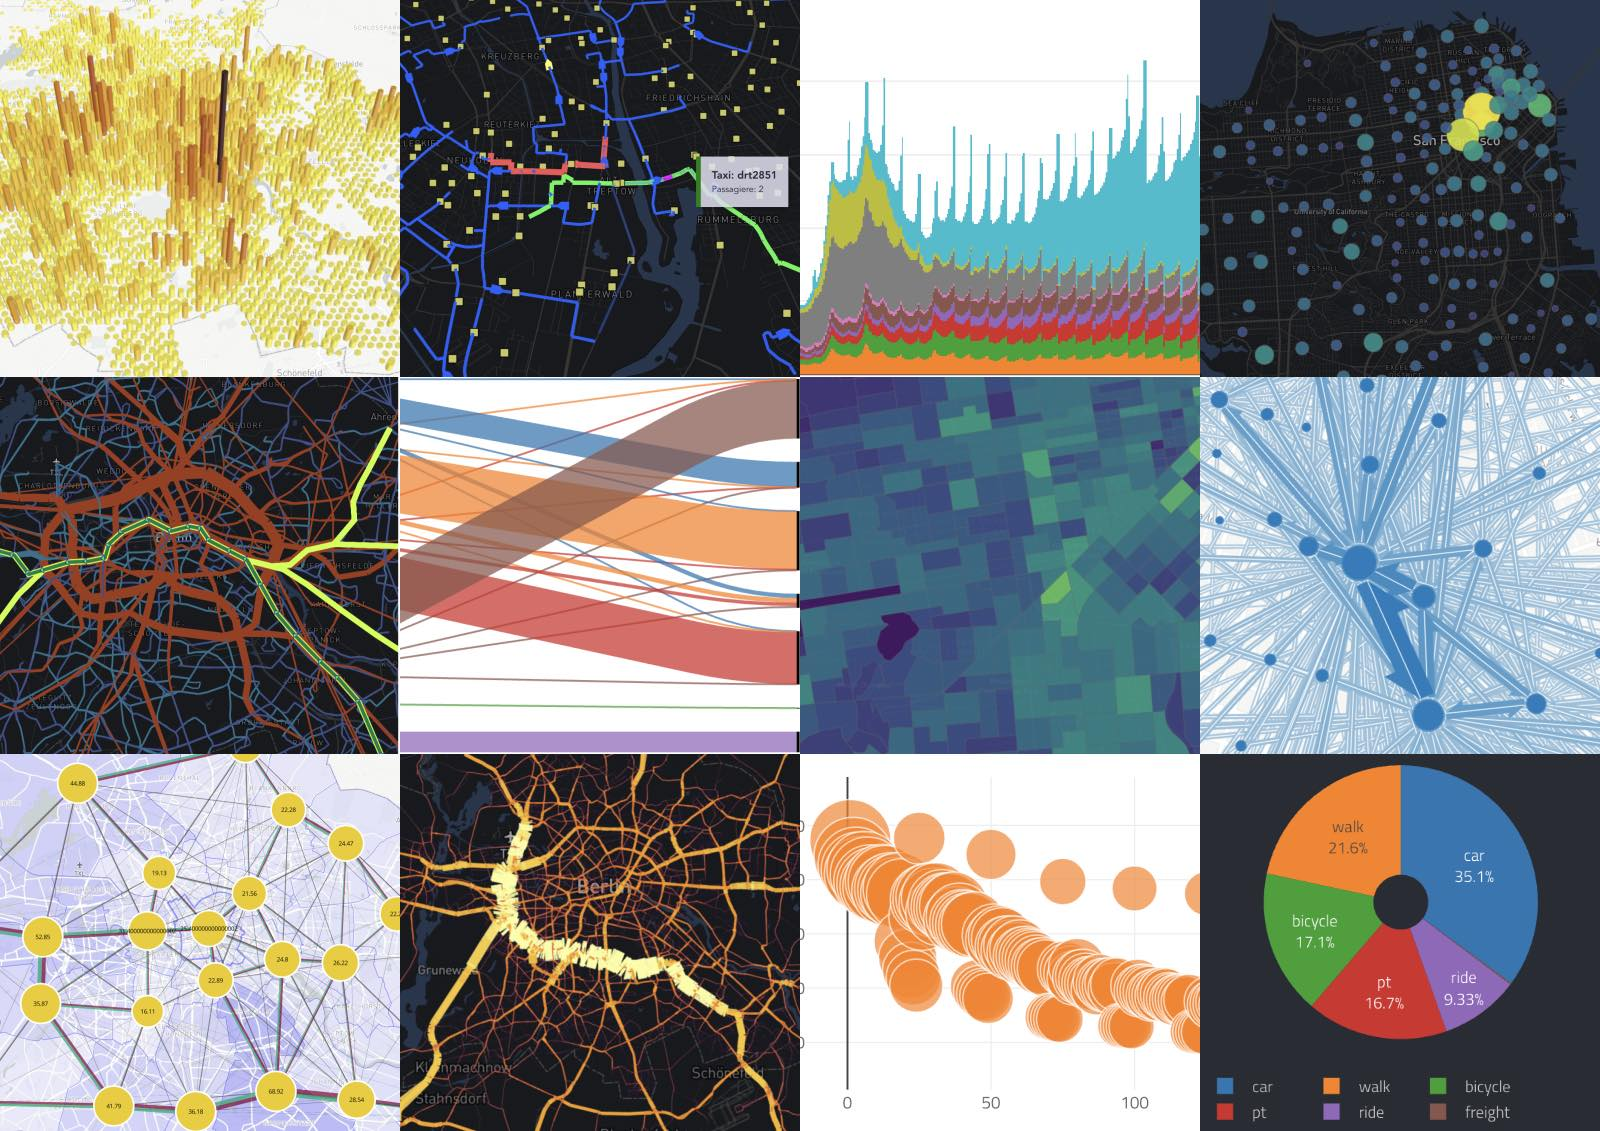
\includegraphics[width=\textwidth]{assets/simwrapper-scrnshot-collage.jpg}
\end{figure}

SimWrapper has extensive user documention online at \url{simwrapper.github.io}. This appendix provides a snapshot of the documentation at the time of publication. \emph{Note this is a direct snapshot of the online documentation and is not written in a scientific tone.}

Currently, SimWrapper is at release version 2.3.0 and includes many features for creating generally useful data dashboards, along with MATSim-specific visualization types.

\section{Getting, installing and using SimWrapper}
\textbf{SimWrapper} is a unique, web-based data visualization tool for
researchers building disaggregate transportation simulations with
software such as \href{https://matsim.org}{MATSim} and
\href{https://activitysim.github.io}{ActivitySim}.

SimWrapper creates interactive dashboards and provides many statistical
views and chart types, just like other viz frameworks. But SimWrapper
also knows a lot about transportation, and has good defaults for
producing visualizations of network link volumes, agent movements
through time, aggregate area maps, scenario comparison, and a lot more.

You don't need to code in any language to use SimWrapper -- you point it
at your files, and write some small text (YAML) configuration files to
tell SimWrapper what to do. SimWrapper does the rest!

If you know JavaScript, the open-source code and plugin architecture of
SimWrapper allows you to fork the project and create your own
visualizations, too. But you don't need to know JavaScript if SimWrapper
already does what you need.

\hypertarget{how-simwrapper-works}{%
\subsection{How SimWrapper works}\label{how-simwrapper-works}}

SimWrapper is a web platform that can display either individual
full-page data visualizations, or collections of visualizations in
``dashboard'' format. It expects your simulation outputs to just be
regular files on your filesystem somewhere; there is no centralized
database or cloud server that you need to upload your results to.

To tell SimWrapper where your data files are:

\begin{itemize}
\tightlist
\item
  You can view files on your local computer directly in Google Chrome
  and Edge, or by running a tiny file server locally for Safari and
  Firefox (Chrome is recommended)
\item
  At VSP TU-Berlin, we have connected SimWrapper to our public file
  server, and use that for producing publicly accessible data dashboards
\item
  You can set up your own local SimWrapper server on your LAN or use
  internet file storage
\item
  If you have access to a remote compute cluster, you can see those
  files too if you mount the remote file system on your machine.
\end{itemize}

Once you point SimWrapper to your collection of files, some
visualizations will be immediately available --- depending on what
SimWrapper finds in your folder.

For other visualizations, you'll create tiny configuration files (in
YAML format) which tell SimWrapper what to load, how to lay out the
dashboards, and which provide all the config details to get it started.
These files can be collected in project folders and then will apply to
all runs in a set of folders, if you want.

\hypertarget{getting-started-with-simwrapper}{%
\subsection{Getting Started with
SimWrapper}\label{getting-started-with-simwrapper}}

\hypertarget{simwrapper-online-demo}{%
\subsubsection{1. SimWrapper online demo}\label{simwrapper-online-demo}}

Go to \url{https://vsp.berlin/simwrapper} and explore the project
dashboards on the home page there. You'll get an idea of what's possible
with SimWrapper.

\hypertarget{copying-the-demo-files-and-exploring-them-locally}{%
\subsubsection{2. Copying the demo files and exploring them
locally}\label{copying-the-demo-files-and-exploring-them-locally}}

We've created a SimWrapper example project with sample datasets and
configurations ready to go.

\begin{itemize}
  \tightlist
  \item
    Download and unzip the latest
\href{https://github.com/simwrapper/simwrapper-example-project/archive/refs/heads/main.zip}{simwrapper-example-project.zip}
from the GitHub
\href{https://github.com/simwrapper/simwrapper-example-project}{example
project}
  \item Open Google Chrome (for this demo, it's easiest to use Chrome
because it has an API for accessing local files on your computer;
Firefox and Safari don't)
  \item Click \textbf{Add Local folder\ldots{}} and
navigate to the unzipped folder you just created. You'll see lots of
example visualizations and dashboards!
  \item You can open any of datasets or
the \texttt{.yaml} configuration files in the archive to see how the
files and parameters are specified. Change things and see what happens.
\end{itemize}

\hypertarget{going-further}{%
\subsubsection{3. Going further}\label{going-further}}

The guides to the left cover the basics of getting up and running,
building your first visualizations and dashboards, and publishing
results online.

There is also an API Reference page for each type of visualization,
where you can find all of the configuration details for each type.

Finally, our
\href{https://github.com/simwrapper/simwrapper/issues}{GitHub Issue
Tracker} is the best place to ask questions and seek help.


\begin{center}\rule{0.5\linewidth}{0.5pt}\end{center}
\section{File management}
\textbf{SimWrapper} doesn't have a back-end database; it reads the files
in folders that you give it access to.

Depending on where your files are, this may require some configuration!

\begin{itemize}
\tightlist
\item
  At TU Berlin, everything in our public subversion server is already
  accessible. Check it out here:
  \href{https://vsp.berlin/simwrapper}{vsp.berlin/simwrapper}
\item
  You can view files on your local computer, see below
\item
  If you have SSH access to network compute-cluster servers, you can
  mount the remote filesystems and they behave as if they are local; see
  below
\item
  You can also set up remote file storage on cloud servers such as
  Amazon etc.
\end{itemize}

\hypertarget{local-folders-on-your-computer}{%
\subsection{Local folders on your
computer}\label{local-folders-on-your-computer}}

\textbf{Easy version:} Use Google Chrome or Microsoft Edge to access
files on your local machine. These two browsers have a built-in file
access API which lets you grant access to a folder for viewing, and then
everything just works. From the SimWrapper home page, click
\texttt{Add\ Local\ folder...} to get started.

\noindent\textbf{Hard version:} Other browsers (Safari, Firefox, others) block
local file access by default. The only way to access local files is by
running a small local HTTP server on ``localhost:8000''. This works for
all browsers but Safari has additional measures which make it the worst
choice for this.

For these reasons, we strongly recommend using Google Chrome (or Edge if
that's your thing)

We formerly supported both Python and Java versions of this HTTP server,
but now only the Python 3.x version is supported.

\textbf{Python:} this should work with Python 3.6+:

\begin{enumerate}
\def\labelenumi{\arabic{enumi}.}
\tightlist
\item
  Run \texttt{pip3\ install\ simwrapper} to install the simwrapper
  command-line tool. If you don't have \texttt{pip} installed, you'll
  need to get that set up in your Python environment first.
\item
  \texttt{cd} to the folder you wish to serve, and then run the command
\item
  \texttt{simwrapper\ serve}
\item
  Test that it's working by browsing to \url{http://localhost:8000}. If
  you see a file listing, then it is working
\item
  You can now go to the SimWrapper website and choose ``Local files'' to
  browse your folders inside of SimWrapper!
\item
  You can run multiple copies of the SimWrapper Python tool in separate
  root folders if you wish. Each one will run on the next port, so
  localhost:8001, localhost:8002, etc.
\end{enumerate}

\hypertarget{mounting-remote-file-systems-cluster-compute-services-etc}{%
\subsection{Mounting remote file systems -- cluster compute services
etc}\label{mounting-remote-file-systems-cluster-compute-services-etc}}

You can ``virtually'' mount remote filesystems using the tool
\texttt{sshfs}. It creates an ssh tunnel to the remote machine using
your username/login credentials, and mounts the files it finds there
under a subfolder on your machine.

Once the sshfs tunnel is established, you can browse the files there as
if the files are local on your machine, as above.

\begin{itemize}
\tightlist
\item
  Linux: install \texttt{sshfs} and follow your OS instructions for how
  to mount remote filesystems
\item
  Mac: Use \href{https://osxfuse.github.io/}{MacFUSE} to set up sshfs
\item
  Windows: \href{https://winfsp.dev/}{WinFSP} may provide this; please
  let me know if this works for you
\end{itemize}

\hypertarget{internetcloud-storage}{%
\subsection{Internet/cloud storage}\label{internetcloud-storage}}

SimWrapper can be configured to use any Internet storage that can serve
up file and folder listings similar to Apache or NGINX. Currently, this
means public storage only; no authenticated storage. \emph{{[}to be
enhanced in the future!{]}}

\begin{itemize}
\item
  To set up SimWrapper for internet storage, you need to fork SimWrapper
  and set up your own instance, then define your storage endpoint in the
  file \texttt{src/fileSystemConfig.js} following the examples there.
\item
  If you do not yet have your own instance of SimWrapper set up, follow
  the \href{dev-developing-simwrapper.md}{instructions here}.
\end{itemize}

\textbf{Amazon AWS} You can set up access to Amazon EC2/EFS file storage
by following this guide:
\url{https://docs.aws.amazon.com/efs/latest/ug/wt2-apache-web-server.html}




\begin{center}\rule{0.5\linewidth}{0.5pt}\end{center}
\section{Guide: Getting Started}
Welcome to SimWrapper! Let's get you up and running with the basics.

\begin{itemize}
\tightlist
\item
  This guide uses sample data that's hopefully a lot like the data you
  would have for your projects
\item
  Use Google Chrome or MS Edge for the guide. Other browsers (Firefox,
  Safari) require a \href{file-management}{separate local HTTP server}
  to access local files; for now that's just a stumbling block to
  getting started.
\end{itemize}

\hypertarget{how-it-works-simwrapper-and-file-based-configuration}{%
\subsection{How it works: SimWrapper and file-based
configuration}\label{how-it-works-simwrapper-and-file-based-configuration}}

Most MATSim/ActivitySim outputs such as the \texttt{*.xml.gz} files are
too large to open in a web browser, so SimWrapper provides a set of
\emph{visualization plugins} which can display something useful for you.
Plugins exist for lots of things and the list is growing: link volumes,
agent animations, aggregate area summaries, and more.

Here's how it works: For every visualization you want to create, you
write a small \emph{configuration file} and store it in the same folder
as the inputs for that visualization. We use the YAML text format, which
is a common configuration file format. For each properly named YAML
file, one visualization thumbnail will appear in that folder when you
navigate to the folder in SimWrapper. Clicking on the thumbnail will
open that visualization full-screen.

Generally, a viz will require a specific set of inputs, and those inputs
are usually the result of some \emph{post-processing} of the raw
simulation outputs. It's up to you to do that post-processing and store
the files in the same folder as your config file.

Let's get started with some sample data.

\hypertarget{get-the-sample-data-and-open-it-in-simwrapper}{%
\subsection{1. Get the sample data and open it in
SimWrapper}\label{get-the-sample-data-and-open-it-in-simwrapper}}

\begin{itemize}
\tightlist
\item
  Download
  \href{https://github.com/simwrapper/simwrapper-example-project/archive/refs/heads/main.zip}{simwrapper-example-project.zip}
  from GitHub
\item
  Unzip the file somewhere you can find it easily - Desktop, home
  folder, etc.
\item
  Go to \href{https://simwrapper.github.io/site}{simwrapper.github.io}
  and click \texttt{Add\ folder...} and browse to the folder you just
  created. Grant access to the folder so the SimWrapper site can see the
  files.
  \begin{itemize}
  \tightlist
  \item
    If you are using Firefox, \texttt{cd} to the data folder and run
    \texttt{simwrapper\ here} to start the local HTTP server
  \end{itemize}
\end{itemize}

\hypertarget{explore-the-samples}{%
\subsection{2. Explore the samples}\label{explore-the-samples}}

Each of the subfolders in the example project shows different map views
and capabilities of SimWrapper -- network link plots, statistical
charts, area maps (shapefiles), dashboards, and so on.

\begin{itemize}
\tightlist
\item
  Experiment with the various knobs and configuration settings to see
  how the visualizations can be manipulated
\item
  From your PC file browser, open up the \texttt{viz-*.yaml} files in
  each subfolder to see how each of the visualizations is defined in a
  readable text format.
\item
  Every visualization type has a different filename ``prefix'' to help
  you find them: e.g, \texttt{viz-map-*.yaml} are for shapefiles,
  \texttt{viz-link-*.yaml} are for MATSim network plots, and so on.
\item
  You can edit these YAML files, save, and click Reload on your browser
  to see how your changes affect the visualizations.
\end{itemize}

\hypertarget{create-a-dashboard-with-some-charts}{%
\subsection{3. Create a dashboard with some
charts}\label{create-a-dashboard-with-some-charts}}

The dashboards subfolder shows how you can combine multiple
visualizations into cohesive dashboards.

\begin{itemize}
\tightlist
\item
  The \texttt{dashboard-*.yaml} files define each individual tab in a
  dashboard. It's often nice to name them \texttt{dashboard-1-*.yaml},
  \texttt{dashboard-2-*.yaml} etc, to set them in the order that you
  like.
\item
  Dashboards are laid out in rows: Each row can have multiple panels.
  See the YAML files for how this works!
\end{itemize}

\hypertarget{configuring-dashboard-templates-for-multiple-run-folders}{%
\subsection{4. Configuring dashboard templates for multiple run
folders}\label{configuring-dashboard-templates-for-multiple-run-folders}}

In SimWrapper, everything is folder-based. So \texttt{viz-*.yaml} and
\texttt{dashboard-*.yaml} files in a folder will automatically be
detected and loaded based on their filenames.

If you want to define dashboards that will be used for \textbf{multiple
folders}, such as several runs for a particular project:

\begin{itemize}
\tightlist
\item
  \textbf{Create a folder} named \texttt{simwrapper} in the parent
  project directory.
\item
  Move all dashboard, viz, and template YAMLs into that folder
\item
  Tweak any file paths as necessary, so that relative file names resolve
  properly.
\item
  The base folder for a dashboard is the \emph{folder you are viewing},
  not the dashboard template folder.
\item
  You can have multiple \texttt{simwrapper} folders all the way up your
  folder hierarchy; dashboard panels will be generated based on
  filename, and each found dashboard will be displayed as a tab on the
  folder view.
\end{itemize}

\hypertarget{more-details-on-visualizations-and-their-yaml-files}{%
\subsection{5. More details on visualizations and their YAML
files}\label{more-details-on-visualizations-and-their-yaml-files}}

Here is an example YAML config file for a link-volume summary:

\textbf{viz-links-example.yaml:}

\begin{lstlisting}[]
  title: 'Taxi Passengers'
  description: 'Hourly passenger pickups'
  csvFile: 'vol_passengers.csv'
  geojsonFile: '../road-network.json.gz'
  projection: 'EPSG:25832'
  sampleRate: 0.10
\end{lstlisting}

This config names two files, a CSV of link volumes and a zipped JSON
file of the MATSim road network, and some parameters needed for the viz
to work. Those files are outputs of some post-processing scripts
described in the plugin docs.

If you wanted to look at several different link volume plots from the
same model run, (e.g.~for vehicle counts instead of passengers), you
would make a copy of this file, give it a different name, and edit the
\texttt{csvFile} parameter to point to the correct CSV.

This is a very different paradigm than most ``point and click'' GIS
tools, but we have found that the ability to script and cut/paste the
config files has been a huge time saver and also reduces manual errors.

\begin{quote}
\emph{Make sure that your files are allowed to be ``world-readable'' before
you publish anything to public-svn! Once files are pushed to public-svn,
they are not secured in any way; anyone on the internet can access them!}
\end{quote}


\begin{center}\rule{0.5\linewidth}{0.5pt}\end{center}
\section{Guide: Dashboards in Depth}
A dashboard is a page laid out with multiple charts, plots, and
visualizations all together. You define the layout with a YAML
configuration file which contains the types of plots and their
configurations all in one place.

\begin{figure}[H]
  \centering
  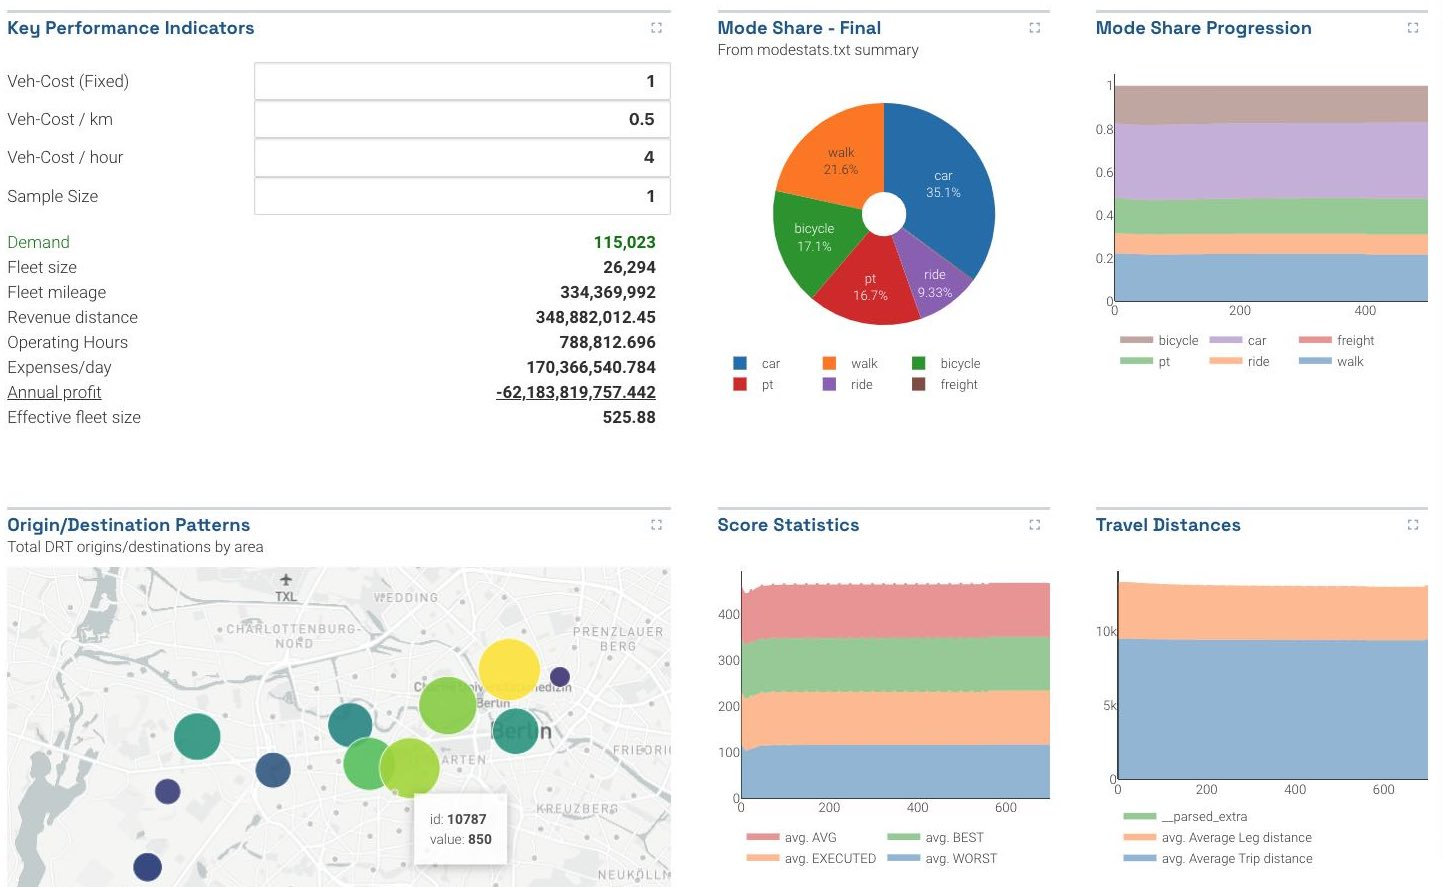
\includegraphics[width=0.8\textwidth]{assets/dashboard.jpg}
  \caption{Dashboards usually show several at-a-glance summary metrics.}
\end{figure}

A folder containing any number of \texttt{dashboard-*} YAML files show
the dashboard instead of the usual folder browser view. When multiple
dashboard YAML files exist, they will be shown as multiple navigation
tabs on the page.

\hypertarget{defining-a-dashboard}{%
\subsection{Defining a dashboard}\label{defining-a-dashboard}}

Start with the example below and edit as necessary. YAML is
\emph{extremely picky} about white space and indentation, like Python.
Be careful!

\hypertarget{header}{%
\subsubsection{Header}\label{header}}

A dashboard requires a top-level \texttt{header} containing \emph{tab}
and \emph{title} and optional \emph{description.}

\begin{lstlisting}
  header:
  tab: 'Summary'
  title: 'Top-Level Summary Statistics'
  description: 'At-a-glance figures we usually look at' #optional
\end{lstlisting}

\hypertarget{layout}{%
\subsubsection{Layout}\label{layout}}

Below the header, a dashboard also requires a \texttt{layout} section
which defines a set of named \textbf{rows}. The row name themselves are
not displayed anywhere; they are just there to help you organize the
file.

\noindent\textbf{row}: Each \texttt{row} can contain either (1) the properties of
a full-width panel, or (2) a YAML \textbf{list} of properties for panels
that will be laid out horizontally in the row. YAML lists have a strange
syntax with \texttt{-} hyphens marking the beginning of a list item.
It's best to just look at the example below.

By default, multiple panels are laid out from left to right, in equal widths. (But see \emph{width} option further below)

\begin{lstlisting}
  layout:
    myRow1: # this row has one full-width chart
      type: bar
      title: 'My Bar Chart'
      dataset: mycsvdata.csv
      # ...

    # next row has two charts, using the '-' YAML list syntax
    myMultiRow:
      - type: bar
        title: 'My Bar Chart'
        dataset: mycsvdata.csv
        # ...

      - type: table
        title: 'My Summary Table'
        config: summary-table.yaml
\end{lstlisting}

That indentation in the example above is extremely important!
Indentation is how YAML interprets the grouping of elements.

\noindent\textbf{Chart/plot details:} Each element in a row has the following
properties. This defines the actual chart that will be displayed.

\begin{itemize}
\tightlist
\item
  \textbf{type} Required: the chart or plot type, e.g.~\texttt{pie},
  \texttt{bar}, \texttt{flowmap}, etc. See the individual chart docs for
  all available plots.
\item
  \textbf{title} The name of the plot
\item
  \textbf{description} A brief description (optional)
\item
  \textbf{height} You can set \emph{relative height} by adding the
  \texttt{height:} parameter (default: 5)
\item
  \textbf{width} You can set \emph{relative widths} by adding the
  \texttt{width:\ {[}number{]}} property. Panels have a default width of
  1. Thus in a row with 3 charts, if the width of the first object is 2,
  then {[}2+1+1{]} means the first object fills 50\% of the row, and the
  remaining two objects fill 25\% each. (default: 1)
\item
  \textbf{Other properties} Every viz type has its own set of
  properties. Include those as separate \texttt{key:\ value} lines in
  the configuration, as needed. See the individual chart docs in the API
  Reference; \emph{The chart type determines the set of valid
  properties!}
\end{itemize}

\hypertarget{example-dashboard-summary.yaml}{%
\subsection{Example:
dashboard-summary.yaml}\label{example-dashboard-summary.yaml}}

Here is a full example dashboard, pulling all of the above together.
Note especially the indentation and the use of \texttt{-} to denote YAML
lists.

\begin{lstlisting}
header:
  tab: Summary
  title: My Summary Dashboard
  description: 'Examples of various chart types'

layout:
  row1: # this row has two charts
    - title: 'Mode Share - Final'
      description: 'From modestats.txt summary'
      type: 'pie'
      width: 1
      dataset: '*modestats.txt'
      useLastRow: true
      ignoreColumns: ['Iteration']

    - title: 'Example Bar Plot'
      description: 'Distance over Iteration'
      type: 'bar'
      width: 2
      usedCol: [distance_m_mean, directDistance_m_mean]
      legendName: [Distance (mean), Direct Distance (mean)]
      skipFirstRow: true
      dataset: '*drt_customer_stats_drt_short.csv'
      x: 'iteration'
      yAxisName: 'Distanz'
      xAxisName: 'Iteration'

  secondRow: # this row has just one plot
    title: 'Example Line Plot'
    description: 'Distance over Iteration'
    type: 'line'
    width: 1
    usedCol: [distance_m_mean, directDistance_m_mean]
    legendName: [Distance (mean), Direct Distance (mean)]
    skipFirstRow: false
    dataset: '*drt_customer_stats_drt.csv'
    x: 'iteration'
    yAxisName: 'Distance'
    xAxisName: 'Iteration'
\end{lstlisting}

\begin{center}\rule{0.5\linewidth}{0.5pt}\end{center}
\section{Guide: Building Project Sites}
You can hide all of the SimWrapper ``chrome'' such as the folder
browser, and provide custom header/footer for each page using CSS. This
is useful for building special-purpose tools that might be
outward-facing, for example.

\hypertarget{setting-up-a-project-site}{%
\subsection{Setting up a project site}\label{setting-up-a-project-site}}

\begin{itemize}
\tightlist
\item
  Create \texttt{simwrapper-config.yaml} in your project folder
\item
  Define the custom footer and header in markdown files
\item
  Use css in a custom CSS file to present as you wish
\end{itemize}

There are two general configuration options:

\textbf{hideLeftBar:} True/false, hides the left-side folder browser
panel

\textbf{fullWidth:} True/false, true removes the fixed-width centered
panel if you want a full-screen experience

\hypertarget{sample-simwrapper-config.yaml-file}{%
\paragraph{Sample simwrapper-config.yaml
file}\label{sample-simwrapper-config.yaml-file}}

\begin{lstlisting}
  hideLeftBar: true
  fullWidth: true
  header: header.md
  footer_en: footer.md
  footer_de: footer.md
  css: custom.css
\end{lstlisting}

\paragraph{Sample header.md}
Sample header.

\begin{lstlisting}
  !-- header image logo -->
  <img class="project-logo"
       src="https://svn.vsp.tu-berlin.de/repos/public-svn/matsim/scenarios/countries/de/kelheim/projects/KelRide/logos/KelRide-text.png"
  />
\end{lstlisting}

\paragraph{Sample footer.md}
Sample footer.

\begin{lstlisting}
  <footer>
  <div class="container">
    <div class="logos">
        <img src="https://svn.vsp.tu-berlin.de/repos/public-svn/matsim/scenarios/countries/de/kelheim/projects/KelRide/logos/KelRide-text.png"/>
        <img src="https://svn.vsp.tu-berlin.de/repos/public-svn/matsim/scenarios/countries/de/kelheim/projects/KelRide/logos/LK_Kelheim.png"/>
        <img src="https://svn.vsp.tu-berlin.de/repos/public-svn/matsim/scenarios/countries//de/duesseldorf/projects/komodnext/website/logos/TU.svg"/>
    </div>

    <div class="menu">
      VSP / TU Berlin
      (c) 2023 TU Berlin. <a href="https://vsp.berlin/impressum">Impressum</a>
    </div>
  </div>
  </footer>

\end{lstlisting}

\paragraph{Sample custom.css}

Custom CSS can be quite extensive, refer to the online documentation for examples.




\begin{center}\rule{0.5\linewidth}{0.5pt}\end{center}
\section{Reference: MATSim Network link plots}
\begin{figure}[H]
  \centering
  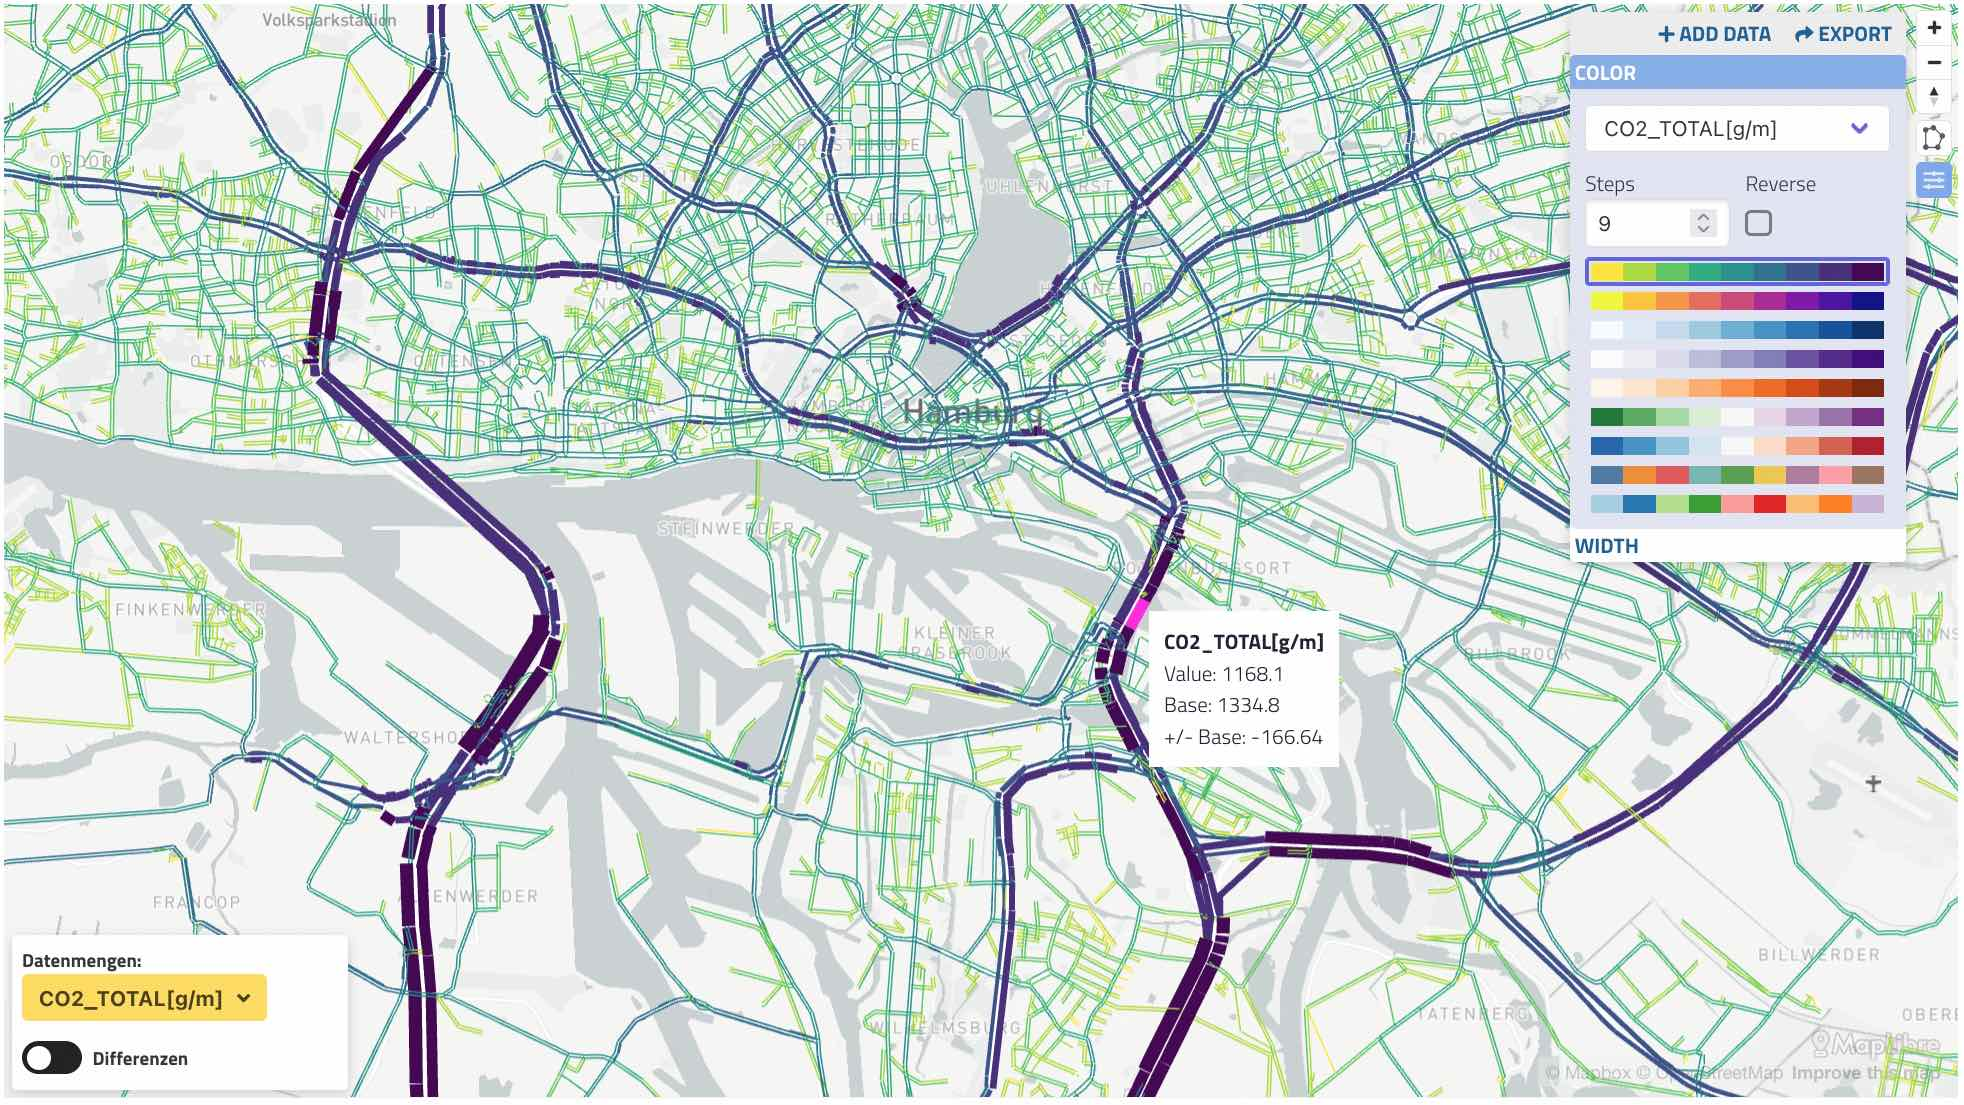
\includegraphics[width=0.8\textwidth]{assets/links.jpg}
  \caption{Bandwidth plot. Colors and widths can specify different data,}
\end{figure}

The network link plot supports typical transport ``bandwidth plots'' as
well as many other types of data. If your data can be attached to link
via the link ID, you can use this plot!

Supports display of data from multiple datasets, including ``difference
plots'' which can compare two datasets, e.g.~base vs.~build.

\hypertarget{usage}{%
\subsection{Usage}}

You can create a link visualization as a standalone view, as part of a
dashboard, or you can create it interactively from a raw network file.

\begin{enumerate}
\def\labelenumi{\arabic{enumi}.}
\item
  A standalone visualization is defined with a file named
  \texttt{viz-links-*.yaml} in your working folder. Each yaml file
  matching that pattern will produce a separate link volume diagram.
\item
  Link plots can be included in \url{dashboards} using
  \texttt{type:\ links}. See the example YAML config below.
\item
  Or, you can open a network file directly by browsing to it from the
  SimWrapper site, and then click \textbf{Add Data} in the configuration
  panel in the upper right to attache CSV data files to it. Once you
  have added data and configured the colors and widths, use the
  \textbf{Export} button to download the YAML file. Your browser will
  probably place the file in your Downloads folder; you'll need to move
  it to your data folder name it appropriately.
\end{enumerate}

\textbf{Standalone: viz-links-example.yaml}

\begin{lstlisting}
  title: 'Passagiers in DRT Vehicles'
  description: 'Hourly passengers, build scenario'
  csvFile: 'hourlyTrafficVolume-drt-vehicles.csv'
  csvBase: '../base/hourlyTrafficVolume-drt-vehicles.csv'
  network: '*output_network.xml.gz'
  thumbnail: thumbnail-roads.jpg
\end{lstlisting}

\begin{lstlisting}
  header:
  title: My Dashboard

layout:
  row1:
    - title: 'Link example'
      description: 'Sample data'
      type: links
      height: 8
      props:
        network: '../input/baseCase/hamburg-v2.0-network-with-pt-hvvArea.geo.json.gz'
        projection: EPSG:25832
        center: 13.4684, 56.6787
        zoom: 9
        showDifferences: true
        datasets:
          csvFile: 'output/reallab2030/accidentCosts.csv.gz'
          csvBase: '../base/output/accidentCosts.csv.gz'
        display:
          color:
            dataset: csvFile
            columnName: 18:00-20:00_Costs[EUR]
            colorRamp:
              ramp: Viridis
              steps: 9
          width:
            dataset: csvFile
            columnName: CostsperYear[EUR]
            scaleFactor: 100
\end{lstlisting}
\textbf{Dashboard: dashboard-example.yaml}

\hypertarget{attaching-csv-data-to-your-network-link-visualization}{%
\subsection{Attaching CSV data to your network link
visualization}\label{attaching-csv-data-to-your-network-link-visualization}}

Any CSV datafile can be used to attach data to the network
visualization. Each link in your network must have a unique ID, and the
CSV file must have one row per link, with the link ID as the first
column. No other arrangement will work.

Use whatever method you like to produce a CSV for your data; most of us
either build the dataset from event listeners within MATSim, or through
post-processing using Python or R. But as long as you can create a CSV
file with link IDs and values that you need, the method doesn't matter.

\textbf{Column names} The CSV file should have a header line as the
first line of the file. This header should contain column names, or
labels, for every column. E.g. hour of the day, type of pollutant, etc.

\begin{itemize}
\tightlist
\item
  First column \textbf{must be} the link ID, identical to the link IDs
  in the network file
\item
  All remaining columns will be available and will be labeled according
  to the file header.
\item
  \textbf{Note:} older versions of SimWrapper used to autogenerate a
  ``sum'' column. This has been removed. If you want to show a ``sum''
  total column, you will have to calculate it yourself as a separate
  column in your data file.
\end{itemize}

\begin{center}\rule{0.5\linewidth}{0.5pt}\end{center}

\hypertarget{yaml-fields-explained}{%
\subsection{YAML fields explained}}

*Filename fields** can refer to subfolders and to parent folders using
\texttt{"../"}.

\begin{itemize}
\tightlist
\item
  example: \texttt{network:\ :\ "../networks/base.json.gz"}
\end{itemize}

This works as far up the hierarchy as the base of the filesystem,
specified in \texttt{fileConfig.js} but no further.

\hypertarget{field-descriptions}{%
\subsubsection{Field descriptions}\label{field-descriptions}}

\textbf{title:} (optional) title of the visualization, appears right on
top of the map. If a title is specified both under \texttt{general} and
under \texttt{props}, the one under \texttt{general} will be used.

\noindent\textbf{description:} (optional) description of the visualization,
appears between title and map. If a description is specified both under
\texttt{general} and under \texttt{props}, the one under
\texttt{general} will be used.

\noindent\textbf{csvFile:} dataset in CSV or TSV format.

\begin{itemize}
\tightlist
\item
  Columns are autodetected and will split at commas, semicolons, or
  tabs.
\item
  Numbers \textbf{must be in 1234.56 format} -- European
  ``1.234.567,00'' formats will not work.
\end{itemize}

\noindent\textbf{csvBase:} (optional) ``base'' dataset for difference plots. If
\texttt{csvBase} is specified, ``diff mode'' will be enabled and
difference plots can be automatically generated.

\begin{itemize}
\tightlist
\item
  Differences are always calculated as
  \texttt{\textquotesingle{}csvFile\ -\ csvBase\textquotesingle{}}
\end{itemize}

\noindent\textbf{network:} Specify either at MATSim
\texttt{output\_network.xml.gz} network file, or a geojson-format
network file. The geojson format loads much faster, but requires that
you create it first.

\begin{itemize}
\tightlist
\item
  Use the python script
  \href{https://raw.githubusercontent.com/simwrapper/simwrapper/master/scripts/create-geojson-network.py}{create-geojson-network.py}
  to create a geojson network from a MATSim network.xml.gz file.
\item
  Command is
  \texttt{python\ create-geojson-network.py\ {[}my\_output\_network.xml.gz{]}\ {[}Projection{]}}
\item
  and will create a file with the name \texttt{mynetwork.geo.json.gz}.
\end{itemize}

\noindent\textbf{projection:} projection must be given! Format
\texttt{EPSG:25832} etc.

\noindent\textbf{geojsonFile:} (deprecated) - same as \texttt{network}.

\noindent\textbf{thumbnail:} (optional) file path to a thumbnail in jpg format

\noindent\textbf{center:} (optional) coordinates that the map centers on. Can be
provided as array or string. If it is not provided, a center is
calculated using a sampling of the data.

\noindent\textbf{zoom:} (optional) zoom level of the map. If it is not provided,
the zoom level 9 is used.

\noindent\textbf{showDifference:} allows difference plots to be created if a base
case is provided. Should be \texttt{true}.

\noindent\textbf{display:} The optional display section includes details of the
color and width data specifications.

\hypertarget{defining-colors-and-widths}{%
\subsection{Defining Colors and
Widths}\label{defining-colors-and-widths}}

Both colors and widths can be based on the CSV data. They are defined in
the \texttt{display:} section of the YAML; see the example above.

\hypertarget{color}{%
\subsubsection{Color}\label{color}}

The \texttt{color} section may include the following properties:

\begin{itemize}
\tightlist
\item
  \textbf{dataset} required. The ID of the csv datafile itself; in the
  example above, \texttt{csvFile} is one key and \texttt{csvBase} is
  another. This tells SimWrapper which dataset you want to use.
\item
  \textbf{columnName} The name of the column containing color values
\item
  \textbf{colorRamp} This section can have multiple settings:

  \begin{itemize}
  \tightlist
  \item
    \texttt{ramp}: The name of the color progression; can be
    \texttt{Viridis}, \texttt{Plasma}, \texttt{Blues}, \texttt{Purples},
    \texttt{Oranges}, \texttt{PRGn}, \texttt{RdBu}, \texttt{Tableau10},
    \texttt{Paired}. Note that \texttt{PRGn} and \texttt{RdBu} are
    \textbf{diverging scales}, while \texttt{Tableau10} and
    \texttt{Paired} are appropriate for \textbf{categorical} instead of
    sequential data.
  \item
    \texttt{reversed} true or false, flips the order of colors
  \item
    \texttt{steps} the number of different colors in the progression;
    default is 9.
  \end{itemize}
\end{itemize}

\hypertarget{width}{%
\subsubsection{Width}\label{width}}

The \texttt{width} section includes the following properties:

\begin{itemize}
\tightlist
\item
  \textbf{dataset} required. The ID of the csv datafile itself; in the
  example above, \texttt{csvFile} is one key and \texttt{csvBase} is
  another. This tells SimWrapper which dataset you want to use.
\item
  \textbf{columnName} The name of the column containing width values
\item
  \textbf{scaleFactor} Values will be \textbf{divided by} this scaling
  factor. Set this to \texttt{0} to have constant, paper-thin widths.
\end{itemize}

\paragraph{example-data.csv} Sample CSV data

\begin{verbatim}
link;01:00:00;02:00:00;03:00:00;04:00:00;05:00:00;06:00:00;00;00
72539930;0;0;0;0;7;13;20;16;13;15;18;17;32;25;29;55;53;43;48;12;12;
42868713;0;0;0;0;0;0;0;0;0;0;0;0;0;1;0;0;1;1;0;0;0;0;0;0;0;0;0;0;0
72539936;0;1;0;0;17;57;63;52;51;47;49;59;78;67;73;113;99;98;107;47;
6173553;0;1;0;3;5;1;10;10;9;3;8;4;6;3;4;9;5;7;4;2;1;1;1;2;0;1;0;0;0
\end{verbatim}

\hypertarget{deprecated-fields-do-not-use}{%
\subsection{Deprecated fields, do not
use:}\label{deprecated-fields-do-not-use}}

\textbf{shpFile,dbfFile, shpFileIdProperty:} (deprecated) filenames for
the alternative, slower network file in shapefile format. Don't use this
if you have created the geojson network file above.

\noindent\textbf{widthFactor:} (deprecated) Width values used to be uniformly
scaled by this value.

\noindent\textbf{sampleRate:} (deprecated) This option used to specify the MATSim
simulation sample rate; i.e.~a 1\% sample would use \texttt{0.01} here
so that volumes were scaled properly. This is NOW IGNORED; you must
scale your CSV data appropriately.


\begin{center}\rule{0.5\linewidth}{0.5pt}\end{center}
\section{Reference: MATSim Carrier/Freight viewer}
\begin{figure}[H]
  \centering
  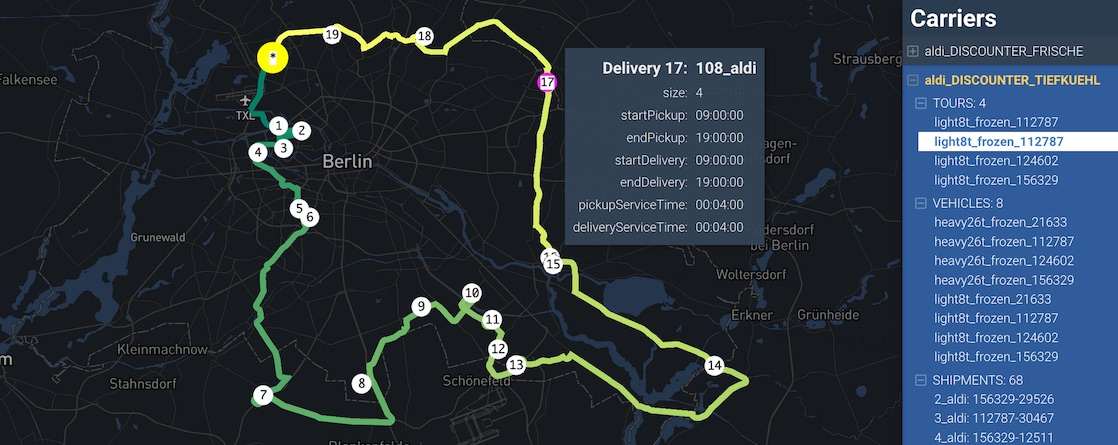
\includegraphics[width=0.8\textwidth]{assets/carriers.jpg}
  \caption{MATSim carrier plans}
\end{figure}


\hypertarget{usage}{%
\subsection{Usage}}

Either the MATSim carriers output file \texttt{output\_carriers.xml}, or a file named \texttt{viz-carrier*.yaml} must be present in the working folder.

If no YAML file is specified and a filename matching pattern "*output\_carriers.xml.gz" is found, it will be loaded with a network file matching the same file pattern.

\textbf{viz-carrier-example.yml}

\begin{lstlisting}
  title: 'Grocery freight network'
  description: '2020 Project'
  network: output_network.xml.gz
  carriers: output_carriers.xml.gz
  center: [13.391, 52.515]
\end{lstlisting}

\hypertarget{yaml-fields-explained}{%
\subsection{YAML fields explained}}

\noindent\textbf{network:} Network filename. Both \texttt{.json.gz} and \texttt{xml.gz} network
files are supported, but JSON-based files load \emph{much} faster.

\noindent\textbf{carriers:} Name of the output\_carriers xml file

\noindent\textbf{center:} Use this to force the map center point.
\texttt{{[}long,lat{]}}


\begin{center}\rule{0.5\linewidth}{0.5pt}\end{center}
\section{Reference: MATSim DRT/Vehicle Animation Viewer}
\begin{figure}[H]
  \centering
  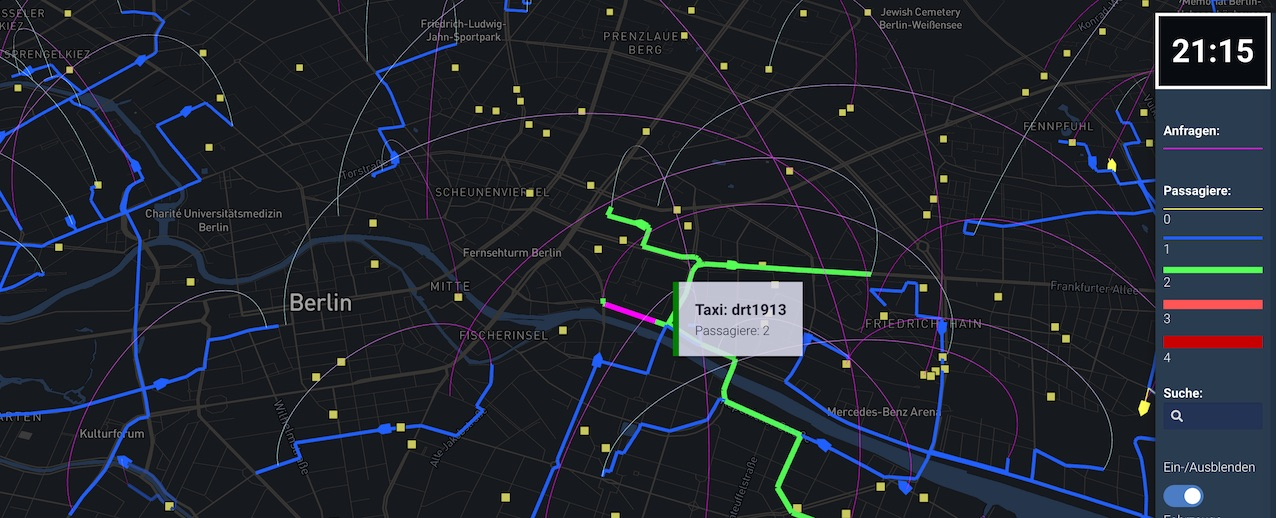
\includegraphics[width=0.8\textwidth]{assets/drt.jpg}
  \caption{Animation of DRT vehicle, paths, and passenger requests}
\end{figure}

\hypertarget{usage}{%
\subsection{Usage}}

A file named \texttt{viz-vehicle-*.yml} must be present in working
folder. Each yml file matching that pattern will produce a separate DRT
visualization.

\textbf{drt-example.yml}

\begin{lstlisting}
  title: 'Dynamic Response Shared Taxis'
  description: Inactive Sammeltaxis (Quadrat); Aktive Sammeltaxis (yellow)
  drtTrips: drt-vehicles.json.gz
  thumbnail: thumbnail-vehicles.jpg
  center: [13.391, 52.515]
\end{lstlisting}

\hypertarget{yaml-fields-explained}{%
\subsection{YAML fields explained}\label{yaml-fields-explained}}

\noindent\textbf{drtTrips:} the output from the
\href{https://github.com/simwrapper/simwrapper/raw/master/scripts/parse-drt-link-events.py}{parse-drt-link-events.py}
script, gzipped for best performance

\noindent\textbf{center:} Use this to force the map center point.
\texttt{{[}long,lat{]}}


\begin{center}\rule{0.5\linewidth}{0.5pt}\end{center}
\section{Reference: MATSim Public Transport Network Viewer}
\begin{figure}[H]
  \centering
  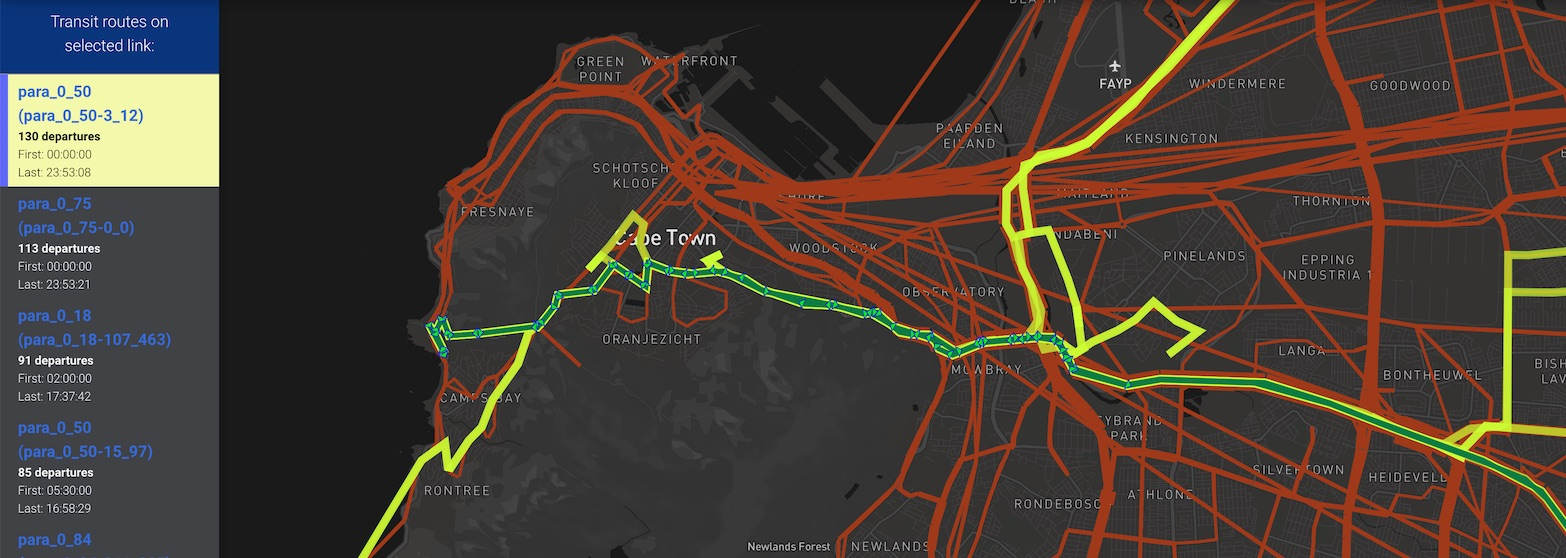
\includegraphics[width=0.8\textwidth]{assets/transit.jpg}
  \caption{Transit routes and ridership}
\end{figure}

This visualization depicts transit routes and lines, and can also display ridership data if available.

\hypertarget{usage}{%
\subsection{Usage}}

No YAML is required. If the run folder contains a
\texttt{*output\_transitSchedule.xml.gz} file, then this view will be
available and the transit route supply can be explored.

If the run folder also contains
\texttt{*pt\_stop2stop\_departures.csv.gz} then the transit ridership
(demand) will also be loaded. This may take a few moments to load.

\hypertarget{exploring-transit}{%
\subsubsection{Exploring transit}\label{exploring-transit}}

Click on any transit link to see the list of transit routes which
traverse that link. You can select any individual route from the details
panel to see the extent of the route.



\begin{center}\rule{0.5\linewidth}{0.5pt}\end{center}
\section{Reference: Aggregate Origin/Destination Flows}
\begin{figure}[H]
  \centering
  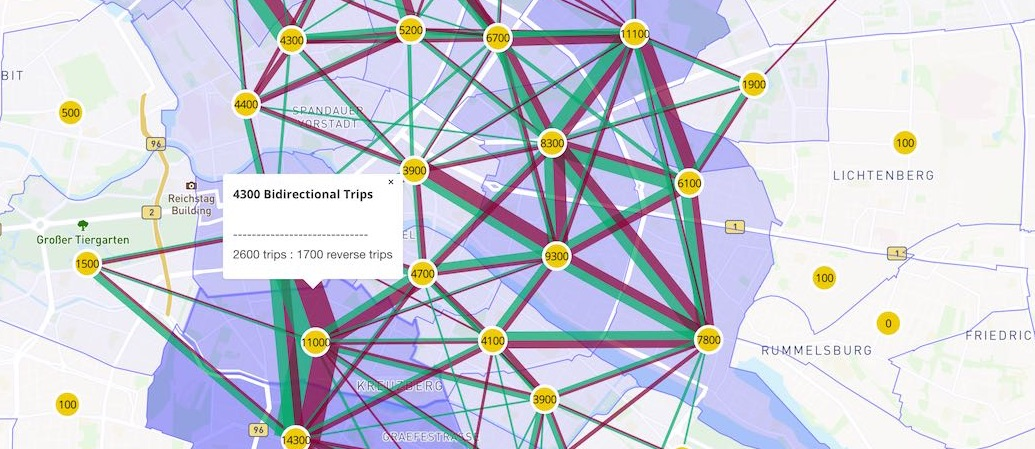
\includegraphics[width=0.8\textwidth]{assets/aggregate-od.jpg}
  \caption{Aggregate Origin/Destination, or ``Spider'' Diagram}
\end{figure}

This visualizion shows aggregated flows between areas defined by a shapefile.
The default view shows everything all at once for every
centroid-to-centroid pair. This can be overwhelming, so you can also
click on an individual centroid to see just the flows to and from that
selected zone.

\hypertarget{usage}{%
\subsection{Usage}}

A file named \texttt{viz-od*.yml} must be present in working folder.
Each yml file matching that pattern will produce a separate Aggregate
O/D diagram.

\textbf{viz-od-example.yml}

\begin{lstlisting}
  # all of the below are required except description and idColumn.
  title: 'My Aggregate Viz'
  description: 'this will be in the sidebar'
  shpFile: Bezirksregionen_zone_GK4_fixed.shp
  dbfFile: Bezirksregionen_zone_GK4_fixed.dbf
  csvFile: od-analysis-hourly-drt.csv
  projection: GK4
  scaleFactor: 100
  idColumn: 'id'
  lineWidth: 50
\end{lstlisting}

\hypertarget{input-files}{%
\subsection{Input Files}}

\textbf{Shapefile:} The DBF data must contain a column with the ID of
the zones/regions. This ID will be used to identify the O/D flows in the
CSV file

\begin{itemize}
\tightlist
\item
  if the \texttt{idColumn} is not specified in YAML then the default
  \texttt{id} will be used.
\item
  If no ID column can be found, then the plot will attempt to use the
  first column in the DBF file.
\end{itemize}

\noindent\textbf{O/D CSV File format:}

\begin{itemize}
\tightlist
\item
  Header line contain labels; first two column names will be used for
  from/to (e.g.~origin/destination)
\item
  Column 1: `From' category
\item
  Column 2: `To' category.
\item
  All further columns list flows from/to. For example, there could be 24
  columns, one for each hour of travel
\end{itemize}

\begin{lstlisting}
origin;destination;1;2;3;4;5;6;7;8;9;10;11;12;13;14;15;16;17
88;88;0;0;0;0;0;0;0;0;0;0;0;0;0;0;0;0;0;0;0;0;0;0;0;0
88;89;0;0;0;0;0;0;0;0;0;0;0;0;0;0;0;0;0;0;0;0;0;0;0;0
88;110;0;0;0;0;0;0;0;0;0;0;0;0;0;0;0;0;0;0;0;0;0;0;0;0
88;111;0;0;0;0;0;0;0;0;0;0;0;0;0;0;0;0;0;0;0;0;0;0;0;0
88;112;0;0;0;0;0;0;0;0;0;0;0;0;0;0;0;0;0;0;0;0;0;0;0;0
etc...
\end{lstlisting}

\hypertarget{configuration-parameters}{%
\subsection{Configuration Parameters}\label{configuration-parameters}}

\noindent\textbf{projection:} Coordinate projection, such as ``EPSG:31468'' or
``GK4''

\noindent\textbf{scaleFactor:} Factor to scale all values -- to handle 1\% or
10\% scenarios, for example

\noindent\textbf{lineWidth:} Starting width scaling of lines

\noindent\textbf{idColumn:} Data column in shapefile which contains the ID for
regions/zones (default ``id'')


\begin{center}\rule{0.5\linewidth}{0.5pt}\end{center}
\section{Reference: Bar, Area, and Line Charts}
\begin{figure}[H]
  \centering
  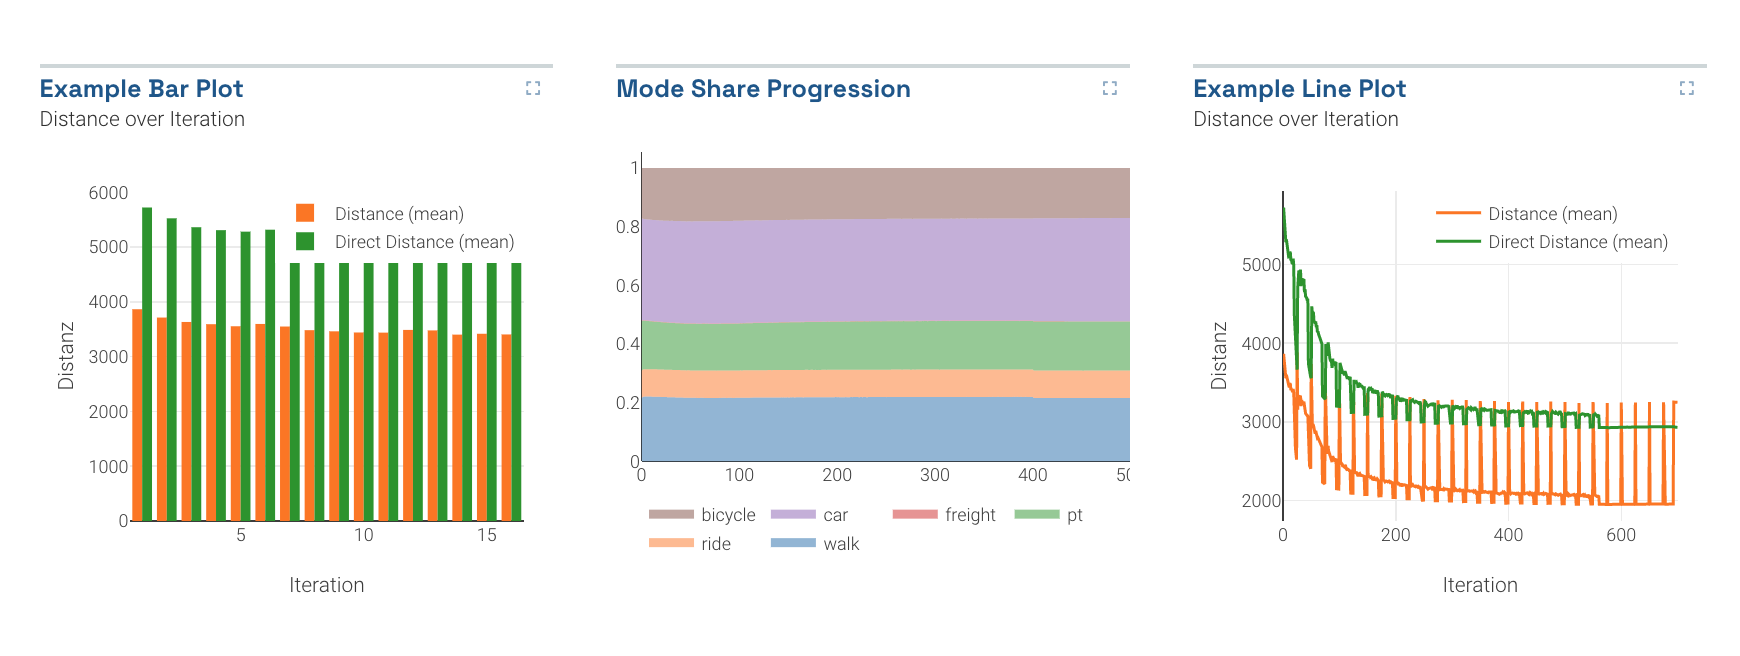
\includegraphics[width=0.8\textwidth]{assets/bar-line.png}
  \caption{Typical bar, area, and line charts}
\end{figure}

These simple charts comprise the core of many dashboards.

\hypertarget{usage}{%
\subsection{Usage}}

Bar, area, and line charts can only be included as panels in
\textbf{Dashboards}. See Dashboard documentation for general tips on
creating dashboard configurations.

\begin{itemize}
\tightlist
\item
  Each chart panel is defined inside a \textbf{row} in a
  \texttt{dashboard-*.yaml} file.
\item
  Choose from panel types \texttt{bar} \texttt{line} and \texttt{area}
  in the dashboard configuration.
\item
  Standard title, description, and width fields define the frame.
\end{itemize}

\begin{center}\rule{0.5\linewidth}{0.5pt}\end{center}

\hypertarget{sample-dashboard.yaml-config-snippet}{%
\subsubsection{Sample dashboard.yaml config
snippet}\label{sample-dashboard.yaml-config-snippet}}

\begin{lstlisting}
  layout:
  row1:
    - type: 'bar'
      title: 'Bar Plot'
      description: 'By iteration'
      width: 2
      dataset: '*drt_customer_stats.csv'
      x: 'iteration'
      xAxisName: 'Iteration'
      yAxisName: 'Distance'

    - type: 'area'
      title: 'Mode Share Progression'
      description: 'By iteration'
      width: 1
      dataset: '*modestats.txt'
      x: 'Iteration'

    - type: 'line'
      title: 'Mean Distances by Mode'
      description: 'per Iteration'
      width: 1
      dataset: '*drt_customer_stats.csv'
      x: 'iteration'
      xAxisName: 'Iteration'
      yAxisName: 'Distance'
      columns: [distance_m_mean, directDistance_m_mean]
      legendTitles: ['Distance (mean)', 'Direct Distance (mean)']

\end{lstlisting}

\hypertarget{bar-area-line-chart-properties}{%
\subsubsection{Bar, area, line chart properties}\label{bar-area-line-chart-properties}}

Each chart can have the following properties:

\noindent\textbf{dataset:} (Required) String. The filepath containing the data.
May include wildcards * and ?.

\noindent\textbf{x:} (Required) String. The column containing x-values.

\noindent\textbf{columns:} (Required) Array of strings. List the column names of
the columns which have the values to be graphed. Each element will be
its own line/color. Example:
\texttt{{[}\textquotesingle{}distance\textquotesingle{},\ \textquotesingle{}duration\textquotesingle{}{]}}

\noindent\textbf{useLastRow:} true/false. If set to true, only the last row of
the datafile will be used to build the pie chart. For example, this is
useful for MATSim outputs which list every iteration's output, and you
are only interested in the final iteration.

\noindent\textbf{stacked:} true/false for bar charts: whether to stack multiple
bars

\noindent\textbf{legendTitles:} Array of strings. Legend titles for each data
column. The column names will be used if this is omitted.

\noindent\textbf{xAxisName/yAxisName:} Labels for the axes.


\begin{center}\rule{0.5\linewidth}{0.5pt}\end{center}
\section{Reference: Sankey/Alluvial Diagrams}
\begin{figure}[H]
  \centering
  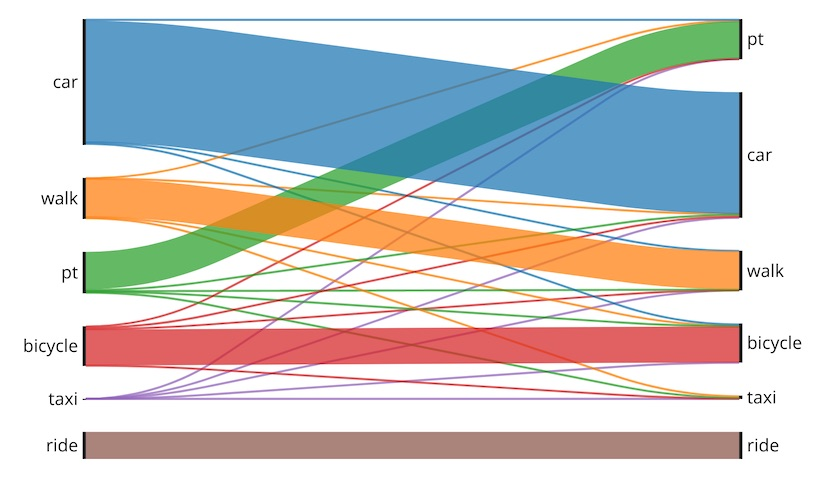
\includegraphics[width=0.8\textwidth]{assets/sankey.jpg}
  \caption{Mode shifts depicted as a Sankey diagram}
\end{figure}

Sankey diagrams are great for showing the shift between two states; for example
mode share shift from alt. A to alt. B. You see these a lot in politics
after a parliamentary election, to show the change in the number of
seats for each party.

\hypertarget{usage}{%
\subsection{Usage}}

Standalone: a file named \texttt{sankey-*.yml} must be present in
working folder. Each yml file matching that pattern will produce a
separate Sankey diagram.

Dashboard: Each panel is defined inside a \textbf{row} in a
\texttt{dashboard-*.yaml} file.

\begin{itemize}
\tightlist
\item
  Use panel \texttt{type:\ sankey} in the dashboard configuration.
\end{itemize}

\textbf{sankey-example.yml}

\begin{lstlisting}
  # only the csv line is required, but title and description help your viewers
  type: sankey
  csv: modeshares.csv
  title: Sankey Demo
  description: Erster Schritt!
\end{lstlisting}

\hypertarget{sankey-csv-file-format}{%
\subsection{Sankey CSV File format}\label{sankey-csv-file-format}}

Header line can contain labels but is CURRENTLY IGNORED

\begin{itemize}
\tightlist
\item
  Column 1: `From' category
\item
  Column 2: `To' category. These are not required to match the labels in
  column 1.
\item
  Column 3: Value
\item
  All other columns ignored
\end{itemize}

\textbf{Example:}

\begin{lstlisting}
from;to;number of trips (sample size); average change [sec]

car;car;748552;4.851276865
walk;walk;236111;0.064274854
walk;car;1644;-797.9385645
pt;ride;0;0
pt;bicycle;3167;-394.8995895
bicycle;walk;2276;925.78471

ride;bicycle;0;0
\end{lstlisting}


\begin{center}\rule{0.5\linewidth}{0.5pt}\end{center}
\section{Reference: Shapefiles, Area Maps, and GeoJSON}
\begin{figure}[H]
  \centering
  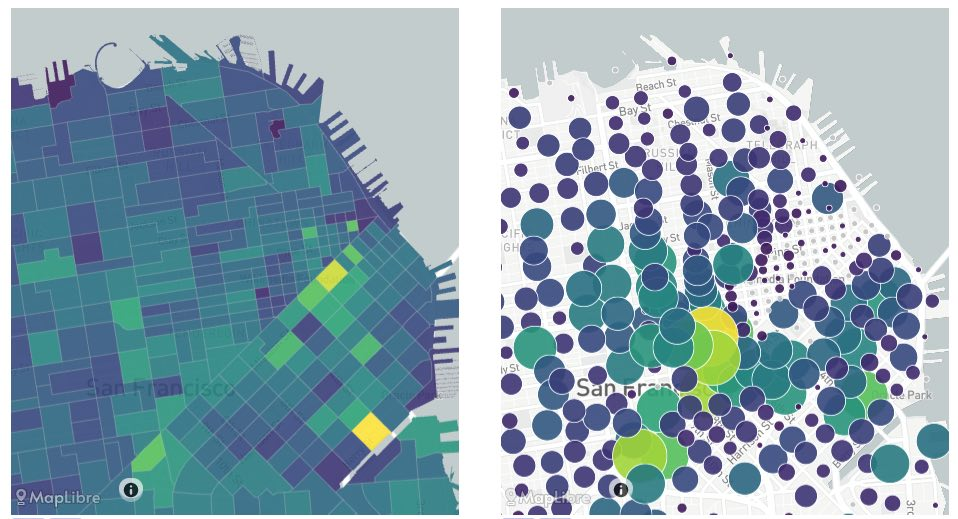
\includegraphics[width=0.8\textwidth]{assets/area-maps.jpg}
  \caption{Area map with color-filled areas; Area map with circles instead of filled areas}
\end{figure}

Area maps with filled colors are excellent for depicting spatial data in
one dimension.

\hypertarget{creating-this-panel}{%
\subsection{Creating this panel}\label{creating-this-panel}}

Properties are written in either a standalone \texttt{viz-map*.yaml}
file, or in a dashboard file they go in the \texttt{layout:} section of
a \texttt{dashboard-*.yaml} file. See the examples at the end of this
document.

\textbf{Standalone:} Create a \texttt{viz-map*.yaml} file as described
below

-or-

\textbf{Embed in Dashboard:} Create a \texttt{dashboard-*.yaml} file and
include a \texttt{type:\ map} section as described below.

\begin{itemize}
\tightlist
\item
  Each area map panel is defined inside a \textbf{row} in a
  \texttt{dashboard-*.yaml} file.
\item
  Use panel \texttt{type:\ map} in the dashboard configuration. (Note
  this may change in the future as we add more map types)
\item
  Standard title, description, and width fields define the frame.
\item
  See \href{dashboards}{Dashboard documentation} for general tips on
  creating dashboard configurations.
\end{itemize}

\hypertarget{properties}{%
\subsection{Properties}\label{properties}}

\hypertarget{dashboard-specific-properties}{%
\subsubsection{Dashboard-specific
properties}\label{dashboard-specific-properties}}

\begin{longtable}[]{@{}
  >{\raggedright\arraybackslash}p{(\columnwidth - 2\tabcolsep) * \real{0.5000}}
  >{\raggedright\arraybackslash}p{(\columnwidth - 2\tabcolsep) * \real{0.5000}}@{}}
\toprule()
\begin{minipage}[b]{\linewidth}\raggedright
Property
\end{minipage} & \begin{minipage}[b]{\linewidth}\raggedright
Usage
\end{minipage} \\
\midrule()
\endhead
\texttt{type} & In \texttt{dashboard-*.yaml} config files, MUST be set
to \textbf{``map''} \\
\texttt{height} & Relative height. Larger numbers create taller panels.
(default: 5) \\
\texttt{width} & Relative width. The widths of all panels on a single
row are summed, and the layout of each panel is then relative to that
total width. (default: 1) \\
\bottomrule()
\end{longtable}

\hypertarget{general-properties}{%
\subsubsection{General properties}\label{general-properties}}

\begin{longtable}[]{@{}
  >{\raggedright\arraybackslash}p{(\columnwidth - 2\tabcolsep) * \real{0.5000}}
  >{\raggedright\arraybackslash}p{(\columnwidth - 2\tabcolsep) * \real{0.5000}}@{}}
\toprule()
\begin{minipage}[b]{\linewidth}\raggedright
Property
\end{minipage} & \begin{minipage}[b]{\linewidth}\raggedright
Usage
\end{minipage} \\
\midrule()
\endhead
\texttt{title}, \texttt{title\_en}, \texttt{title\_de} & Title text for
this panel; will be shown just above the map. The language-specific
version will be used if provided. \\
\texttt{description}, \texttt{description\_en}, \texttt{description\_de}
& Second line of descriptive text, shown below the title line. The
language-specific version will be used if provided. \\
\texttt{center} & Coordinates that the map centers on. Can be provided
as array or string. If it is not provided, a center is calculated using
a sampling of the data. \\
\texttt{zoom} & Zoom level of the map between 5 and 20. (default: 9) \\
\texttt{pitch} & Map pitch (default: 0) \\
\texttt{bearing} & Map bearing/direction (default:0) \\
\bottomrule()
\end{longtable}

\hypertarget{shapes-the-boundariesareas-to-be-drawn}{%
\subsubsection{\texorpdfstring{\textbf{shapes:} the boundaries/areas to
be
drawn}{shapes: the boundaries/areas to be drawn}}\label{shapes-the-boundariesareas-to-be-drawn}}

There are \textbf{two separate data types} required for an area map: the
boundaries/shapes, and one the dataset (unless the shapefile
self-contains all of the required data).

Both files must contain an matching identification column in order to
\textbf{join the two datasets} together. In other words, the boundary
IDs must be present (somewhere) in both datafiles. The names of the
columns do not have to be identical, but it helps legibility. See below.

\begin{lstlisting}
shapes:
  file: my-taz-shapefile.shp
  join: id
\end{lstlisting}

Contains two subentries:

\begin{itemize}
\tightlist
\item
  \textbf{file:} String. The filepath containing the data. May include
  wildcards * and ?. File can be in \emph{geojson} format, or a
  \emph{shapefile}. File type is determined by suffix, so must end in
  either \texttt{.geojson} or \texttt{.shp} When loading shapefiles, an
  identically-named .dbf and .prj file will also be read from the same
  folder. Be sure to supply a .prj file containing a valid EPSG code if
  your data is not in lat/long format.
\item
  \textbf{join:} String. The name of the data column containing shape
  IDs, or `id' if it is in the id field of geojson.
\end{itemize}

\hypertarget{datasets-the-dataset-to-be-joined-to-the-shapefile}{%
\subsubsection{\texorpdfstring{\textbf{datasets:} the dataset to be
joined to the
shapefile}{datasets: the dataset to be joined to the shapefile}}\label{datasets-the-dataset-to-be-joined-to-the-shapefile}}

\begin{lstlisting}
  datasets:
    transit-trips:
      file: .summaries/transit-outputs.csv
      join: TAZ
\end{lstlisting}

Contains an object naming the dataset and providing its filename and
join column:

\begin{itemize}
\tightlist
\item
  \textbf{name of dataset:} Give the dataset a simple name, which will
  be used in the display settings below. e.g.~\texttt{tazdata}

  \begin{itemize}
  \tightlist
  \item
    \textbf{file:} String. The filepath containing the data. May include
    wildcards * and ?. File can be in \emph{CSV or DBF} format. Any
    filename not ending in \texttt{.dbf} will be parsed as a CSV file,
    using either commas, tabs, or spaces as delimiters.
  \item
    \textbf{join:} String. The name of the data column containing the
    shape IDs for joining.
  \end{itemize}
\end{itemize}

\hypertarget{display-define-the-color-and-value-details}{%
\subsubsection{\texorpdfstring{\textbf{display:} define the color and
value
details}{display: define the color and value details}}\label{display-define-the-color-and-value-details}}

For area maps, the \texttt{fill} section defines the color fill, and is
(currently) the only section that is required. At a later date we may
include borders, etc.

\begin{lstlisting}
display:
  fill:
    dataset: transit-trips
    join: TAZ
    filters: operator, income
    columnName: trip_origins, trip_boards, trip_reslocs
    colorRamp:
      ramp: Plasma
      reversed: true
      steps: 5
\end{lstlisting}

\textbf{dataset:} Name of the dataset from above which includes the
data.

\textbf{filters:} (optional) List of any columns which can be used as
category filters by the user interactively. Note that \emph{active
filters} will be shown in the URL bar, so curated maps can be shared via
URL.

\textbf{columnName:} The column name (or names) containing values to be
plotted. If multiple rows have a matching shape ID, all values will be
summed together. (Other stats to be added)

\textbf{colorRamp:} Describe the colors themselves:

\begin{itemize}
\tightlist
\item
  \textbf{ramp:} Name of the color ramp to use.

  \begin{itemize}
  \tightlist
  \item
    Sequential: \texttt{Viridis} \texttt{Plasma} \texttt{Blues}
    \texttt{Greens} \texttt{Purples} \texttt{Oranges}
  \item
    Diverging: \texttt{PRGn} \texttt{RdBu}
  \item
    Categorical: \texttt{Tableau10} \texttt{Paired}. Note categoricals
    only have ten or twelve categories.
  \end{itemize}
\item
  \textbf{reversed:} true/false
\item
  \textbf{steps:} Number of steps in the ramp.
\item
  \textbf{exponentColors:} Optional true/false. If true, values will be
  scaled exponentially before being drawn. This is often useful if
  values are concentrated in small areas, and much higher in value than
  in typical areas.
\item
  \textbf{diff:} Example \texttt{col1\ -\ col2} will activate diff mode

  \begin{itemize}
  \tightlist
  \item
    \emph{(todo: more examples needed )}
  \end{itemize}
\end{itemize}

\hypertarget{filters}{%
\subsubsection{filters}\label{filters}}

In the \texttt{filter} section, you can filter dataset with multiple
expressions on numerical columns in any dataset. Keys are of the format
\texttt{dataset.column:\ "filter"} and filter can be
\texttt{==,\ !=,\ \textless{},\ \textless{}=,\ \textgreater{},\ \textgreater{}=}

\begin{lstlisting}
filters:
  dataset1.trips: "> 0"
  shapes.TAZ: "!=0"

\end{lstlisting}

\hypertarget{tooltip}{%
\subsubsection{Tooltip}\label{tooltip}}

By default, the tooltip shows all columns in the shapefile, as well as
any columns that are actively being displayed as either a color or a
width.

You can customize the tooltip to just show what you are interested as
follows:

\begin{itemize}
\tightlist
\item
  Add a \texttt{tooltip:} section to the properties, which will be an
  array of tooltip entries
\item
  Each entry is of format \texttt{datasetname:columnname}, so for
  example \texttt{AM\_FLOWS:VEHICLE\_VOL} will display the AM\_FLOWS
  dataset and VEHICLE\_VOL column.
\item
  Use the shapefile/network filename for its columnar data, or the
  dataset ``key'' for joined datasets.
\end{itemize}

\textbf{Custom tooltip example:}

\begin{lstlisting}
tooltip:
  - AM:TOT_VOL
  - AM:TNC
  - freeflow.shp:FACILITY_TYPE
  - freeflow.shp:SPEED
\end{lstlisting}

\hypertarget{visualization-hints}{%
\subsection{Visualization hints}\label{visualization-hints}}

Very large and very small areas on the same maps can create misleading
visualizations; consider ``normalizing'' data by land area before
plotting it. Alternatively, the circle-plots show exactly the same data
in a different manner.

\begin{itemize}
\tightlist
\item
  Use the sequential color palettes for continuous data.
\item
  Use diverging color palettes for difference plots and other situations
  where data is both positive and negative
\item
  Use categorical colors when there are just a few categories or
  ``buckets'' in which the data resides.
\end{itemize}

\hypertarget{example-yaml-configurations-putting-it-all-together}{%
\subsection{Example YAML configurations: putting it all
together}\label{example-yaml-configurations-putting-it-all-together}}

\hypertarget{sample-viz-map-1.yaml-standalone-configuration}{%
\subsubsection{Sample viz-map-1.yaml standalone
configuration}\label{sample-viz-map-1.yaml-standalone-configuration}}

\begin{lstlisting}
  title: 'VIZ-MAP 1'
  description: 'All day transit usage'
  center: [6.9814, 51.57]
  zoom: 10
  shapes:
    file: '../../shapefiles/geoid.geojson'
    join: id
  datasets:
    transit-trips:
      file: .dashboard/transit-data.csv
  display:
    fill:
      dataset: transit-trips
      join: geoid
      filters: operator, income
      columnName: trip_origins, trip_boards, trip_reslocs
      colorRamp:
        ramp: Plasma
        steps: 7
\end{lstlisting}



\begin{center}\rule{0.5\linewidth}{0.5pt}\end{center}
\section{Reference: XY Hexagon Aggregated Point Data}
\begin{figure}[H]
    \centering
    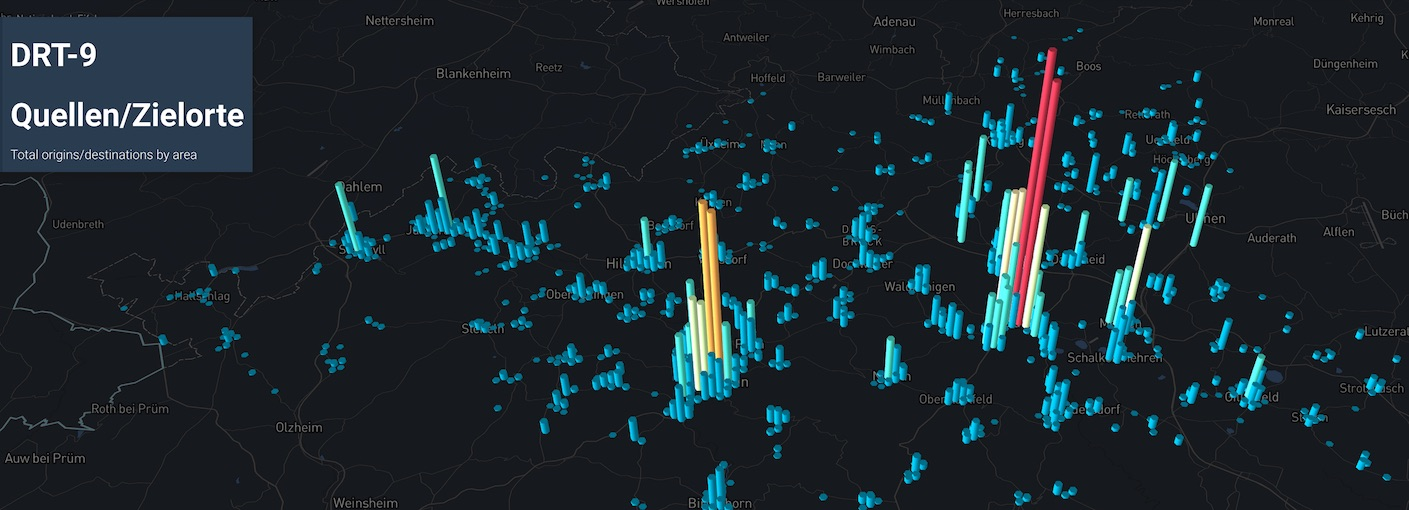
\includegraphics[width=0.8\textwidth]{assets/xy-hexagons.jpg}
    \caption{Origin/Destination point data aggregated into hexagons}
\end{figure}

Counts the number of points that occur inside hexagons of arbitrary size.

\hypertarget{usage}{%
\subsection{Usage}}

A file named \texttt{viz-xy-*.yml} will match and trigger the creation
of the XY hexagon plot.

In addition, the presence of the MATSim regular output file
\texttt{output-trips.xml.gz} will automatically trigger an XY Hexagon
plot depicting the trip origins and destinations present in that file.

\hypertarget{dashboards}{%
\subsection{Dashboards}}

XY Hexagon plots can be embedded in dashboards using
\texttt{type:\ hexagons} and specifying the config details in the props
as follows:

\begin{lstlisting}
row:
- title: My Hexagon Plot
    type: hexagons
    # ...
\end{lstlisting}

\hypertarget{yaml-fields-explained}{%
\subsection{YAML fields explained}}

These YAML fields are supported:

\textbf{title:} (optional) title of the visualization, appears right on
top of the map. If a title is specified both under ´general´ and under
´props´, the one under ´general´ will be used.

\textbf{description:} (optional) description of the visualization,
appears between title and map. If a description is specified both under
´general´ and under ´props´, the one under ´general´ will be used.

\textbf{file:} a csv, json or gzip'ed json file containing an array with
the data.

\textbf{projection:} EPSG code of the projection

\textbf{elements:} the name of the property containing the data array
(for JSON files only)

\textbf{thumbnail:} (optional) file path to a thumbnail in jpg format

\textbf{center:} (optional) coordinates that the map centers on. Can be
provided as array or string. If it is not provided, a center is
calculated using a sampling of the data.

\textbf{zoom:} (optional) zoom level of the map between 5 and 20. If it
is not provided, the zoom level 9 is used.

\textbf{radius:} starting radius of the hexagons.

\textbf{maxHeight:} (optional) starting height of the hexagons. If it is
not provided, 0 is used.

\textbf{aggregations:} a list of \texttt{title}, \texttt{x}, \texttt{y}
which say which columns of data in the elements array contain the x,y
data. x,y can be column numbers or column names. You can specify
multiple aggregations in the data section. \emph{Note: column numbers
are zero-based!}

\hypertarget{xy-data-file-format}{%
\subsection{XY Data File format}\label{xy-data-file-format}}

JSON and CSV files are supported.

\textbf{CSV:} a simple CSV with a header column is all that's needed.

\textbf{JSON}: The file must have an object with a property whose name
is the element. Here's an example that matches the sample YML above.

In this example, each array element is also an array with xy data in
columns 0,1 and 3,4. The row elements can also be regular JSON objects,
in which case the x/y columns can be referenced by name instead number.

\begin{lstlisting}
{
    "drtRequests": [
        [ 6.2343, 52.123, 0, 6.33, 52.23, 0],
        [ 7.0341, 51.237, 0, 7.81, 51.44, 0],
        ...
    ]
}
\end{lstlisting}

All other elements in the JSON are ignored.

\hypertarget{example-yaml-configs}{%
\subsection{Example YAML configs}\label{example-yaml-configs}}

\textbf{viz-xy-example.yml}

\begin{lstlisting}
title: 'XY Example-1: DRT Vehicles'
description: 'Total origins/destinations by area'
file: drt-vehicles.json.gz
thumbnail: thumbnail-vehicles.jpg
center: [6.9814, 51.57]
zoom: 10
radius: 200
maxHeight: 30
elements: drtRequests # only if json
aggregations:
    OD Summary:
    - title: Origins
        x: fromX
        y: fromY
    - title: Destinations
        x: toX
        y: toY
    Base Runs:
    - title: Origins
        x: baseFromX
        y: baseFromY
    - title: Destinations
        x: baseToX
        y: baseToY
\end{lstlisting}



\begin{center}\rule{0.5\linewidth}{0.5pt}\end{center}
\section{Reference: X/Y/Time Disaggregate Point Data}
\begin{figure}[H]
  \centering
  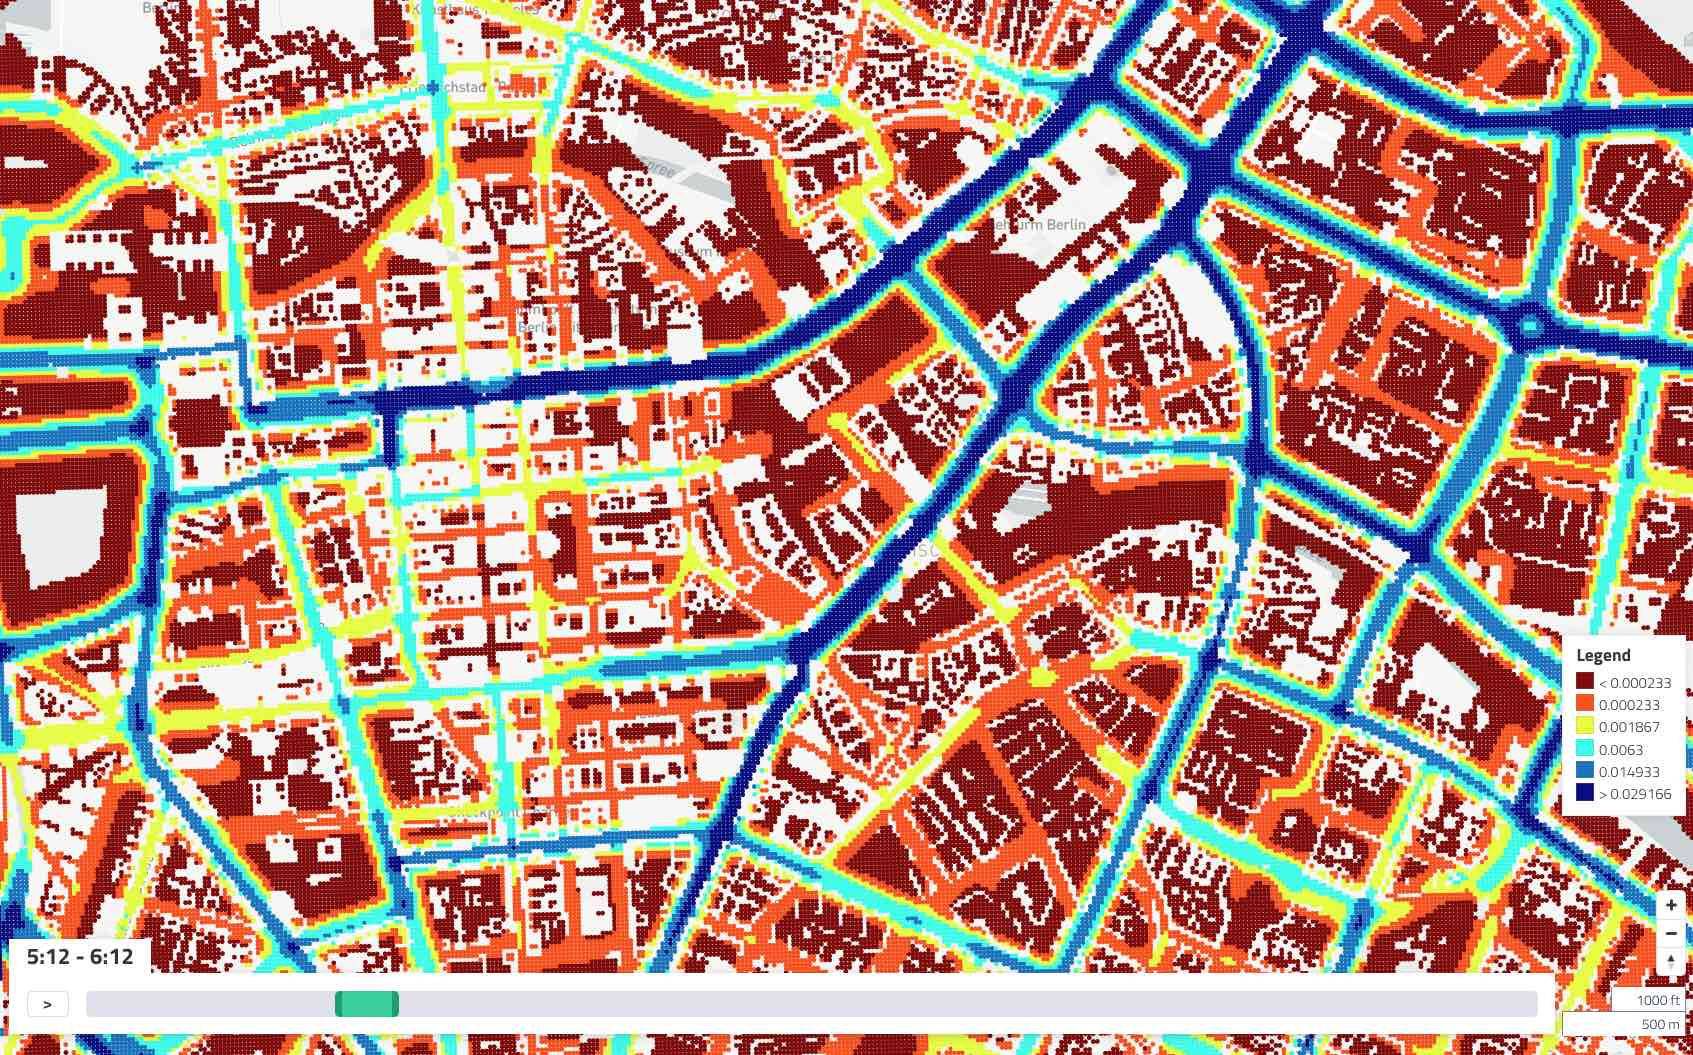
\includegraphics[width=0.8\textwidth]{assets/xyt-emissions.jpg}
  \caption{X/Y/Time point-based emissions data example}
\end{figure}

Display disaggregate point data with a time component; useful for
emissions, noise, etc.

We are currently researching the best way to ingest very large
X/Y/Time data files.

Currently, SimWrapper can load an \texttt{*.xyt.csv} file
but it takes a long time (up to a few minutes for some simulations), and
then the viz displays.

\hypertarget{usage}{%
\subsection{Usage}}

If a file with name matching \texttt{*.xyt.csv} exists in a folder, the
X/Y/T viewer will be available. There is no YAML configuration
available, but there is an interactive panel for modifying the color
attributes.



\end{appendices}
%\cleardoublepage

% =======================================================
%%%%%%%%%%%%%%%% Acronyms %%%%%%%%%%%%%%%
% =======================================================
\glsaddall
\printglossary[type=\acronymtype,title=List of Units and
Acronyms, toctitle=List of Units and Acronyms]
\cleardoublepage

% =======================================================
%%%%%%%%%%%%%% Literaturverzeichnis %%%%%%%%%%%%%
% =======================================================
\phantomsection
\raggedright
\renewcommand\bibfont{\small}
\renewcommand{\UrlFont}{\ttfamily\scriptsize}
%\renewcommand*\backref[1]{\ifx#1\relax \else (cited on p. #1) \fi}
\renewcommand*{\backreflastsep}{, }
\renewcommand*{\backreftwosep}{, }
\renewcommand*{\backref}[1]{}
\renewcommand*{\backrefalt}[4]{%
   \ifcase #1 %
     No citations.% use \relax if you do not want the "No citations" message
   \or
     (cited on p. #2).%
   \else
     (cited on pp. #2).%
   \fi%
}
\setstretch{1}
\bibliography{book,ref,vsp,thesis}
\bibliographystyle{bib/bibstyle}
%\bibliographystyle{plain}
\cleardoublepage
\newpage
\thispagestyle{empty}
\mbox{}
%%%%%%%%%%%%%%%%%%%%%%%%%%%%%%%%%%%%%%
%\todo[inline]{Lösche Todo-Listen}
%\todo[inline]{makeglossary command ausführen}
%\todo[inline]{Enteferne allgmeine Notizen/Fragen Bereich aus dem Dokument}
%%%%%%%%%%%%%%%%%%%%%%%%%%%%%%%%%%%%%%
\end{document}
